\chapter{Network Layer:\\ A Custom Embedded-Oriented Protocol}\label{sec:protocol}

\section{Background}\label{sec:protocol:background}

A variety of protocols exist that are geared toward different types of networks. Section \ref{sec:protocol:background:switching} will consider a variety of switching techniques. Section \ref{sec:protocol:background:protocols} will consider two popular protocols currently in widespread use: the Internet Protocol Suite, also known as Transmission Control Protocol and Internet Protocol (TCP/IP) over Ethernet, and RapidIO. Switching is discussed first because the switching techniques employed in a given protocol generally influence the information that a protocol includes in its packet headers. Finally, communication faults are discussed in Section \ref{sec:protocol:introduction:communication_faults}.

\subsection{Overview of Select Existing Switching Mechanisms}\label{sec:protocol:background:switching}

Switching techniques determines how a data packet is forwarded through a network. Switching is not to be confused with routing, which determines \emph{where} a data packet is sent in the network. The switching technique determines if and how links are reserved, the relationship between the header and the data payload as they travel through the network, etc. Many different types of switching exist, so this section will focus on the following basic types of switching: virtual circuit switching, packet switching, virtual cut-through switching, wormhole switching, and pipelined circuit switching.
Circuit switching was originally developed for the Plain Old Telephone System (POTS) and is called circuit switching because the early automated switching devices used electro-mechanical circuits configured in an array to connect one end to the other. Circuit switching in modern information networks (called Virtual Circuit Switching) uses completely different hardware, of course, but many of the basic principles still apply. The main differentiating characteristic of circuit switching is that a network path is reserved \emph{prior} to sending any data. The path is typically reserved by first sending a ``probe'' packet. This packet is sent to the destination, and each node the probe passes through reserves the appropriate links. When the entire path is reserved, the destination sends an acknowledgement back to the sender indicating that data transmission can commence. The data packet is then transferred along the reserved path. The time-space diagram of a packet being sent through a virtual circuit switching network is shown in Figure \ref{fig:protocol:vcs_time_diagram}. In the figure, $t_r$ is the processing time spent making routing decisions and $t_s$ is the processing time spent making switching decisions. The primary advantages of circuit switching are that it is simple to implement and that it is very reliable after a path is established. The primary downside to circuit switching is that after a path is reserved, no other transfers can use those links, which can increase congestion. Circuit switching is advantageous in networks where packets are infrequent and long. \cite{ref:1997-duato-interconnection_networks}

\begin{figure}[ptb]
	\begin{centering}
		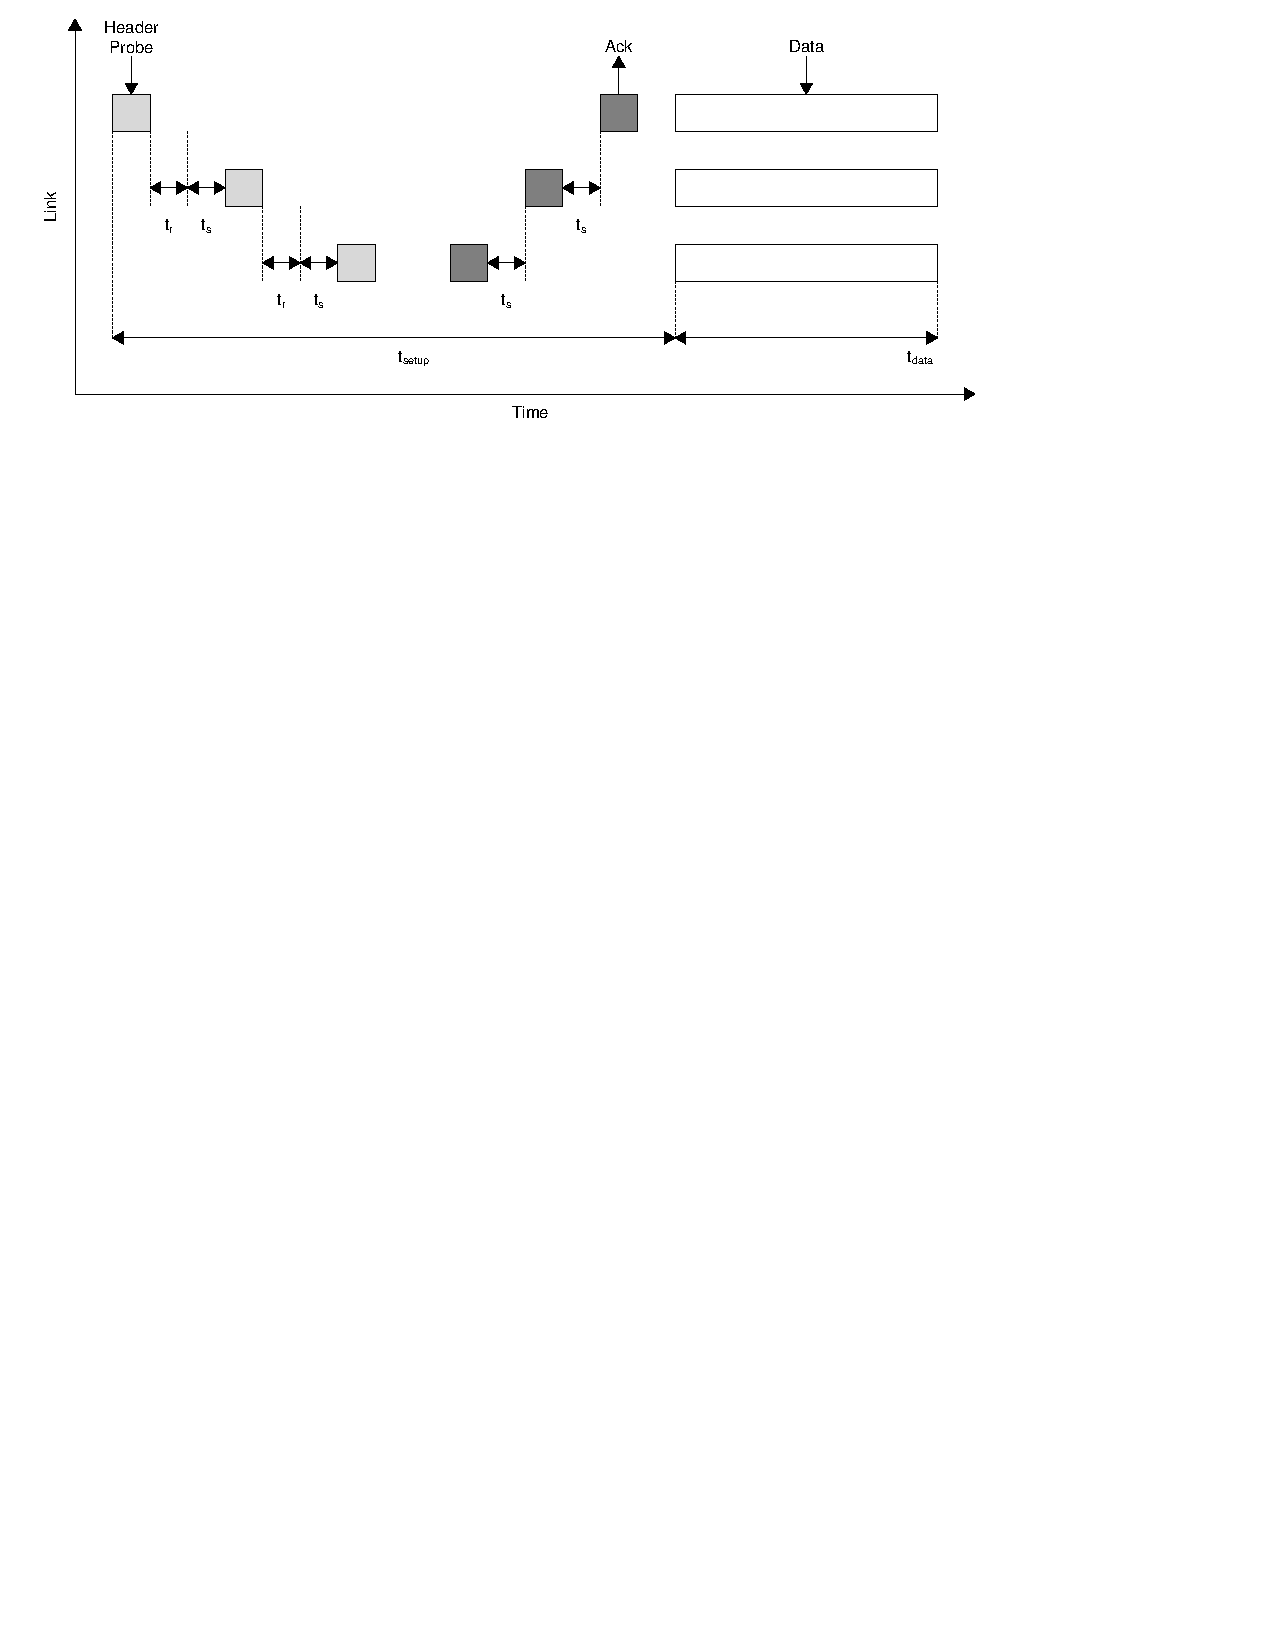
\includegraphics[scale=0.8]{Protocol/Figures/protocol-vcs_time_diagram.pdf}
		\caption[Virtual Circuit Switching Time Diagram]{Virtual Circuit Switching Time Diagram \cite{ref:1997-duato-interconnection_networks}}
		\label{fig:protocol:vcs_time_diagram}
	\end{centering}
\end{figure}

Packet switching does not reserve a channel prior to transmitting and instead transmits the data payload with the packet header. Packet switching works best with small packet sizes, so large messages are typically broken into multiple smaller packets. Each packet contains its own header and is routed independently of the other packets to the destination. Every packet is fully buffered at each node $x$, and then forwarded to the next node. This mechanism makes packet switching very robust to congestion, but at the expensive of more overhead in the packet headers and in processing at each node. In particular, packet switching requires large amounts of buffer storage at each node so it can potentially buffer several complete packets at a time, which is something that is often not possible in embedded processors. The time-space diagram is shown in Figure \ref{fig:protocol:ps_time_diagram}. Packet switching is advantageous in networks where packets are frequent and short. \cite{ref:1997-duato-interconnection_networks}

\begin{figure}[ptb]
	\begin{centering}
		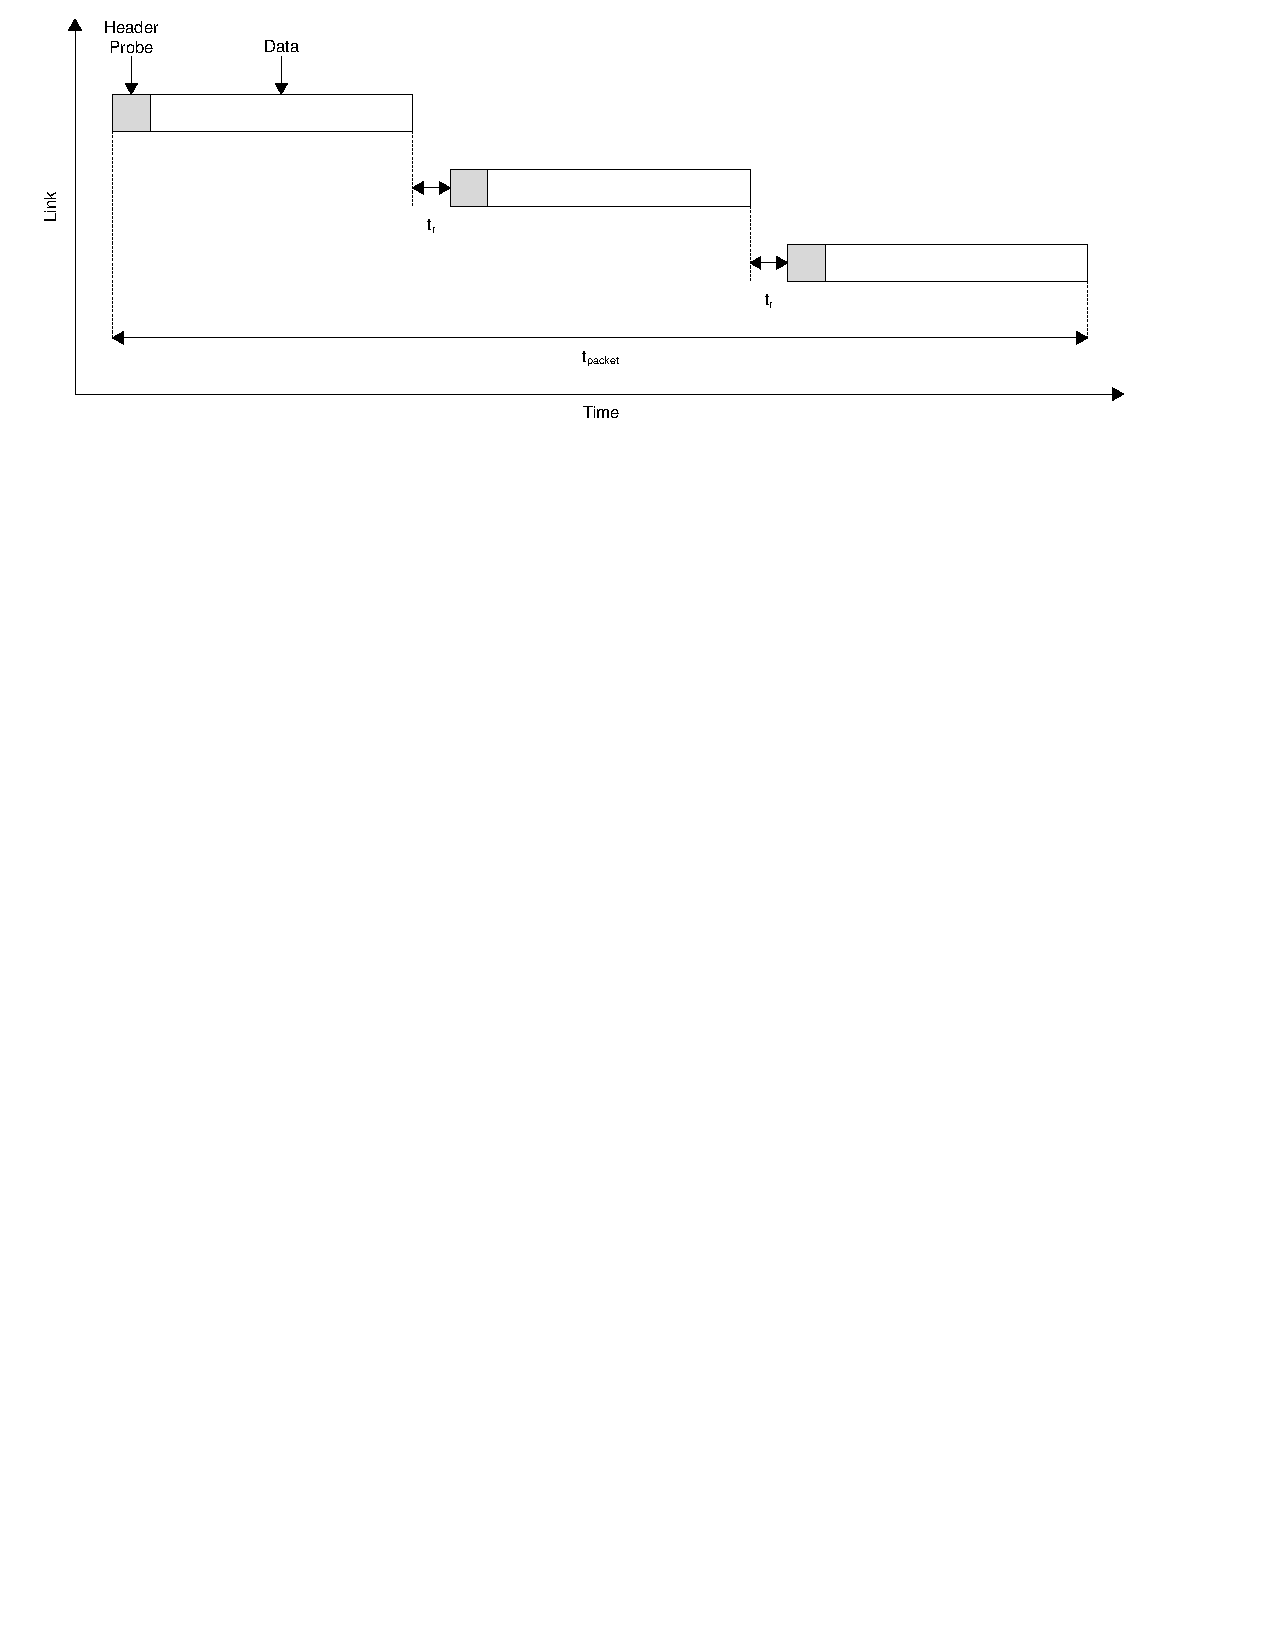
\includegraphics[scale=0.8]{Protocol/Figures/protocol-ps_time_diagram.pdf}
		\caption[Packet Switching Time Diagram]{Packet Switching Time Diagram \cite{ref:1997-duato-interconnection_networks}}
		\label{fig:protocol:ps_time_diagram}
	\end{centering}
\end{figure}

Virtual cut-through switching is a modified version of packet switching that takes advantage of the fact that packet headers occur at the beginning of a packet. This mechanism allows a node to inspect the header as soon as it has arrived and to determine what to do with the packet. The node then begins forwarding data as soon as it arrives. In the case of a blocked path, the entire message is buffered at the node. This eliminates the need for large data buffers in the network because flits can be forwarded as soon as they arrive, and it is reasonable to assume that there won't be a ``pile-up'' of blocked messages. The time-space diagram is shown in Figure \ref{fig:protocol:vcts_time_diagram}. Virtual cut-through switching does decrease latency and buffer capacity, but still suffers from high complexity. \cite{ref:1997-duato-interconnection_networks}

\begin{figure}[ptb]
	\begin{centering}
		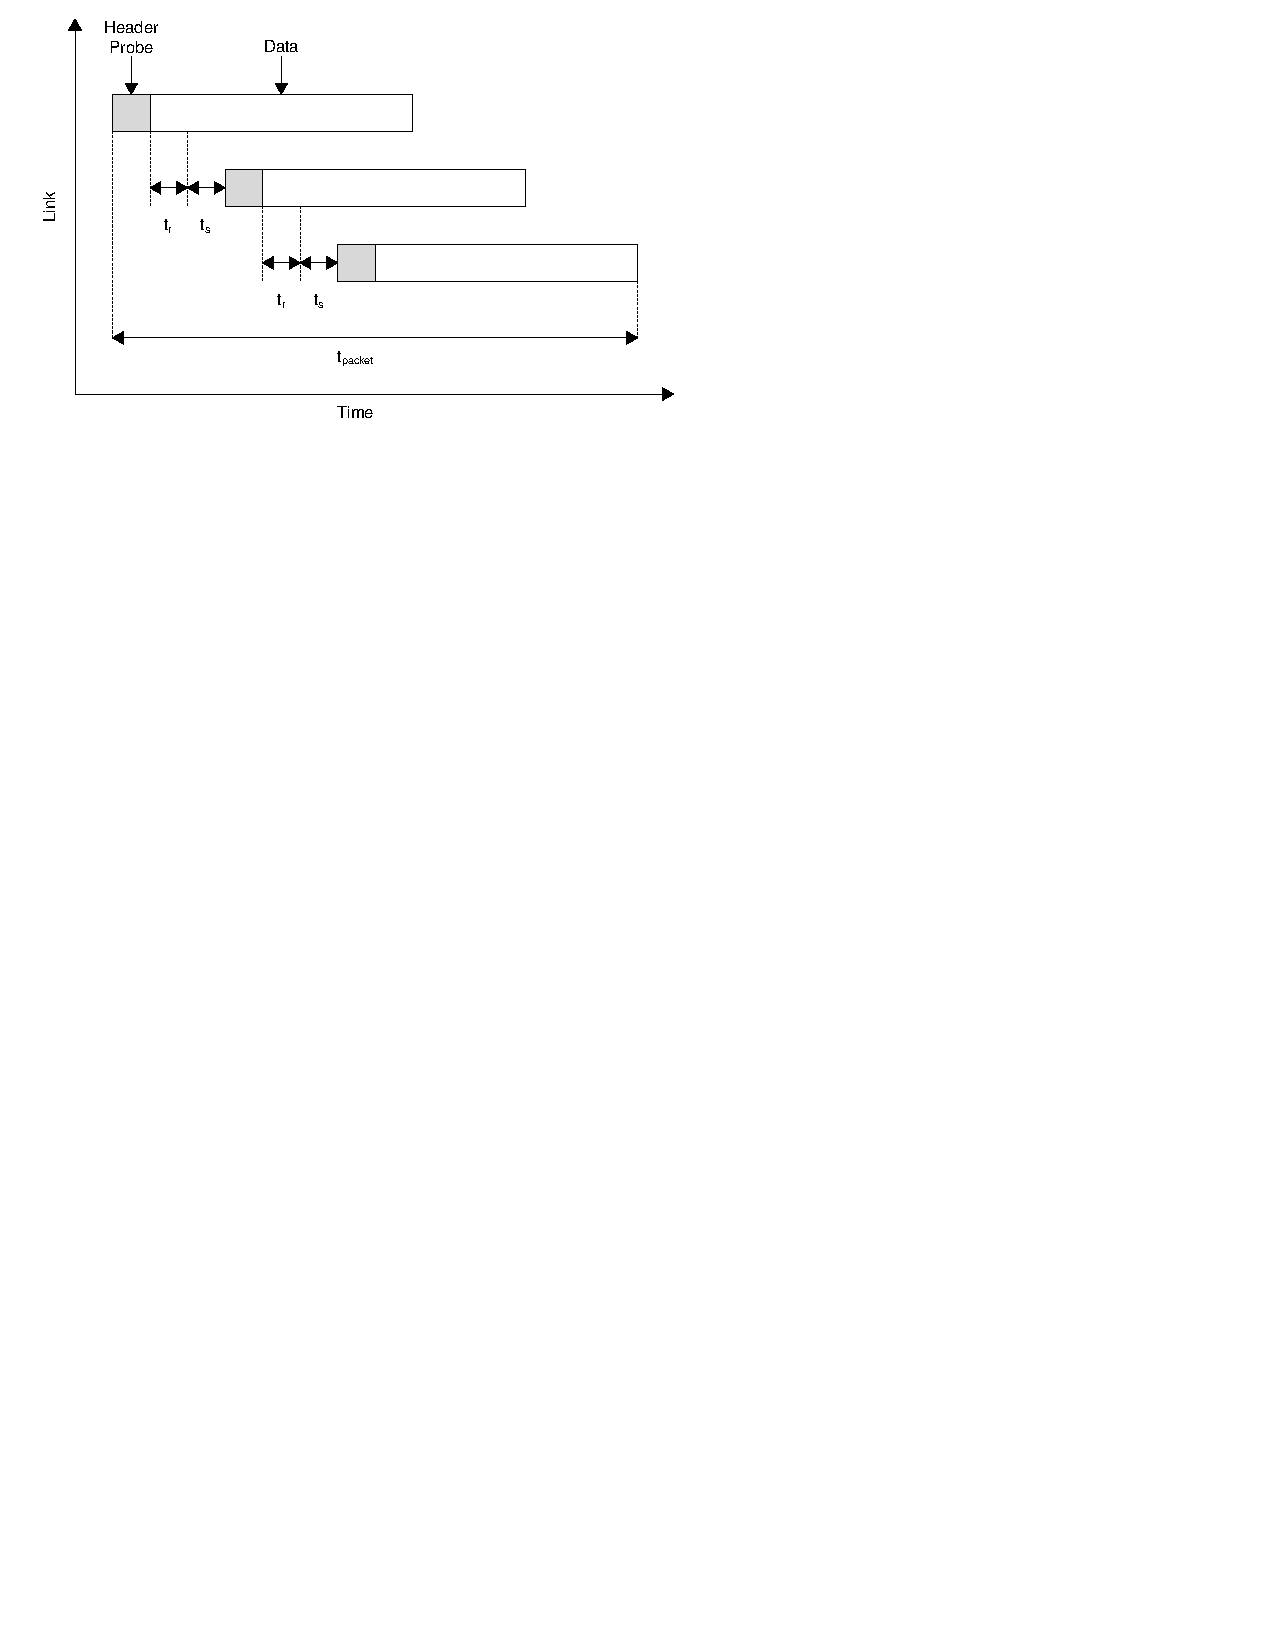
\includegraphics[scale=0.8]{Protocol/Figures/protocol-vcts_time_diagram.pdf}
		\caption[Virtual Cut-Through Switching Time Diagram]{Virtual Cut-Through Switching Time Diagram \cite{ref:1997-duato-interconnection_networks}}
		\label{fig:protocol:vcts_time_diagram}
	\end{centering}
\end{figure}

Wormhole switching is very similar to virtual cut-through switching in that it begins forwarding flits as soon as they are available. The key difference between virtual cut-through switching and wormhole switching is how they deal with blocked links. In wormhole switching, a blocked path results in the transmission ``stalling'' where it is. In other words, transmission stops where it is, leaving the packet spread across multiple routers. As a result, the complexity is higher than virtual cut-through switching, but it requires significantly smaller buffers compared to virtual cut-through switching. The time-space diagram for wormhole routing is shown in Figure \ref{fig:protocol:ws_time_diagram}. \cite{ref:1997-duato-interconnection_networks}

\begin{figure}[ptb]
	\begin{centering}
		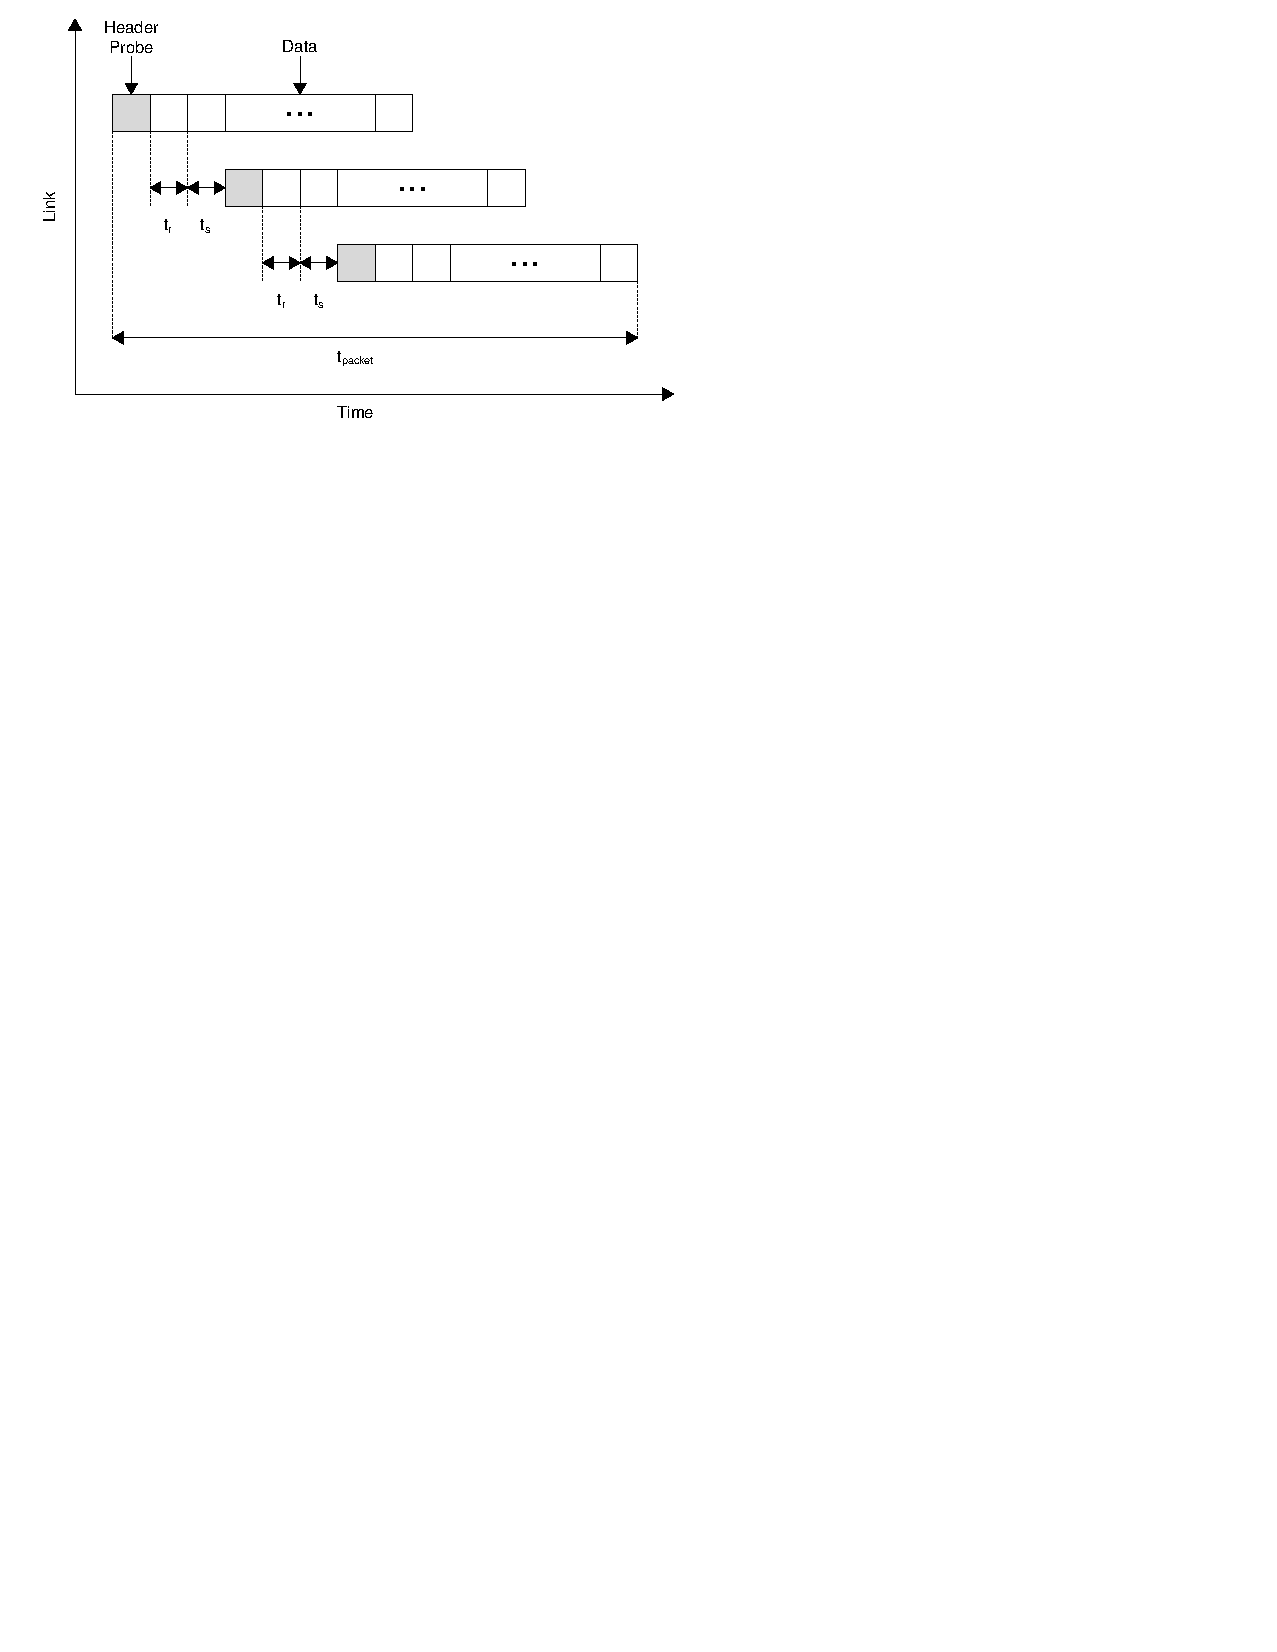
\includegraphics[scale=0.8]{Protocol/Figures/protocol-ws_time_diagram.pdf}
		\caption[Wormhole Switching Time Diagram]{Wormhole Switching Time Diagram \cite{ref:1997-duato-interconnection_networks}}
		\label{fig:protocol:ws_time_diagram}
	\end{centering}
\end{figure}

Pipelined circuit switching is designed to make wormhole routing more fault tolerant, at the expense of performance. In wormhole routing, if the header gets stuck somewhere due to a faulty component or blocked link, the data payload stalls in the network, leaving the resources unavailable for other transfers. In pipelined circuit switching, instead of sending the data payload immediately after sending the header, the connection is first reserved using the same mechanisms as virtual circuit switching and then the data payload is sent. In order to prevent blocked messages, virtual channels, described in Chapter \ref{sec:spi}, are utilized. This method is called a ``hybrid'' switching technique because it combines elements of wormhole routing and virtual circuit routing. Pipelined circuit switching requires very small buffers, as in wormhole routing, but it also has the fault tolerance of virtual circuit routing and is very good at avoiding blocked links, while also being considerably simpler. The time-space diagram for pipelined circuit switching is shown in Figure \ref{fig:protocol:pcs_time_diagram}. \cite{ref:1997-duato-interconnection_networks}

\begin{figure}[ptb]
	\begin{centering}
		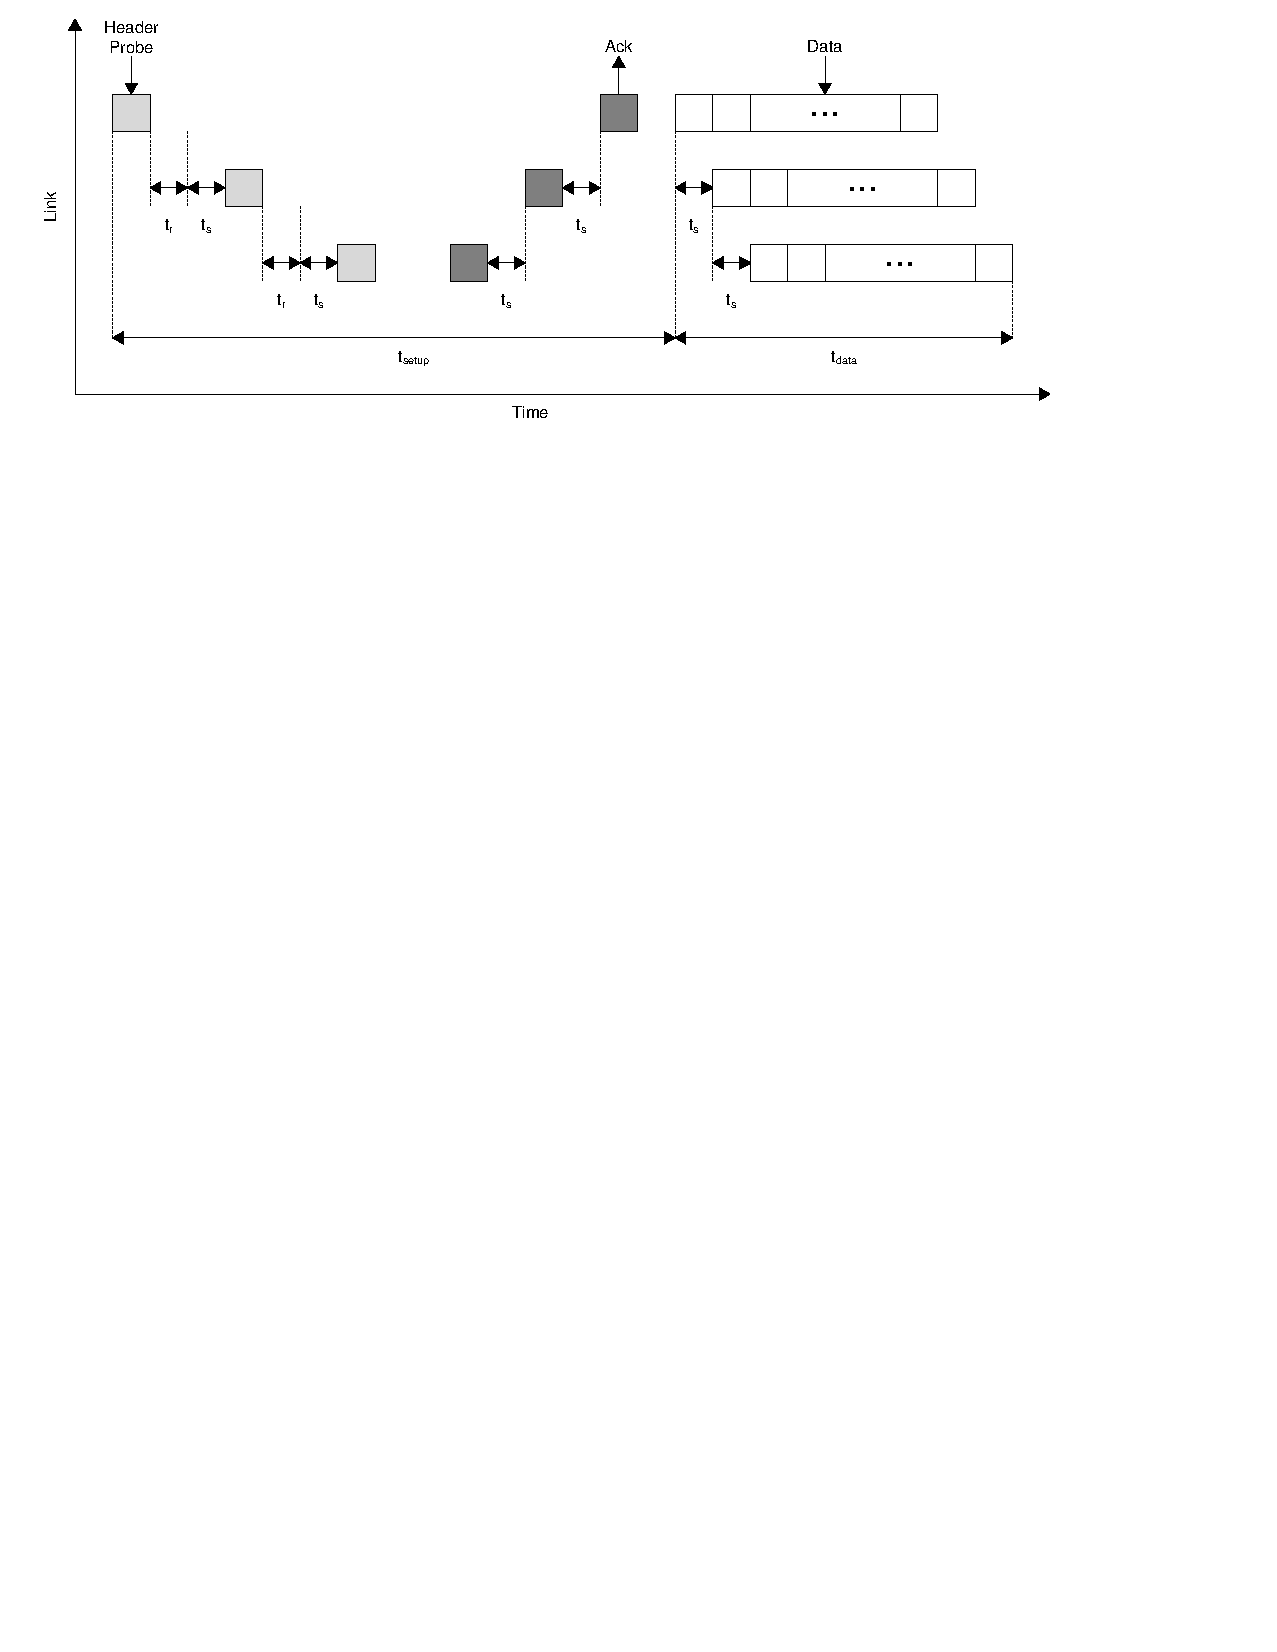
\includegraphics[scale=0.8]{Protocol/Figures/protocol-pcs_time_diagram.pdf}
		\caption[Pipelined Circuit Switching Time Diagram]{Pipelined Circuit Switching Time Diagram \cite{ref:1997-duato-interconnection_networks}}
		\label{fig:protocol:pcs_time_diagram}
	\end{centering}
\end{figure}

\subsection{Overview of Select Existing Protocols}\label{sec:protocol:background:protocols}

A variety of protocols exist that have been developed for different purposes. TCP/IP is ubiquitous in large scale networks and is the protocol used by personal computers and the Internet. Other protocols have been used in the past, such as NetBIOS over IPX/SPX, but have fallen out of favor in exchange for TCP/IP. Other protocols in use tend to be more special purposes than TCP/IP. PCI Express (PCIe), for example, is used to connect peripherals in a personal computer to the main processor. RapidIO has recently become popular in high-end embedded systems.

\subsubsection{TCP/IP Overview}\label{sec:protocol:background:protocols:tcpip}

TCP/IP is a suite of layered protocols that provide the primary protocols used for intranets and the Internet. The term TCP/IP is often used to denote different things depending on the context. For the purposes of this discussion, TCP/IP will refer to the protocols in the network and transport layers, but not in the data link/application/etc layers. TCP/IP is run on many different types of data link layers, but the most common is Ethernet. Ethernet is a shared medium physical and data link layer protocol and is analogous to the peer-to-peer mechanism described in Section \ref{sec:spi}.  Ethernet utilizes a 22 byte header, shown in Figure \ref{fig:protocol:ethernet_header}, which adds overhead to the system. The header is responsible for conditioning the signal, specifying source and destination hardware addresses, and specifying the data length. Ethernet switches typically use packet switching, although some variations exist. \cite{ref:2004-forouzan-data_communications_and_networking}

\begin{landscape}
	\begin{figure}[p]
		\begin{centering}
			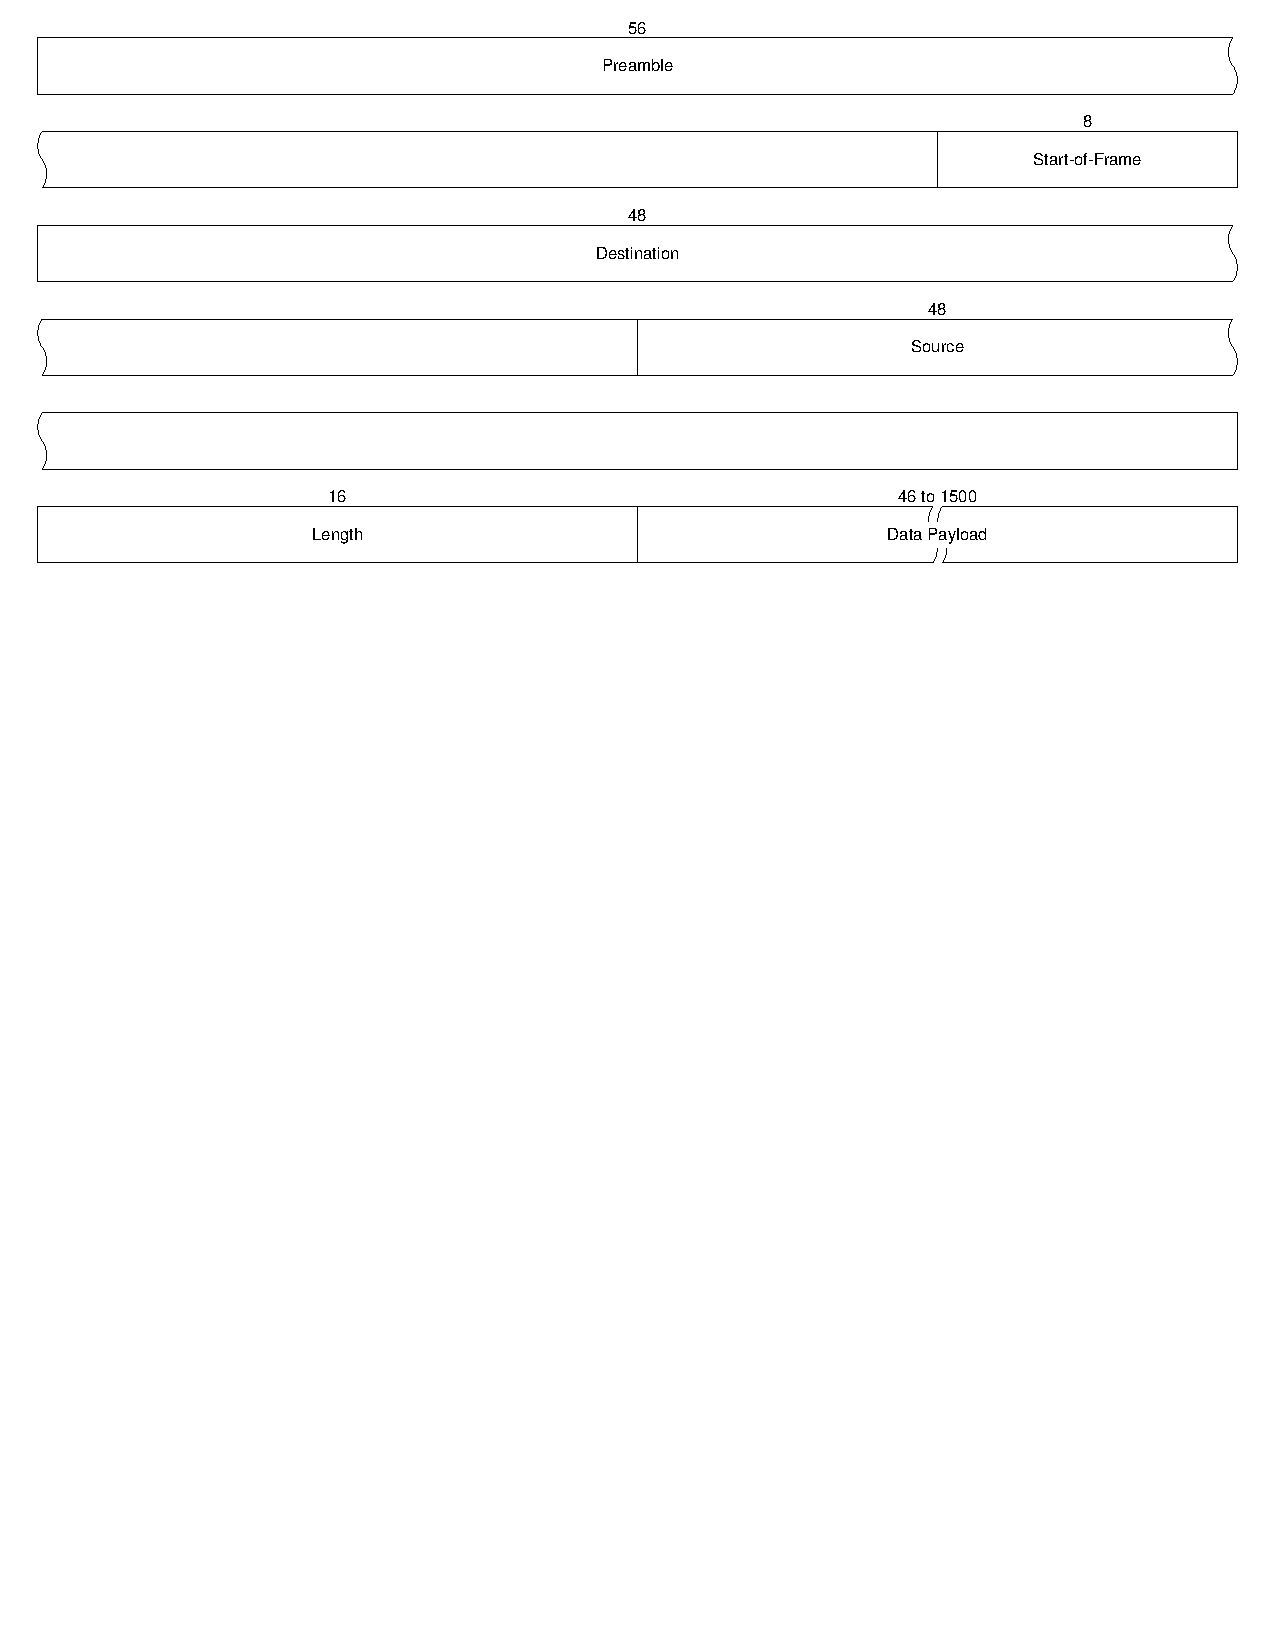
\includegraphics{Protocol/Figures/protocol-ethernet_header.pdf}
			\caption[Ethernet Header]{Ethernet Header \cite{ref:2004-forouzan-data_communications_and_networking}}
			\label{fig:protocol:ethernet_header}
		\end{centering}
	\end{figure}
\end{landscape}

The most important TCP/IP protocol at the network layer is the IP protocol. This protocol handles data transmissions originating from the higher layers. The other protocols are generally management-oriented or extend the IP protocol. The current IP protocol, IPv4, has been around for almost 30 years and will soon be replaced by IPv6. Due to the prevalence of IPv4, however, this paper will only consider it. IPv4 accepts data from the transport layer, packages it into an IP packet, and sends it to the data link layer. In the context of the Internet, IPv4 is responsible for delivering the packet to the final destination. By itself, IPv4 uses universal addresses for all nodes. These IP addresses are assigned by central authorities, such as the Internet Corporation for Assigned Names and Numbers (ICANN). Technologies such as Network Address Translation (NAT) allow private IP addresses that are not universally unique. IPv4 does not specify how to route a packet, and IPv4 supports arbitrary data fragmentation. These features allow IPv4 to be used on different types of networks with different types of routing protocols and packet lengths. The IPv4 header is shown in Figure \ref{fig:protocol:ip_header}. The options field in the header is the only variable length field, and usually isn't used. When unused, the total header length is 20 bytes long. The source and destination specify the initial source and final destination of the transfer, respectively. There is also a header checksum, assortment of flags, packet ID, and other information.  The fragment offset specifies where a data fragment fits into the full packet. Note that this implies, interestingly enough, that the process of partitioning the data into fragments and reassembling them on the other side \emph{is not handled} by IP. \cite{ref:2005-kozierok-tcpip_guide}

\begin{landscape}
	\begin{figure}[p]
		\begin{centering}
			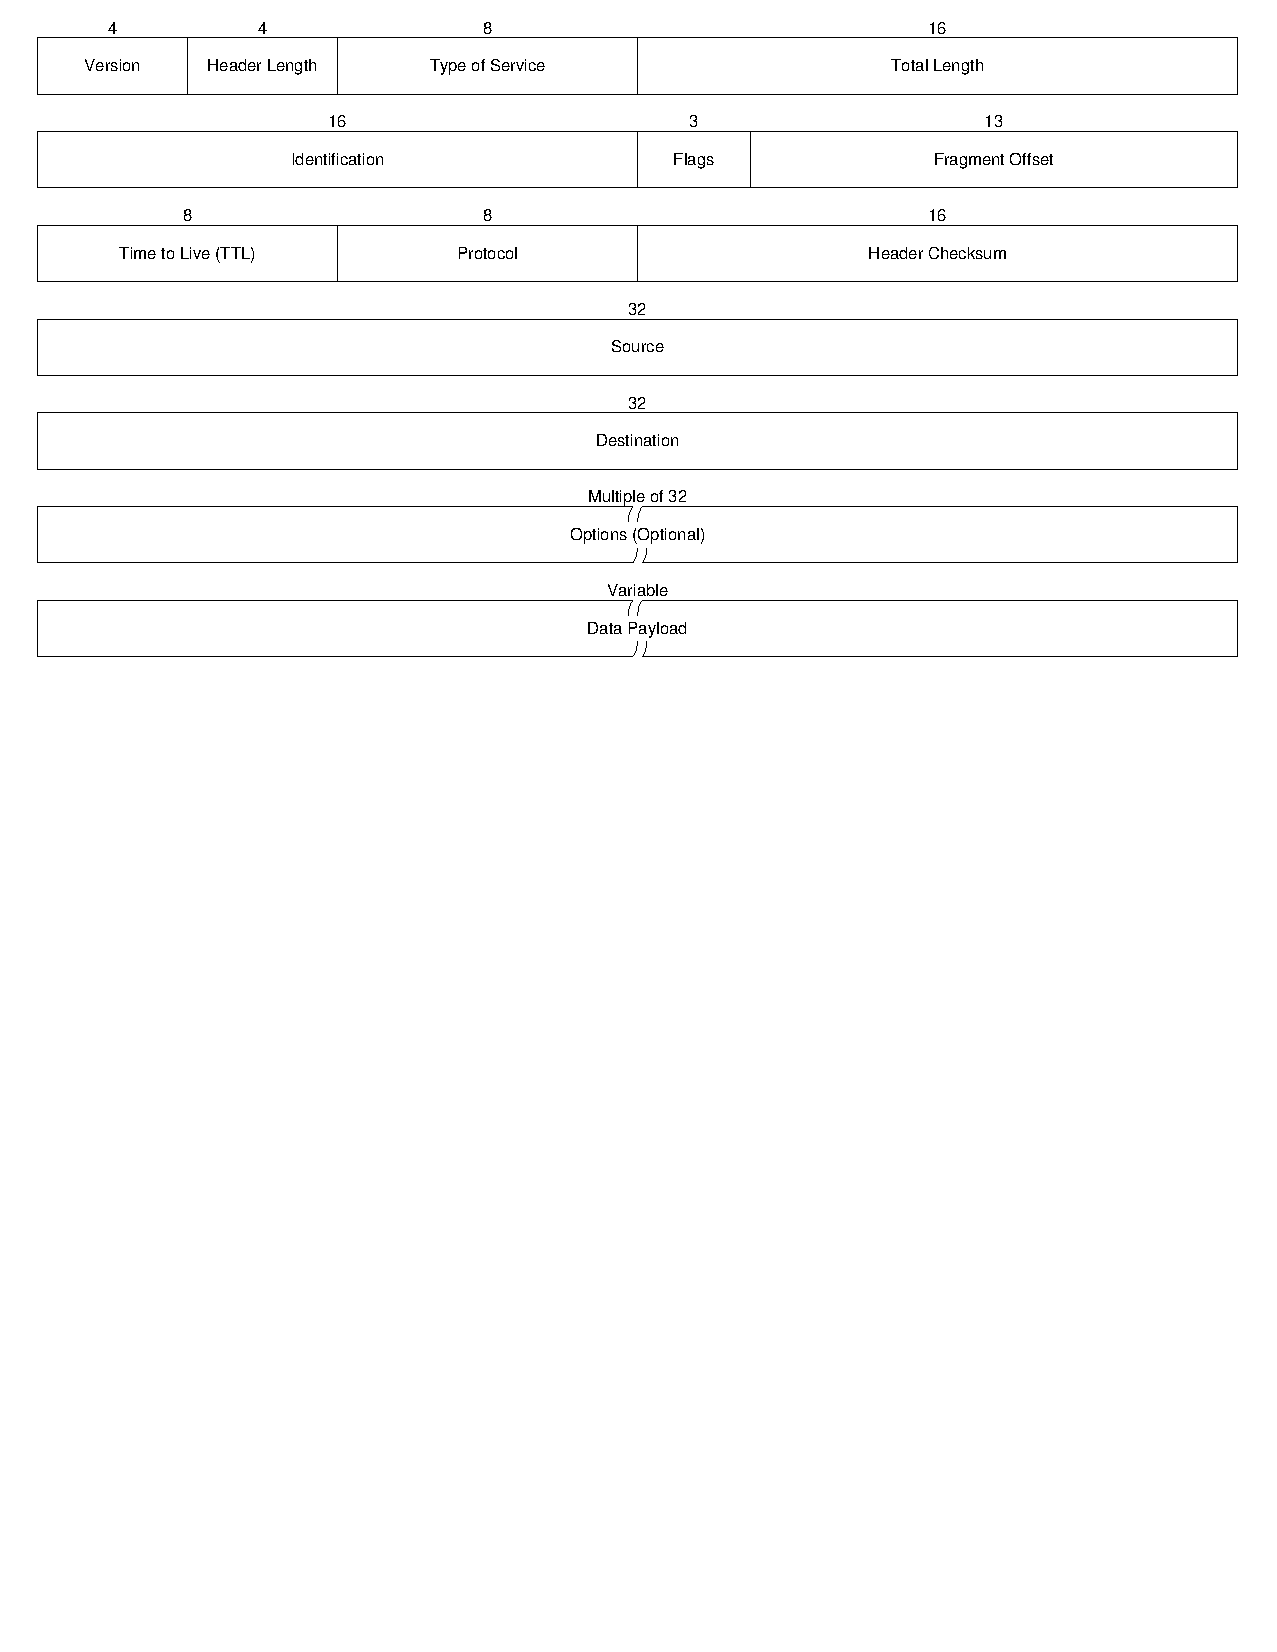
\includegraphics{Protocol/Figures/protocol-ip_header.pdf}
			\caption[IP Header]{IP Header \cite{ref:2005-kozierok-tcpip_guide}}
			\label{fig:protocol:ip_header}
		\end{centering}
	\end{figure}
\end{landscape}

Two protocols are commonly used at the transport layer in TCP/IP: the Transmission Control Protocol (TCP) and the User Datagram Protocol (UDP). TCP provides connection oriented transmission with guaranteed delivery and other services. TCP operations are generally divided into three phases: connection phase, data transfer phase, and termination phase. TCP uses a client/server model, with the server listening on a port. A client that wants to communicate with the server first establishes a connection with the server by talking on the port where the server is listening. After the client and server have finished handshaking, the client can start sending data to the server. After the client is finished sending data, the connection is closed by the client. The header for a TCP packet is shown in Figure \ref{fig:protocol:tcp_header}. The header specifies the source port on the client and the destination port on the server. The sequence number is used to reassemble the fragmented data in the correct order when the packets have been received. The sequence number also indicates that a data packet was not transmitted correctly when a gap in sequence numbers is detected. The acknowledgement number is used to ACK data transfers for guaranteed delivery. TCP allows multiple data packets to be sent before an ACK is required. The amount of data that can be sent before an ACK is required is specified in the window field. The window size can also be used for flow control by setting it to 0. \cite{ref:2005-kozierok-tcpip_guide}

\begin{landscape}
	\begin{figure}[p]
		\begin{centering}
			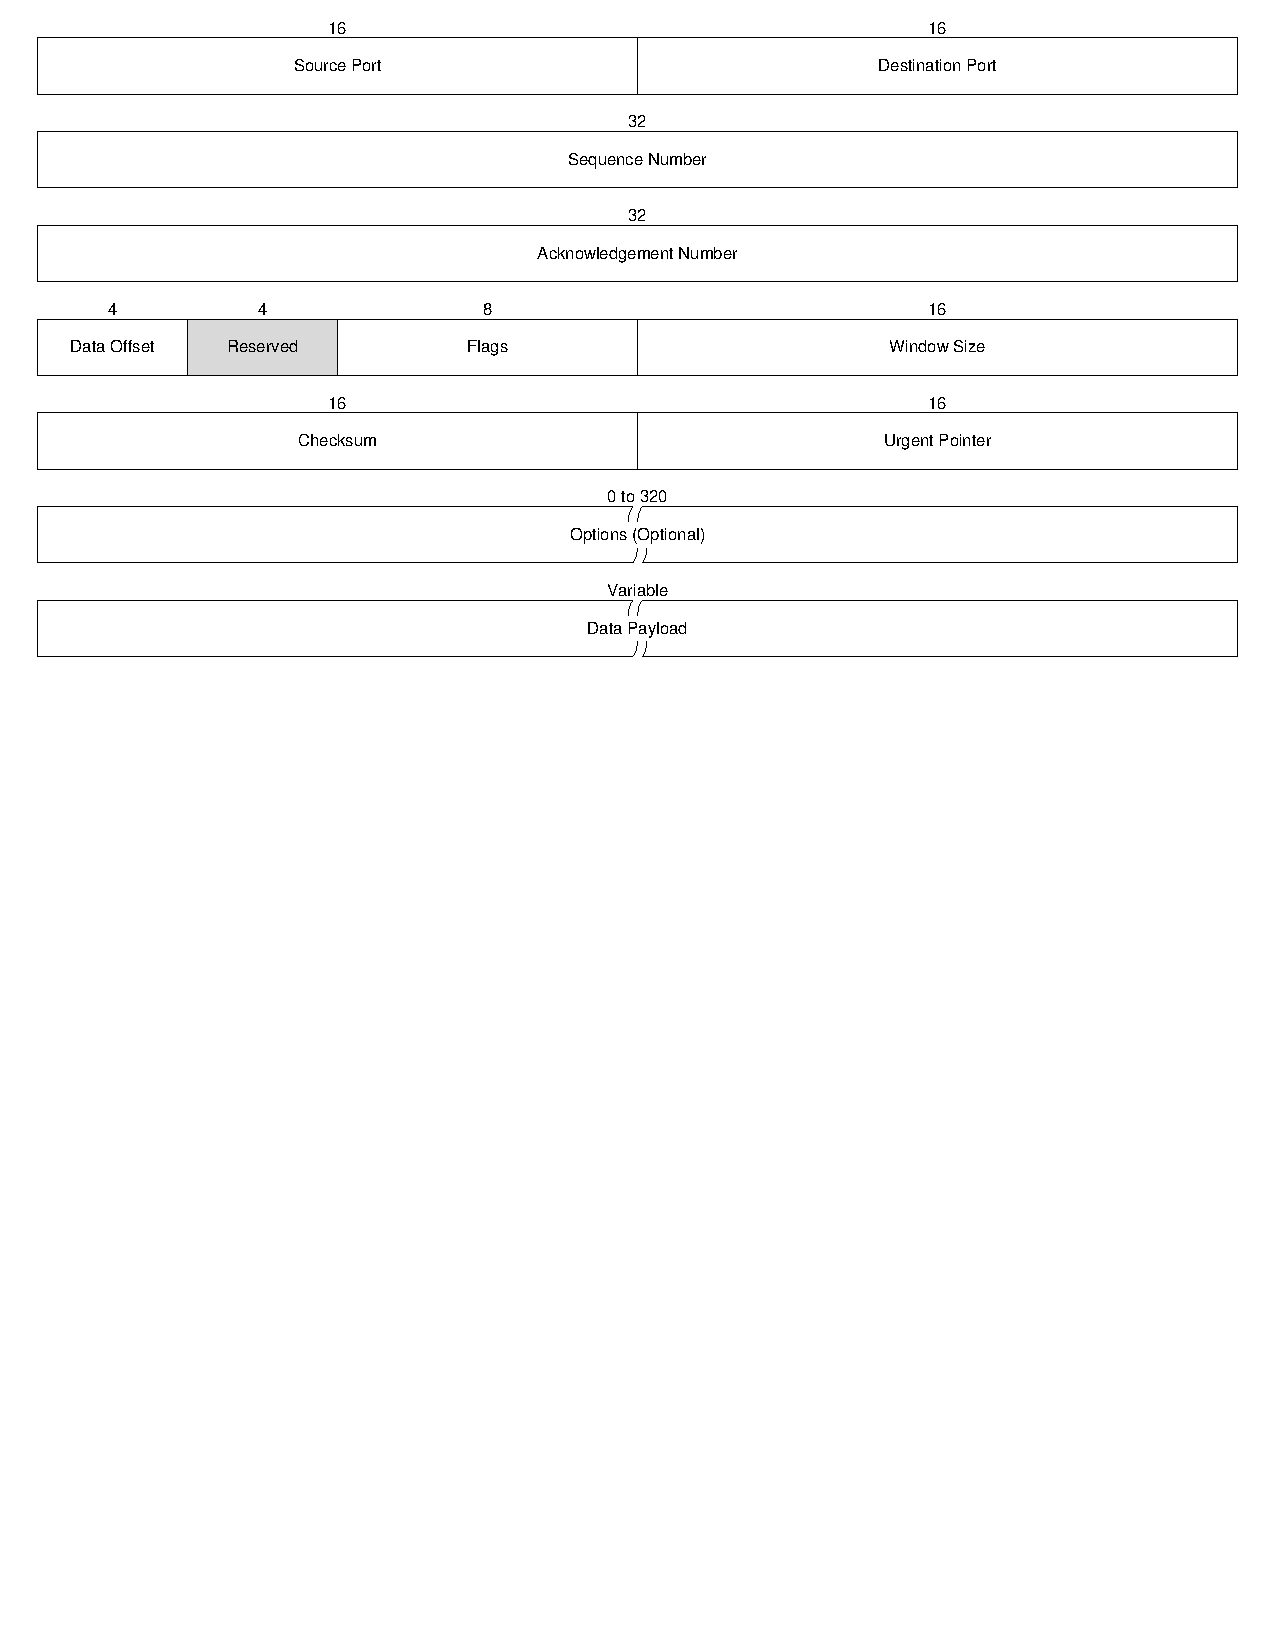
\includegraphics{Protocol/Figures/protocol-tcp_header.pdf}
			\caption[TCP Header]{TCP Header \cite{ref:2005-kozierok-tcpip_guide}}
			\label{fig:protocol:tcp_header}
		\end{centering}
	\end{figure}
\end{landscape}

UDP provides a much more basic (and efficient) connectionless transmission without guaranteed delivery. UDP provides the minimum necessary functionality for a transport level protocol. The maximum length of a UDP packet is, in practice, determined by the underlying network layer, which is 65,507 bytes for IPv4. Because IPv4 does not guarantee delivery, packets can arrive out of order or may not arrive at all, and it is the responsibility of the programmer to handle these situations. The header, shown in Figure \ref{fig:protocol:udp_header}, is 8 bytes long. The short header size, combined with the lack of handshaking/etc. means that UDP has considerably less overhead than TCP, and is ideal for scenarios where some data loss is tolerable, such as streaming media. \cite{ref:2005-kozierok-tcpip_guide}

\begin{landscape}
	\begin{figure}[ptb]
		\begin{centering}
			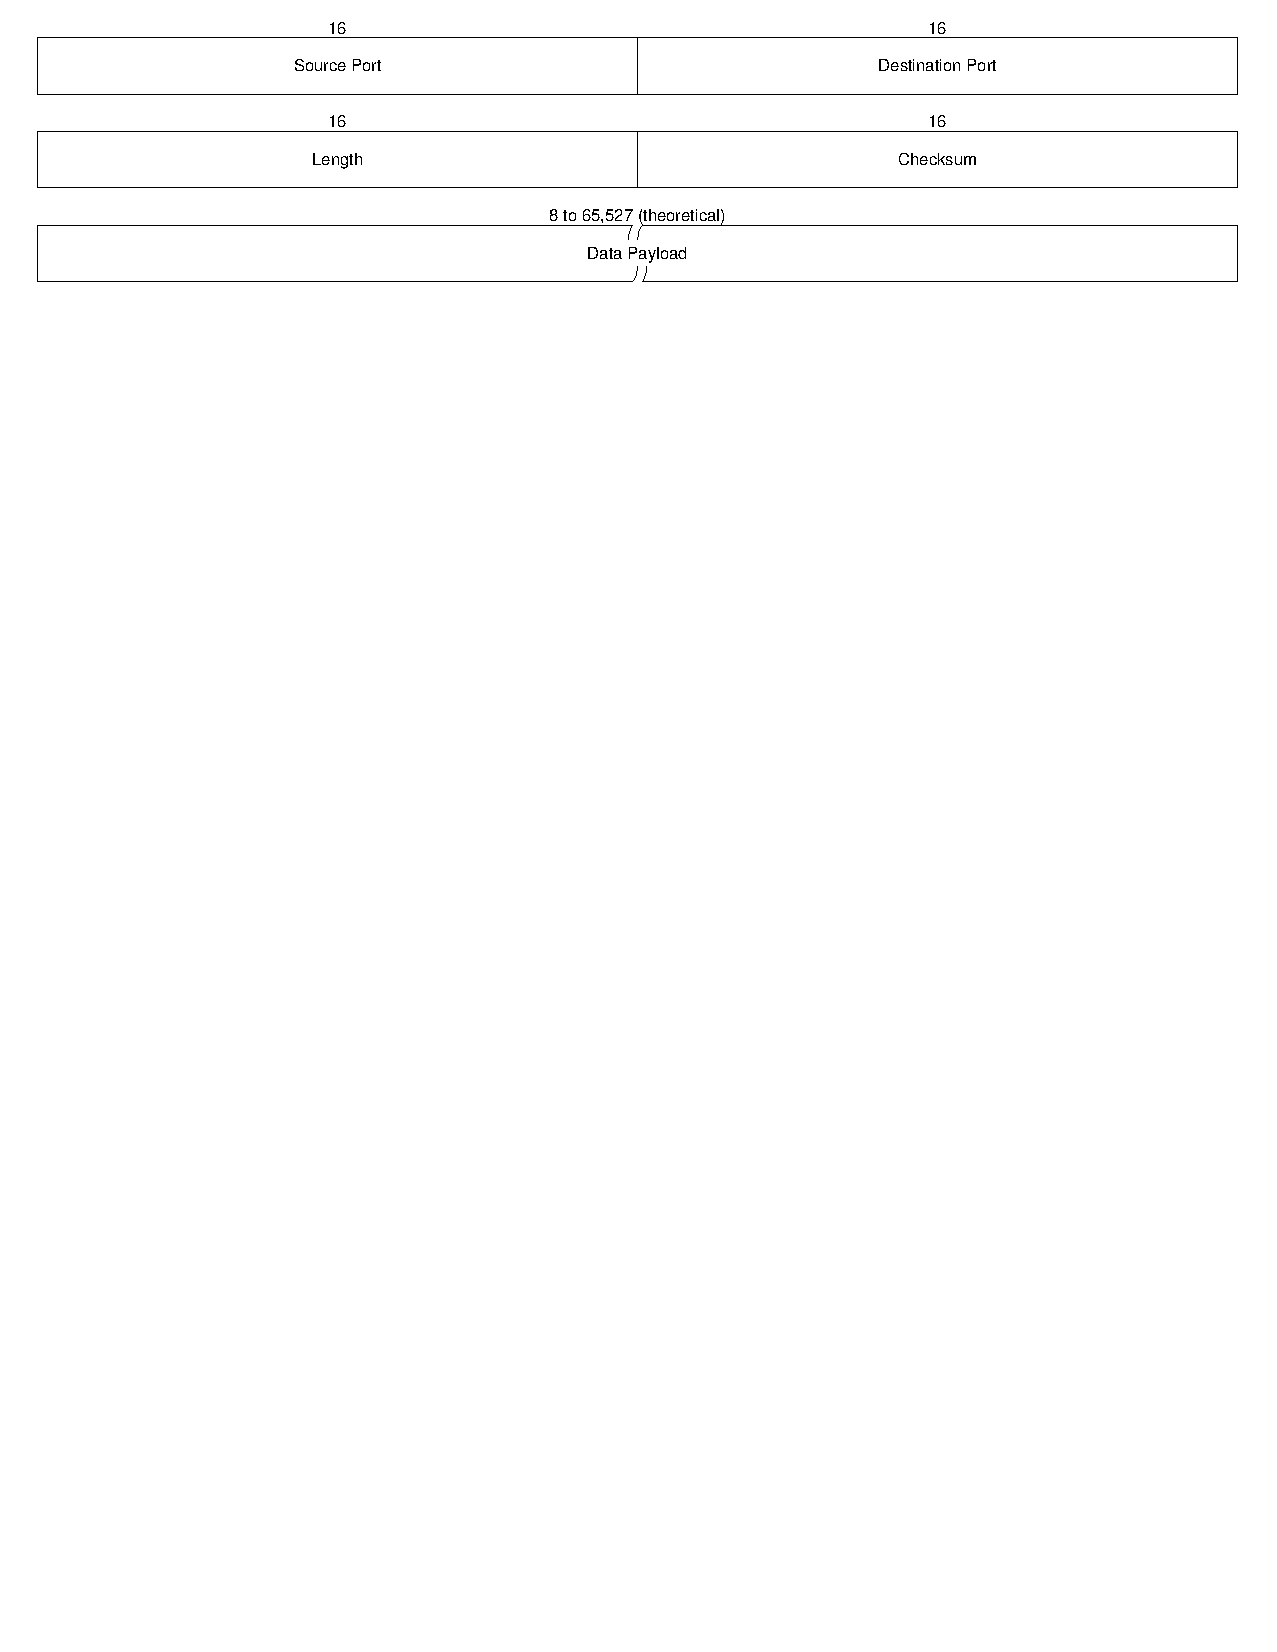
\includegraphics{Protocol/Figures/protocol-udp_header.pdf}
			\caption{UDP Header \cite{ref:2005-kozierok-tcpip_guide}}
			\label{fig:protocol:udp_header}
		\end{centering}
	\end{figure}
\end{landscape}

\subsubsection{RapidIO Overview}\label{sec:protocol:background:protocols:rapidio}

RapidIO was developed specifically for high-end embedded systems and provides physical, data link, and network level communications. RapidIO is a chip-to-chip and board-to-board level interconnect and runs at speeds up to 10 Gbps. RapidIO was designed with the following set of objectives in mind \cite{ref:2005-fuller-rapidio_the_embedded_interconnect}:
\begin{enumerate}
	\item Focus on devices that are ``within the chassis'', i.e. connecting devices in the same system
	\item Limit the impact on software, i.e. do as much in hardware as possible
	\item Confine the protocol overhead so it is as small as possible
	\item Partition the specification into layers
	\item Manage errors in hardware
	\item Limit the silicon footprint
	\item Leverage established I/O driver/receiver technology, i.e. should be implementable in CMOS so that external physical layer hardware is unnecessary
\end{enumerate}
Services are defined at three layers: physical, transport and logical layers. The physical layer defines both a parallel and a serial implementation, handles flow control, low-level error detection/correction, basic packet information, and other services traditionally defined in the data link layer. The transport layer defines the network layer information, including addressing schemes and routing. The logical layer defines several APIs and mechanisms that clients use to communicate. \cite{ref:2005-fuller-rapidio_the_embedded_interconnect}
The serial physical layer uses 8B/10B encoding and supports either one differential pair or four differential pairs (called lanes) that are ``ganged'' together. Data can be transmitted at 1, 2, or 2.5 Gbps per lane. A 3 byte packet header is defined for the serial physical layer and includes ACK and CRC information. The parallel physical layer uses 8- or 16-bit wide LVDS lanes and operates at frequencies of 250 MHz to 1 GHz. The parallel packet is slightly different than the serial variant in specification but contains the same information. The physical layer defines several control packets used for port initialization, error recovery, and flow control for both implementations. \cite{ref:2005-fuller-rapidio_the_embedded_interconnect}
The transport layer is independent of the physical layer and routing implementation. The transport layer header defines three common fields: \emph{Source Address}, \emph{Destination Address}, and \emph{TT} (Transport Type). The 2-bit \emph{TT} field defines the type of transport packet and the other header fields that are included. Currently, \emph{TT}=00 defines 8-bit device IDs, \emph{TT}=01 defines 16-bit device IDs, and \emph{TT}=1x is undefined. The transport layer can optionally add other fields, such as a \emph{Hop Count} field or other management fields. The transport header and logical header are ``interleaved'' in the sense that they are not encapsulated, but rather have their fields defined in a single common specification, as shown in Figure \ref{fig:protocol:rapidio_packets}. This also implies that the logical APIs \emph{must} be used. \cite{ref:2005-fuller-rapidio_the_embedded_interconnect}
The logical layer mechanisms are all defined using a transaction model; communication is always performed in a request-response manner. Request and response packets each have their own basic header definition, with further fields being defined based on the transaction type. The transaction types are grouped according to function into the following groups: I/O, message passing, distributed shared memory, and data streaming. Other protocols, such as PCI, can be transported over RapidIO. When all three layers are taken together, packet overhead can range from 16 to 20 bytes. Typical request and response packets are shown in Figures \ref{fig:protocol:rapidio_packets:request} and \ref{fig:protocol:rapidio_packets:response}, respectively. \cite{ref:2005-fuller-rapidio_the_embedded_interconnect}

\begin{landscape}
	\begin{figure}[ptb]
		\begin{centering}
			\subfigure[Request Packet]
			{
				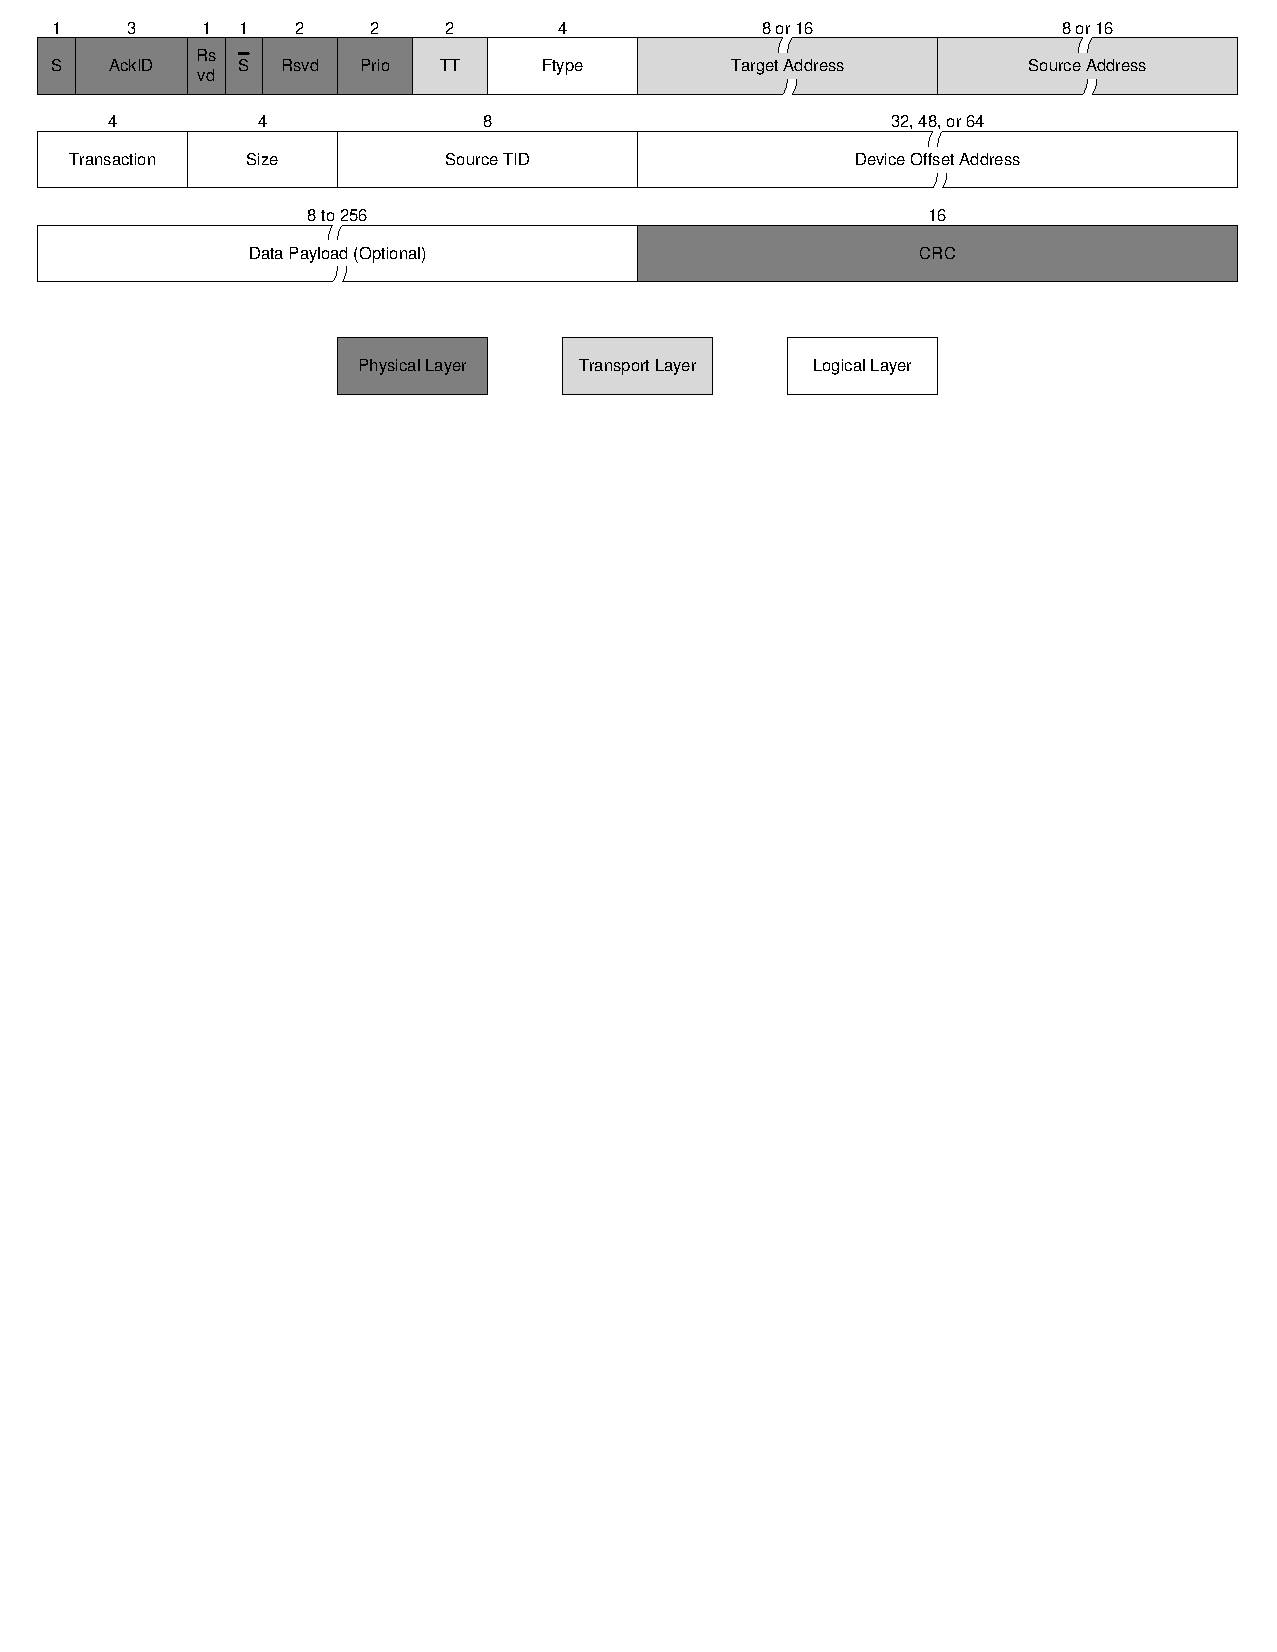
\includegraphics[scale=0.9]{Protocol/Figures/protocol-rapidio_request_header.pdf}
				\label{fig:protocol:rapidio_packets:request}
			}
			\subfigure[Response Packet]
			{
				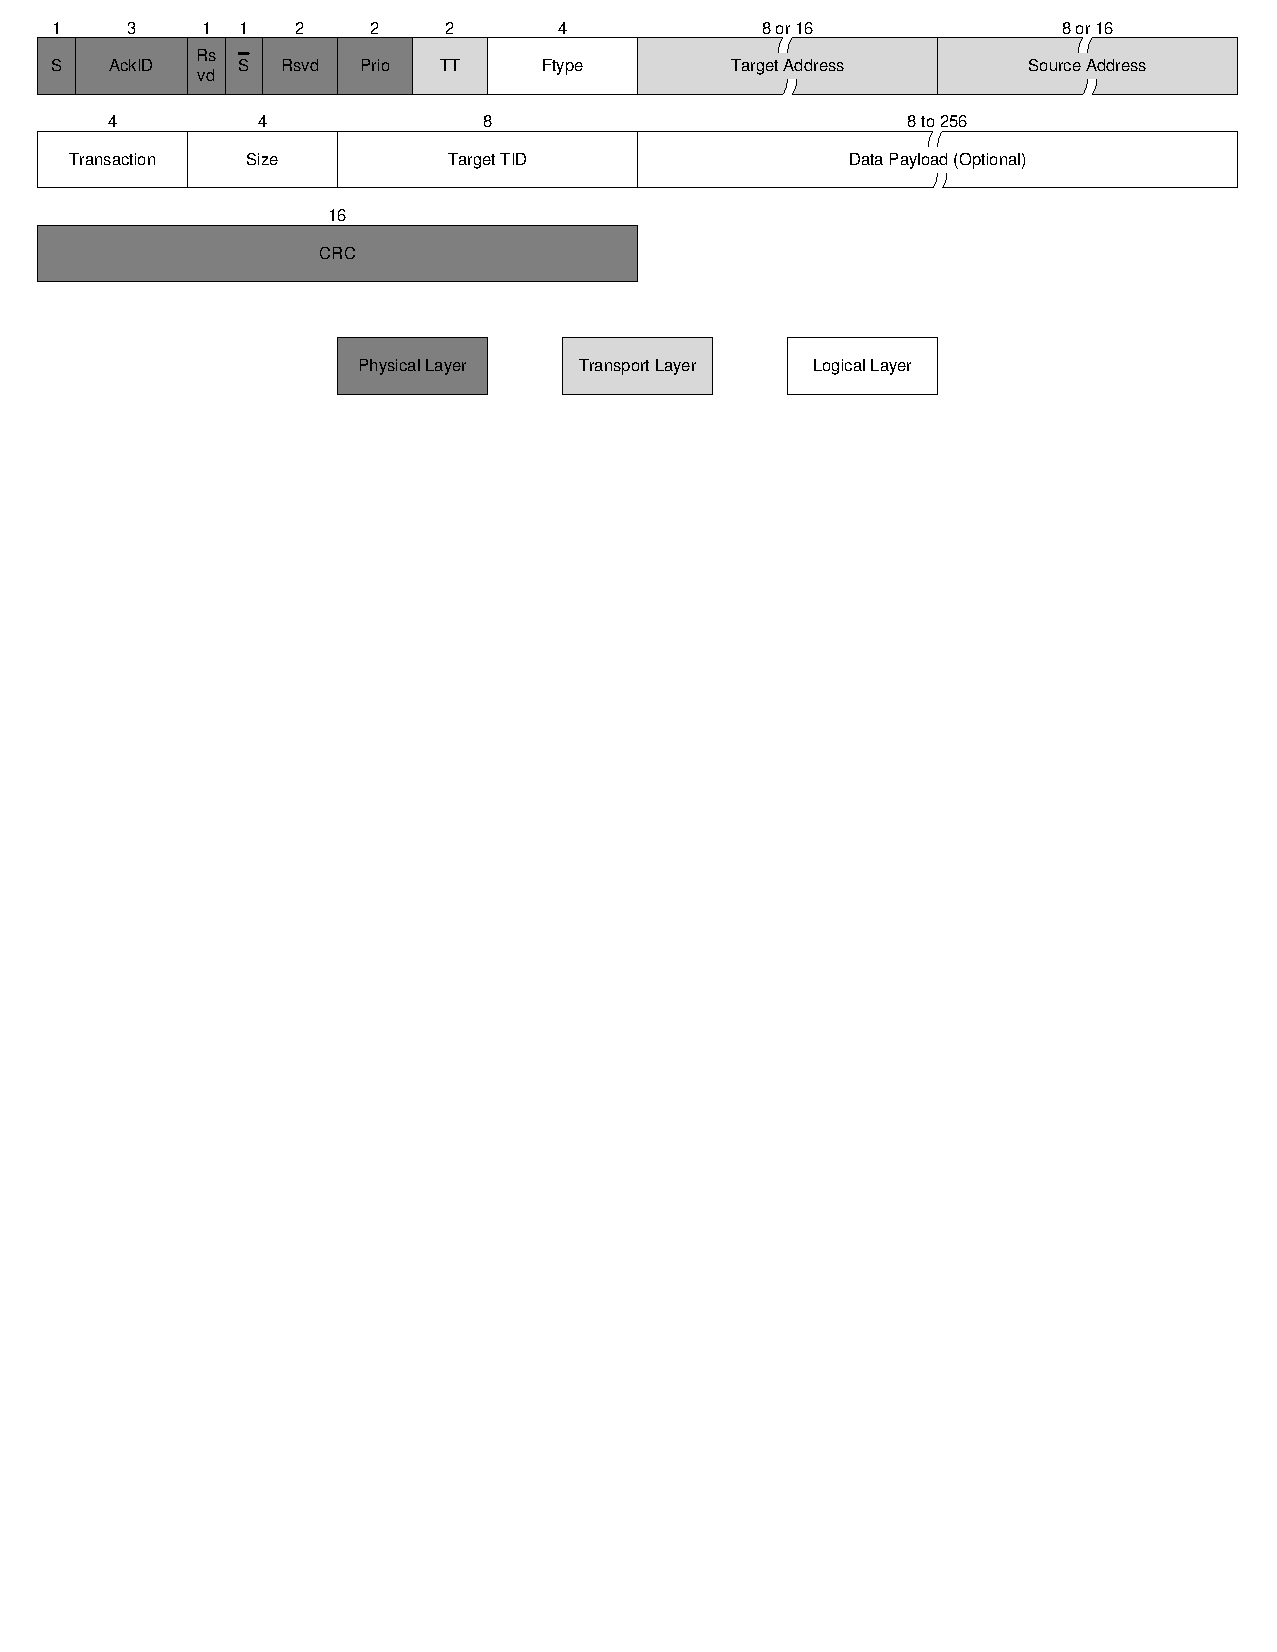
\includegraphics[scale=0.9]{Protocol/Figures/protocol-rapidio_response_header.pdf}
				\label{fig:protocol:rapidio_packets:response}
			}
			\caption{Typical RapidIO request and response packets}
			\label{fig:protocol:rapidio_packets}
		\end{centering}
	\end{figure}
\end{landscape}

\subsection{Communication Faults}\label{sec:protocol:introduction:communication_faults}

Four primary faults can occur at the network layer: dead-lock, live-lock, starvation, and path cycles. These faults can cause a communication system to become completely unresponsive and must be avoided at all costs.

Dead-lock is a situation that happens when packets get stuck because they are requesting resources that other packets currently have reserved. An example is shown in Figure \ref{fig:protocol:dead_lock}. In this scenario, all buffers are full (each buffer element has its destination listed). The packets at node 1 can't move on to node 2 because the packets at node 2 are occupying all available buffers. Node 2 can't move on to node 3 for the same reason, and so forth.

\begin{figure}[ptb]
	\begin{centering}
		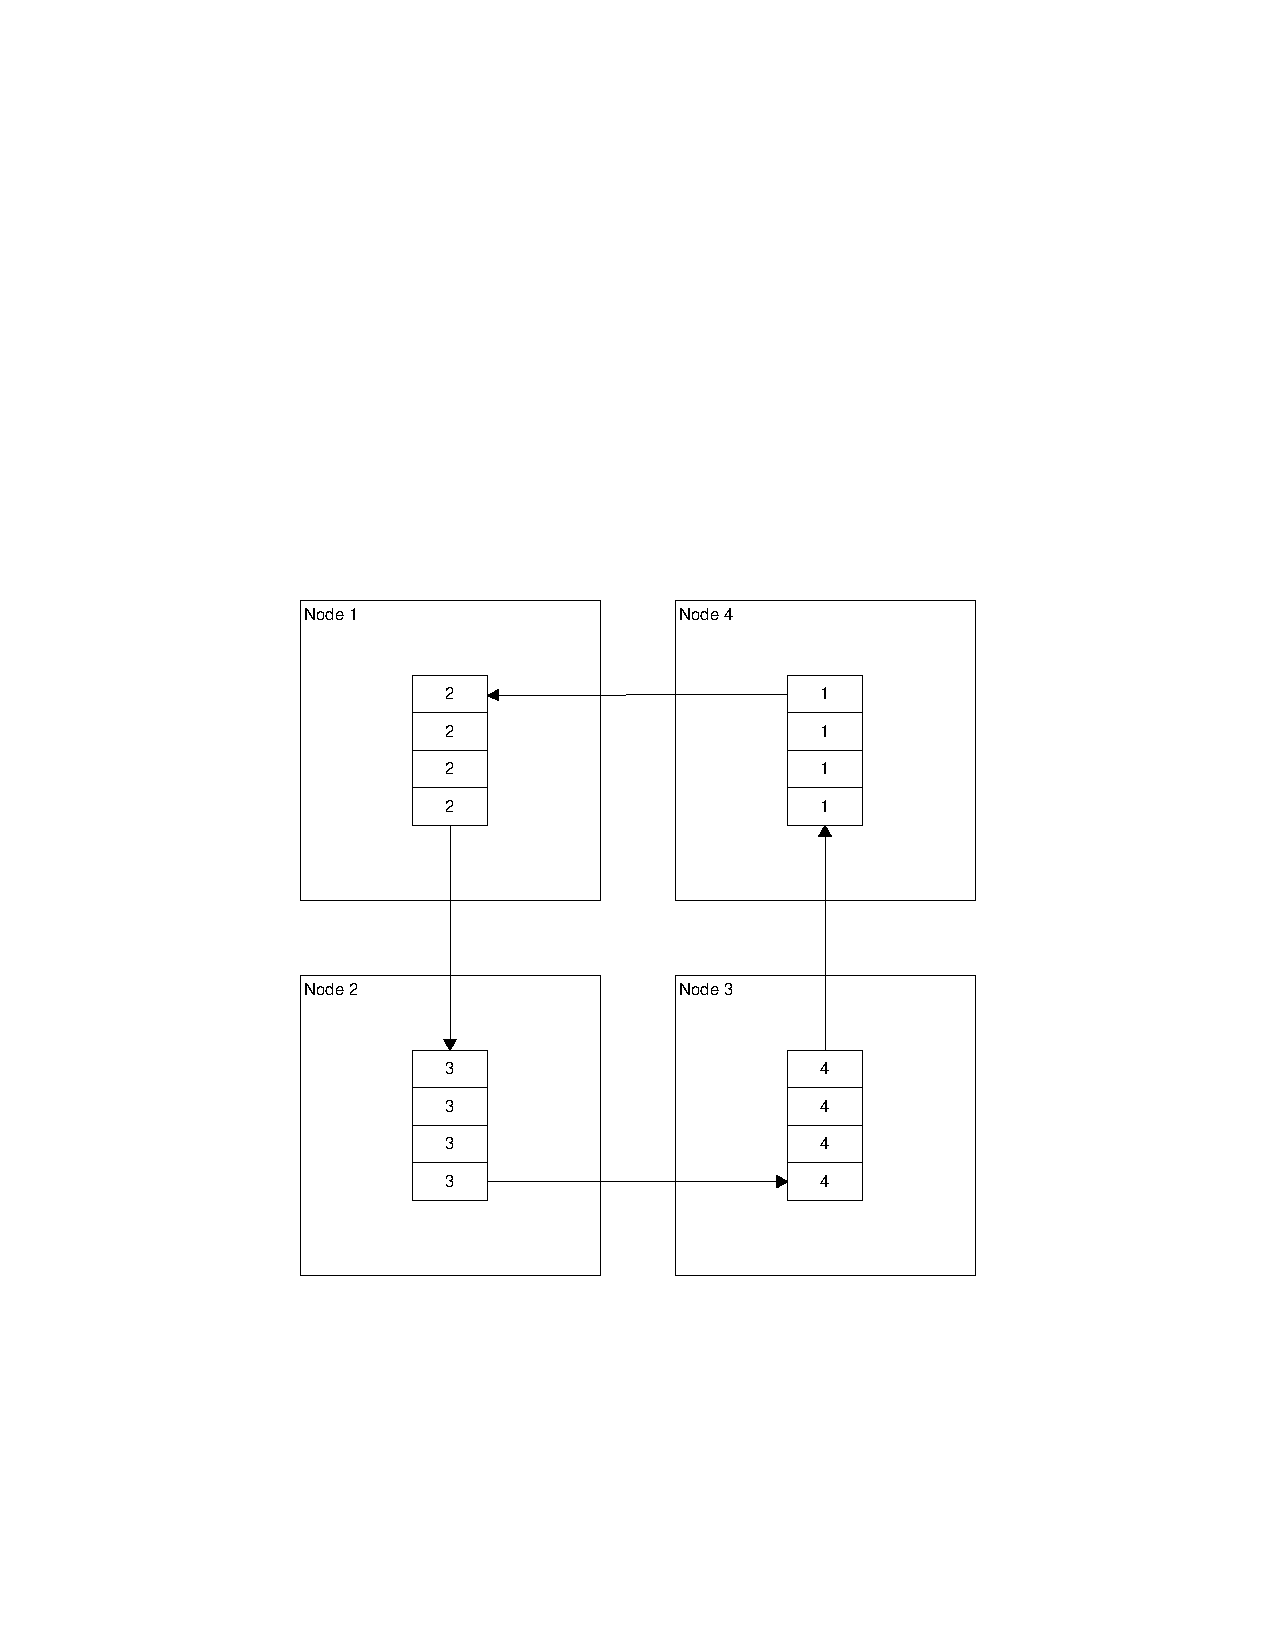
\includegraphics[scale=0.75]{Protocol/Figures/protocol-dead_lock.pdf}
		\caption{Example dead-locked fault}
		\label{fig:protocol:dead_lock}
	\end{centering}
\end{figure}

Live-lock is similar to dead-lock, except that packets are still moving in the system. A common example of live-lock is when two nodes try to transmit at the same time and collide. Each node backs of waits the same amount of time and tries again, and collides again, and they keep going on like this forever.

Starvation occurs when a packet is prevented from acquiring resources indefinitely because other resources continually acquire all available resources first. An example is shown in Figure \ref{fig:protocol:starvation} where node 4 is blocked from sending a priority 2 message to node 1 because node 3 is streaming higher priority 3 messages to node 1.

\begin{figure}[ptb]
	\begin{centering}
		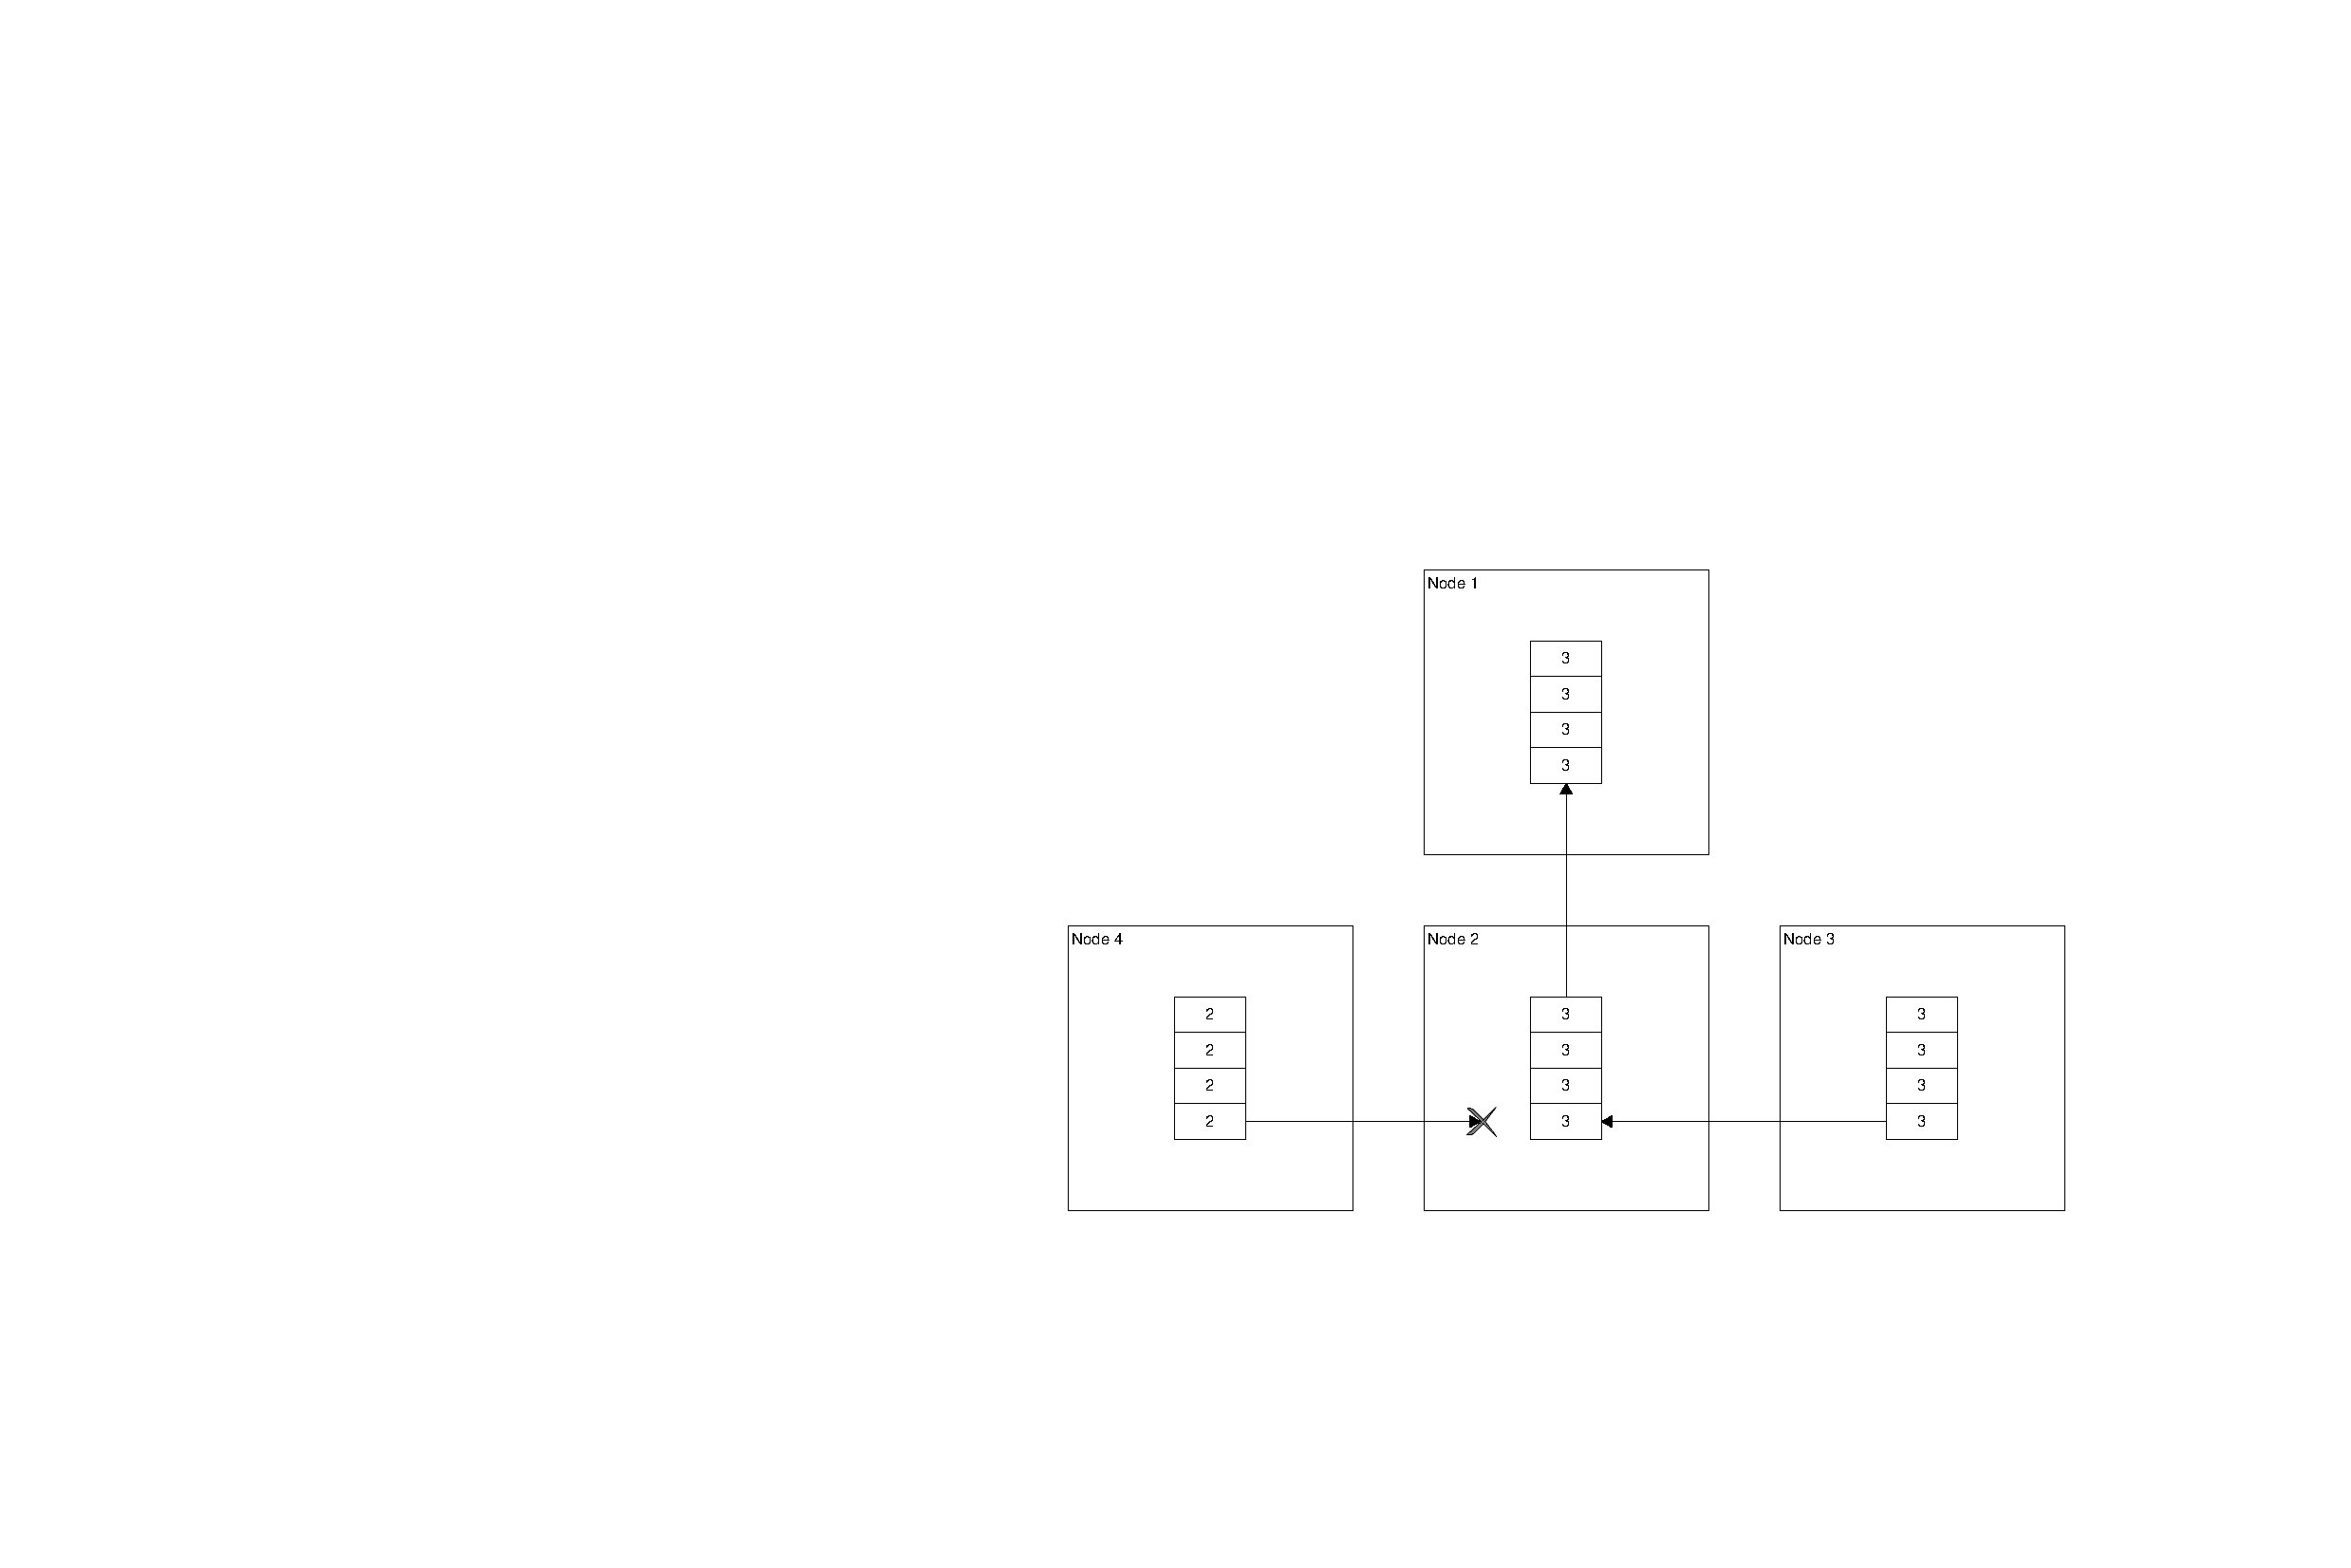
\includegraphics[scale=0.75]{Protocol/Figures/protocol-starvation.pdf}
		\caption{Example starvation fault}
		\label{fig:protocol:starvation}
	\end{centering}
\end{figure}

Path cycles can occur when the routing algorithm is allowed to take non-minimal paths, i.e. does not have to take the shortest path from A to B. A path cycle occurs when a packet continuously travels in a circle without reaching its destination. This is possible in all adaptive routing algorithms, and in some oblivious routing algorithms, unless explicit measures are taken to prevent it.

\section{Objectives}\label{sec:protocol:objectives}

The protocol must meet the following criteria: 
\begin{enumerate}
	\item Supports ``end-to-end'' transmissions
	\item Provides dynamic and self-configuring addressing
	\item Provides error checking
	\item Proper complexity for mainstream embedded systems
	\item Fault tolerance
\end{enumerate}
Most of these criteria ensure that the system is easy to use by application developers. End-to-end transmissions, i.e. transmissions between nodes that are not directly connected, must be supported and be transparent to the application developer. Error checking is vital in any communications system, and this one should be no different. The complexity of the protocol must be proportional to the complexity of embedded systems. In other words, it needs to support features expected of a mainstream system, without going overboard and re-implementing TCP/IP. The system must be fault tolerant with respect to dead-lock, live-lock, and starvation\footnote{It is the responsibility of the routing algorithm to ensure path cycles are not encountered}.

\section{Methodology} \label{sec:protocol:methodology}

The current protocols that exist are eschewed in favor of a custom protocol. TCP/IP over Ethernet is simply a poor fit for embedded systems: the \emph{minimum} combined header size for a UDP based packet is 50 bytes, and is 62 bytes for a TCP based packet. RapidIO has much smaller packets, but can still be variable in length. Variable length packet headers can certainly be more flexible than fixed length, but the processing firmware is more complex as a result. RapidIO also has a plethora of different header definitions, which makes the protocol stack considerably more complex. Given the target application of mainstream embedded processors that are responsible for the protocol \emph{and} application, a fixed packet header of very small length is more appropriate.

\subsection{Custom Protocol Concepts}\label{sec:protocol:methodology:concepts}

A custom protocol has been created that borrows elements from both RapidIO (such as small header size) and TCP/IP over Ethernet (such as packet identification), while trying to keep everything simpler than either protocol. One means to keep the protocol simple is to combine all headers above the data link layer into a single packet, i.e. only one packet definition exists instead of packets inside of packets, like TCP inside of IP. Another way that the protocol is kept simple is by using a ``root'' node with a pre-determined address to handle addressing and global management instead of using a distributed approach. This simplifies the address acquisition process considerably, because a node requesting an address does not have to first send out ``discover'' packets to find out where the root node is. Using a root node also simplifies the creation of the routing table, described in Chapter \ref{sec:routing}. The downside to using a root node is that if something happens to the root node, then the entire system is brought down. This is deemed as acceptable for this application because a node disappearing in an embedded system is more than likely a hardware failure, and thus is symptomatic of greater problems. This mechanism satisfies the addressing objective and also helps to satisfy the complexity objective.

Pipelined circuit switching is used in the system because it is reliable and eliminates the need to buffer complete packets in a node other than the destination node, while keeping the firmware simple. PCS is only used for data transfers because single flits are never broken up or buffered, and a header is exactly one flit. The ``probe'' packet would consist of the entire control packet, so there would be no data to transfer in this case. This is the key point in realizing fault tolerance for dead-lock and live-lock. When a channel is reserved for a transfer, dead-lock, live-lock, and starvation cannot happen \emph{by definition}. This means that probe packets and header packets are the only transfers that can still fault. The use of virtual channels, as described in Chapter \ref{sec:spi}, avoids dead-lock and live-lock for header/probe packets. Starvation is avoided by not using a priority-based system. All flits are queued in FIFO order, which means that packets are serviced on a first-come, first-serve basis, guaranteeing that packets will be processed eventually. This trade-off is deemed acceptable because embedded networks just do not have the variety of traffic that computer networks do. To help prevent path cycles, the entire path the packet will take in the network is determined in advance and stored in the packet header. These mechanisms satisfy the fault tolerance objective.

\subsection{Packet Header Format}\label{sec:protocol:methodology:header_format}

 A packet header has been designed that is simple yet flexible. The full packet header is shown in Figure \ref{fig:protocol:packet_header}.

\begin{landscape}
	\begin{figure}[p]
		\begin{centering}
			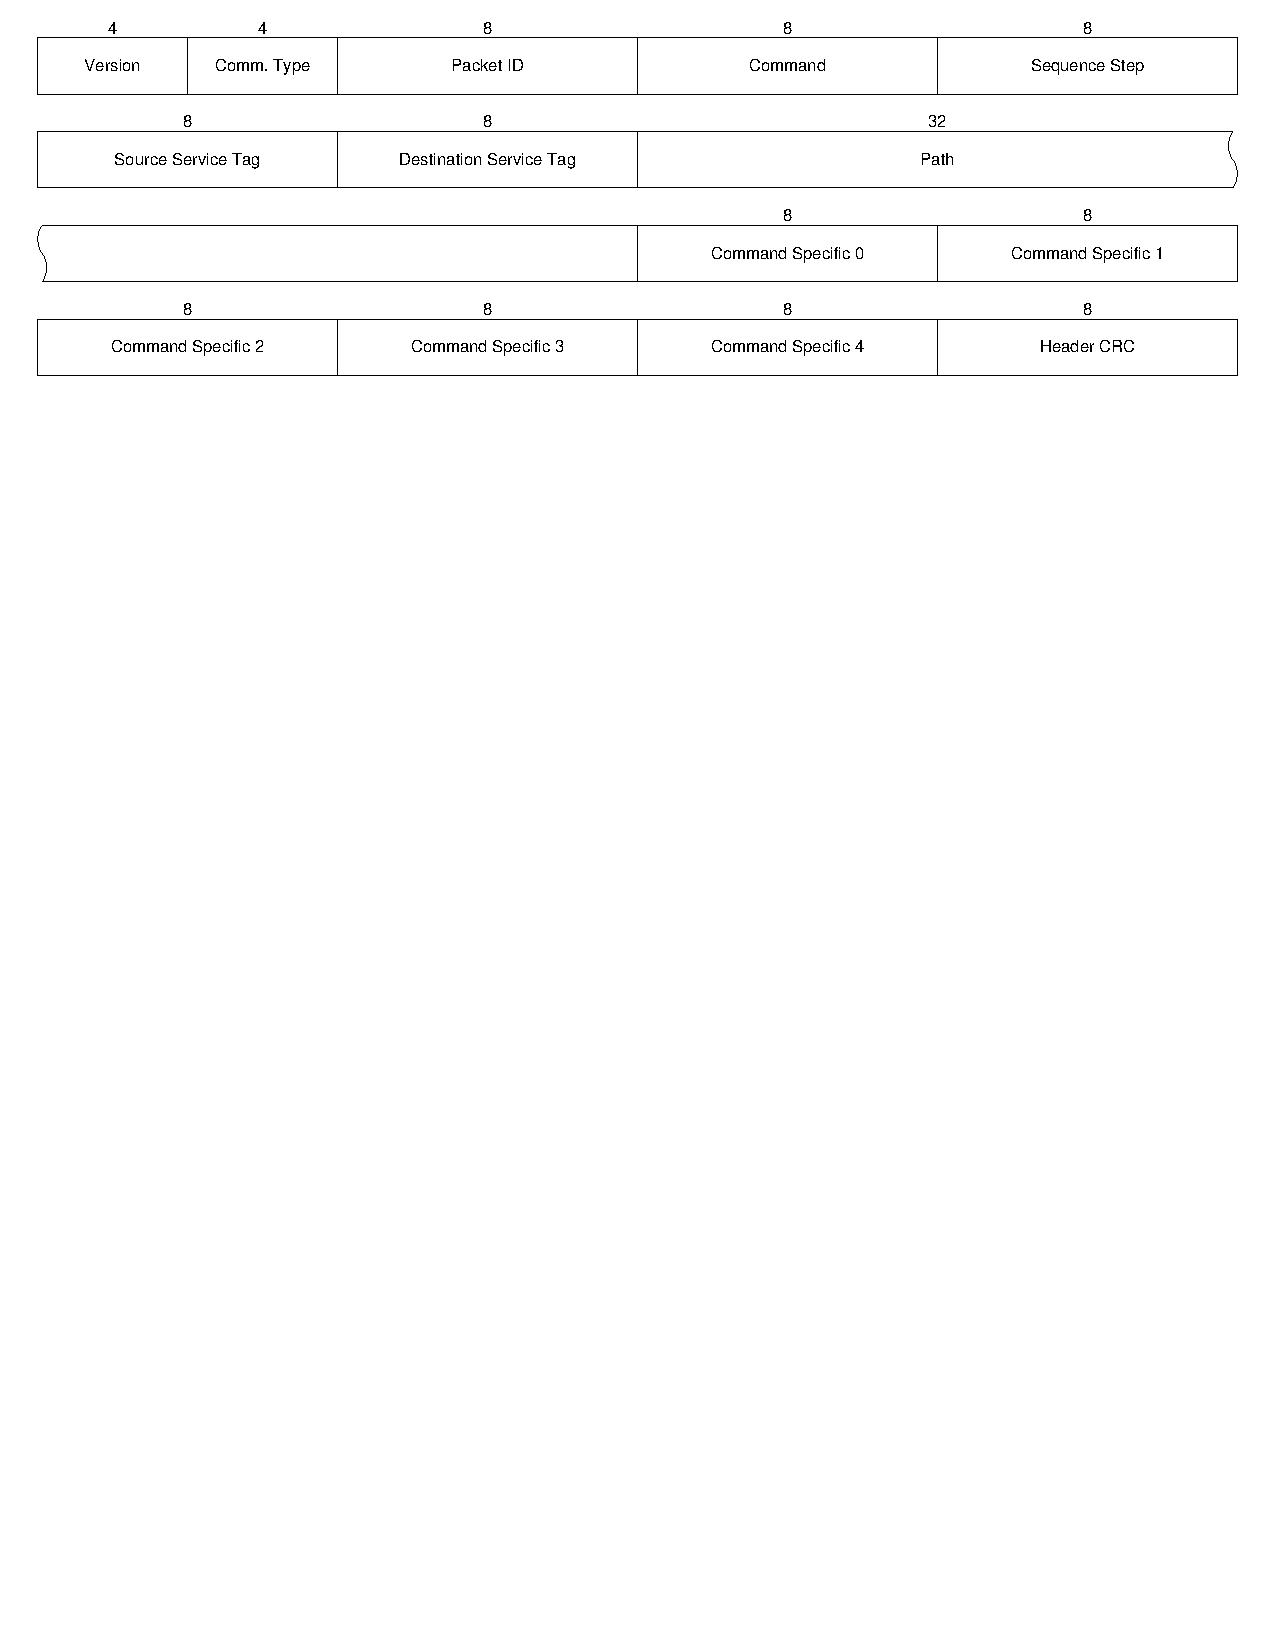
\includegraphics{Protocol/Figures/protocol-packet_header.pdf}
			\caption{Packet Header}
			\label{fig:protocol:packet_header}
		\end{centering}
	\end{figure}
\end{landscape}

The version field specifies the protocol version of the header, although in practice it basically just serves as a training sequence because the current version is still version 1. The communication type field enumerates the communication type for this packet. The header supports unicast, broadcast, multicast, and a fourth type of communication called addressless communication, which is used for data-link layer communications. The packet ID serves as an identifier for the packet and is used for data transfer lookups, resource reservations, and the like. The field is only 8-bits, so it can't identify every packet over the entire duration of program execution, but can locally identify the packet within the temporal locality of commands.

In TCP/IP, nested layers are used to allow different types of communication to utilize common lower layers. RapidIO utilizes a combination of nested layers and multiple packet formats to achieve similar flexibility. To achieve a similar end, the custom protocol utilizes ``commands'' that are enumerated in the command field that specify the packet's purpose (the current list of commands are in Table \ref{tab:protocol:commands}). Each command has an associated set of ``sequence steps,'' enumerated in the sequence step field, which are used to store the command state in the packet itself, thus eliminating the need to store state in nodes. All packets involved in the transfer have the same command and packet ID, which ``links'' the packets together. When a node receives a packet, the next step is determined by the previous step only. For example, a data transfer consists of the following sequence steps: path reservation, reservation ACK, data transfer, and data transfer ACK. A node does not have to remember that a path reservation request was sent in order to complete the rest of the data transfer command, because the reservation ACK sequence step packet alone will tell us that the data should be sent next. 

Source and destination service tags are used for routing data transfers within a node and serve the same purpose as ports in TCP and UDP. They differ from ports in that tags are more abstract, and they directly enumerate a type of service. In contrast, port 80 in TCP typically indicates a web server, but nothing stops an administrator from using port 21 (normally used for FTP) instead. The Command specific fields are used for information that is not common across all commands. 

The complete path that the node will take through the system is calculated at the source and stored in the header. The path is compressed and stored in a single 32-bit integer, with each node being represented by a 4-bit number. This does impose a limit of 16 nodes in the system and a maximum path length of 8, but this is deemed acceptable for the current application. This is an area for further improvement in the future, however, and is discussed in Section \ref{sec:protocol:future_work}.

\subsection{Commands}\label{sec:protocol:methodology:commands}

The available commands are intended to bridge the middle layers, but at the same time they are not application specific. Commands available must fulfill all of the features expected of the protocol. This means that commands must be available that handle addressing, routing table distribution, communication failure handling, and transfers for applications. The list of commands is shown in Table \ref{tab:protocol:commands}.

\begin{table}
	\begin{center}
		\setlength{\extrarowheight}{1.5pt}
		\caption{List of Commands}
		\vspace{0.1cm}
		\begin{tabular}{|l|l|}
			\hline
			\textbf{Command} & \textbf{Description} \\
			\hline
			\hline
			Discover Neighbors & Probe links to see who, if anyone, is attached \\
			& to that link \\
			\hline
			Request Address & Request an address from the root node \\
			\hline
			Report Neighbors & Report neighbors to the root node \\
			\hline
			Routing Table Available & A new routing table is available \\
			\hline
			Request Routing Table & Request the routing table from the root \\
			\hline
			Communication Failure & A node stopped communicating (sent to root to \\
			& regenerate routing table) \\
			\hline
			Data Transfer & Transfer generic data payload \\
			\hline
			Application Control & Application-specific control packet \\
			\hline
		\end{tabular}
		\label{tab:protocol:commands}
	\end{center}
\end{table}

\subsubsection{Discover Neighbors} \label{ref:protocol:methodology:commands:discover_neighbors}

The discover neighbors command plays a pivotal role in establishing basic information for use by other commands. Knowing whether or not a neighbor is present a) identifies when and via whom an address can be requested and b) indicates when a neighbor has disappeared. The list of sequence steps are shown in Table \ref{tab:protocol:discover_neighbors}, and the flow diagram showing the progression of the command is shown in Figure \ref{fig:protocol:discover_neighbors}.
\begin{table}
	\begin{center}
		\setlength{\extrarowheight}{1.5pt}
		\caption{Sequence Steps for the Discover Neighbors Command}
		\vspace{0.1cm}
		\begin{tabular}{|l|l|}
			\hline
			\textbf{Sequence Step} & \textbf{Description} \\
			\hline
			\hline
			Request Neighbor Info & Request address and if they are the root \\
			\hline
			Neighbor Response & Send requested information \\
			\hline
			Error & The request could not be completed \\
			\hline
		\end{tabular}
		\label{tab:protocol:discover_neighbors}
	\end{center}
\end{table}

\begin{figure}[ptb]
	\begin{centering}
		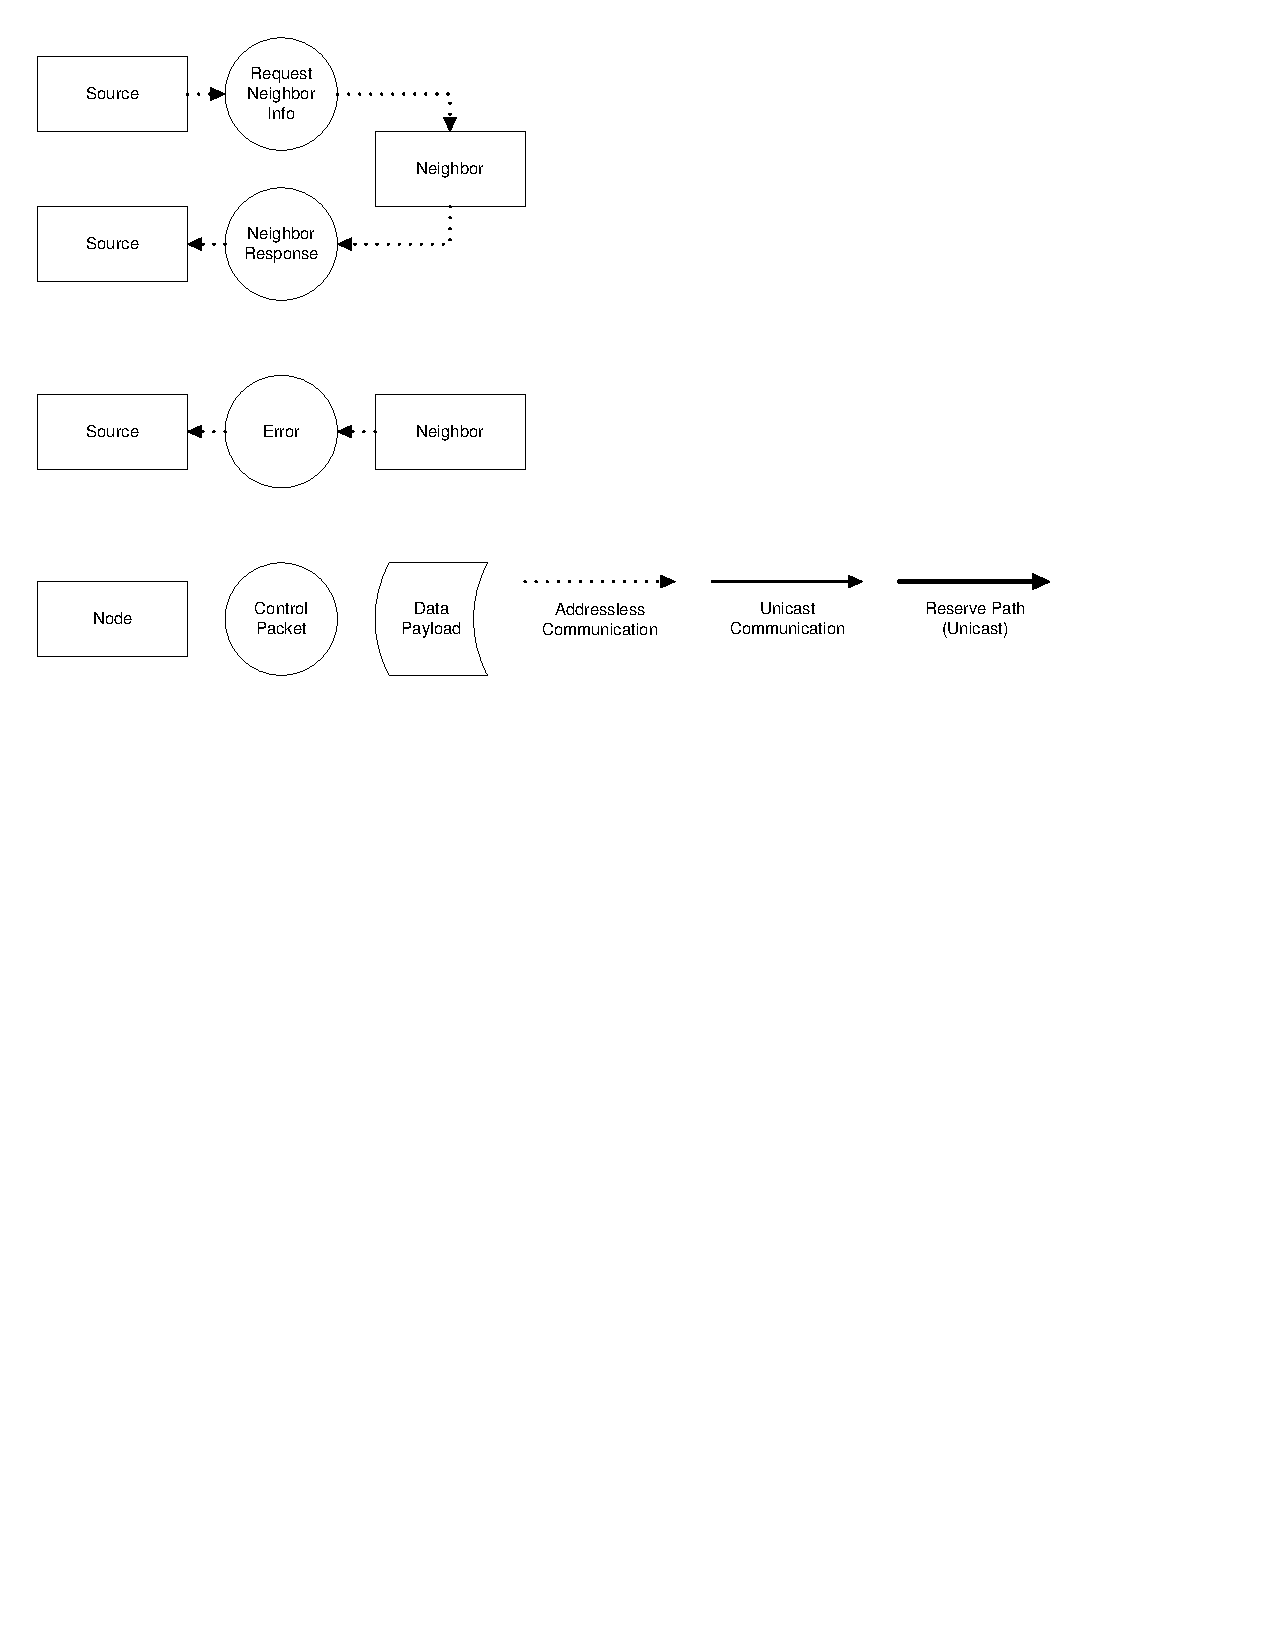
\includegraphics{Protocol/Figures/protocol-discover_neighbors.pdf}
		\caption{Flow diagram for the Discover Neighbors Command}
		\label{fig:protocol:discover_neighbors}
	\end{centering}
\end{figure}

\subsubsection{Request Address}\label{ref:protocol:methodology:commands:request_address}

When a node powers up, it does not have any means of identifying itself until it is assigned an address from the root node. In comparison, computer network interface cards have a unique hardware address, called the Media Access Control (MAC) address, that allows them to communicate with other local computers until it receives an IP address from a server. A proxy mechanism has been created because no hard-wired address or other method of identifying the node exists. When a node powers up, it checks to see if any of its neighbors have an address via the Discover Neighbors command. The first neighbor found with an address acts as a proxy and requests the address on behalf of the node, unless one of the neighbors is the root and the node can communicate directly. This process leads to a cascade where all addresses are eventually assigned. When a node has an address, it can then use traditional communication types like unicast. The list of sequence steps are shown in Table \ref{tab:protocol:request_address}, and the flow diagram is shown in Figure \ref{fig:protocol:request_address}.

\begin{table}
	\begin{center}
		\setlength{\extrarowheight}{1.5pt}
		\caption{Sequence Steps for the Request Address Command}
		\vspace{0.1cm}
		\begin{tabular}{|l|l|}
			\hline
			\textbf{Sequence Step} & \textbf{Description} \\
			\hline
			\hline
			Request Address & Request an address from the root \\
			\hline
			Request Address Forward & Forward the request to the root on behalf of a neighbor \\
			\hline
			Grant Address Forward & Send the requested address to the proxy neighbor \\
			\hline
			Grant Address & Send the address to the node requesting it \\
			\hline
			Error & The request could not be completed \\
			\hline
		\end{tabular}
		\label{tab:protocol:request_address}
	\end{center}
\end{table}

\begin{figure}[ptb]
	\begin{centering}
		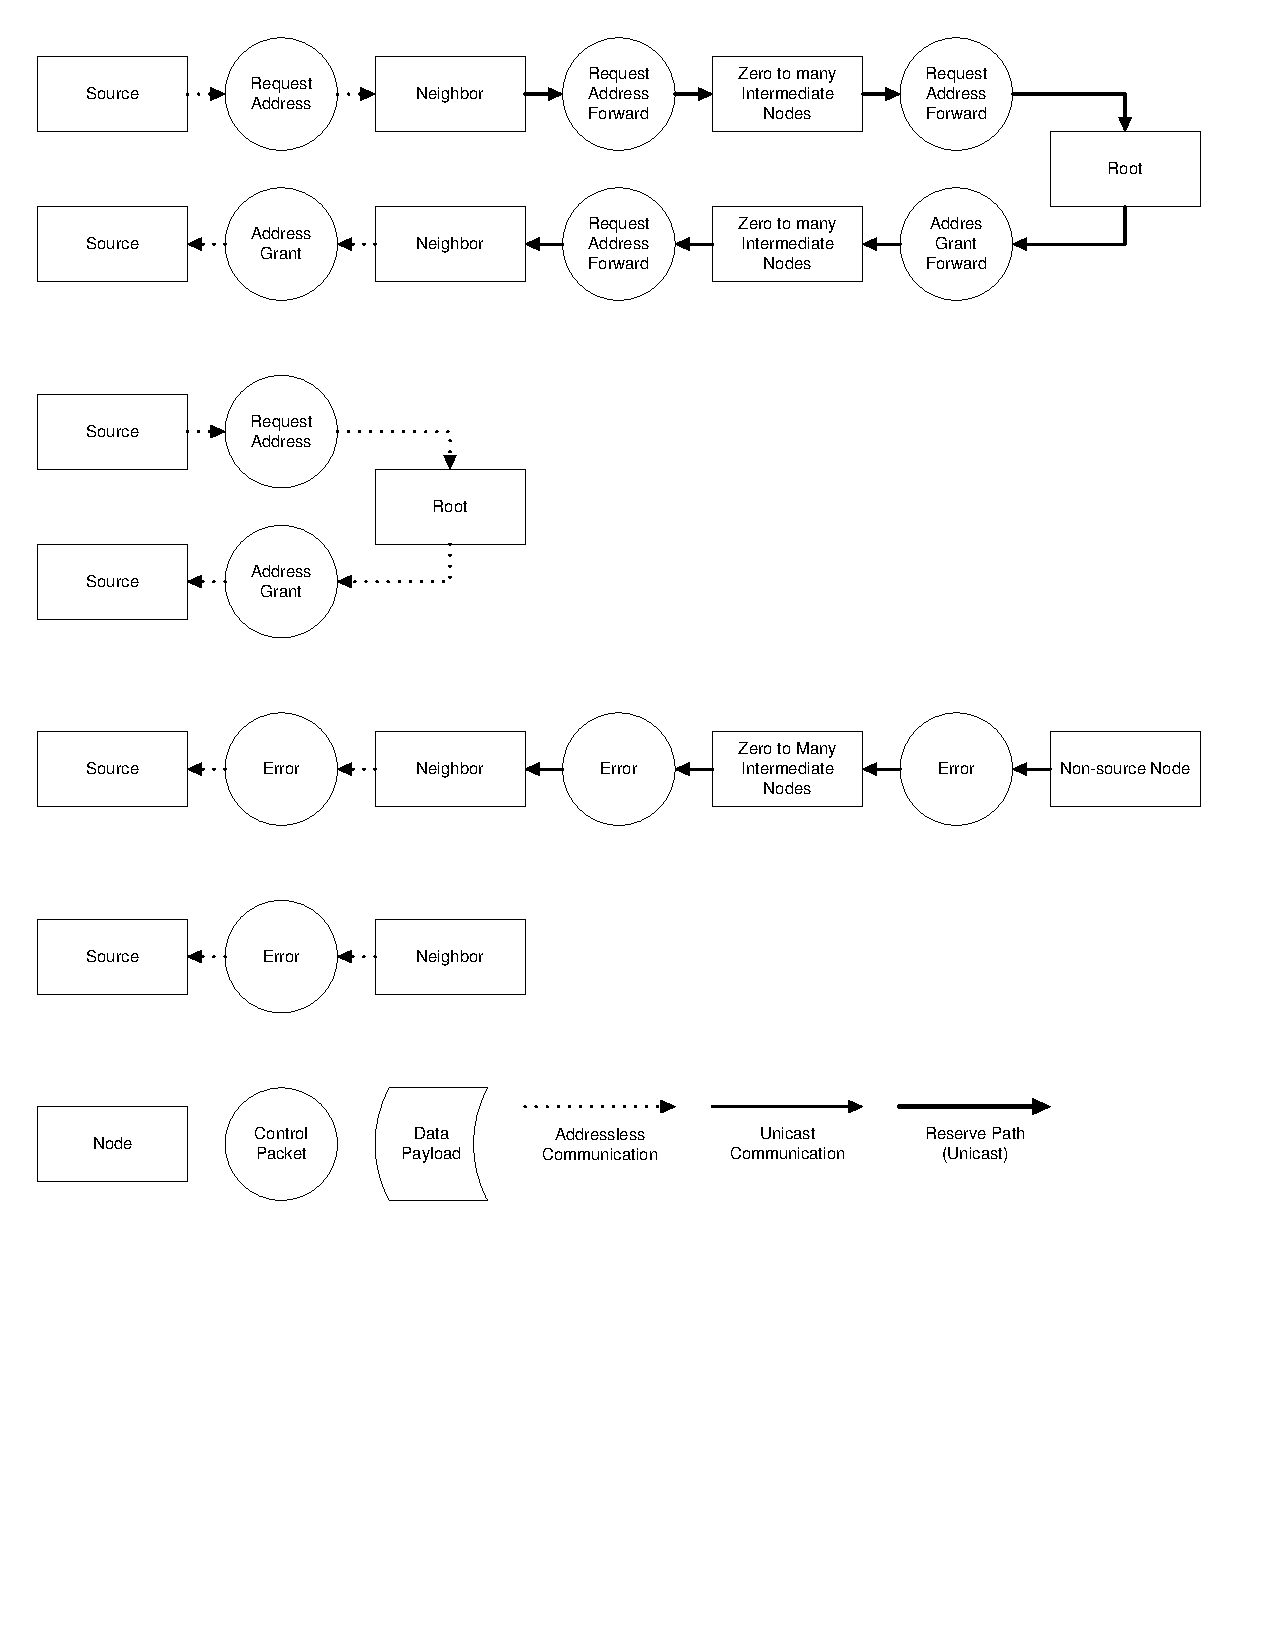
\includegraphics[scale=0.75]{Protocol/Figures/protocol-request_address.pdf}
		\caption{Flow diagram for the Request Address Command}
		\label{fig:protocol:request_address}
	\end{centering}
\end{figure}

\subsubsection{Report Neighbors}\label{ref:protocol:methodology:commands:report_neighbors}

After a node has gained an address, it sends a list of its neighbors to the root so that the root can generate the routing table. A node is ready to report its neighbors after a) it has received an address and b) all of its neighbors have received an address. Each node sends the address of its neighbors and the link to which they are connected. This information can be encoded into the command specific fields of a control packet, because each F2808 has four links, thus eliminating the need to do a full data transfer. The list of sequence steps are shown in Table \ref{tab:protocol:report_neighbors}, and the flow diagram is shown in Figure \ref{fig:protocol:report_neighbors}.

\begin{table}
	\begin{center}
		\setlength{\extrarowheight}{1.5pt}
		\caption{Sequence Steps for the Report Neighbors Command}
		\vspace{0.1cm}
		\begin{tabular}{|l|l|}
			\hline
			\textbf{Sequence Step} & \textbf{Description} \\
			\hline
			\hline
			Report Neighbors & Report neighbor information to the root node \\
			\hline
			Neighbors Received & Acknowledge that the neighbor info was received \\
			\hline
			Error & The request could not be completed \\
			\hline
		\end{tabular}
		\label{tab:protocol:report_neighbors}
	\end{center}
\end{table}

\begin{figure}[ptb]
	\begin{centering}
		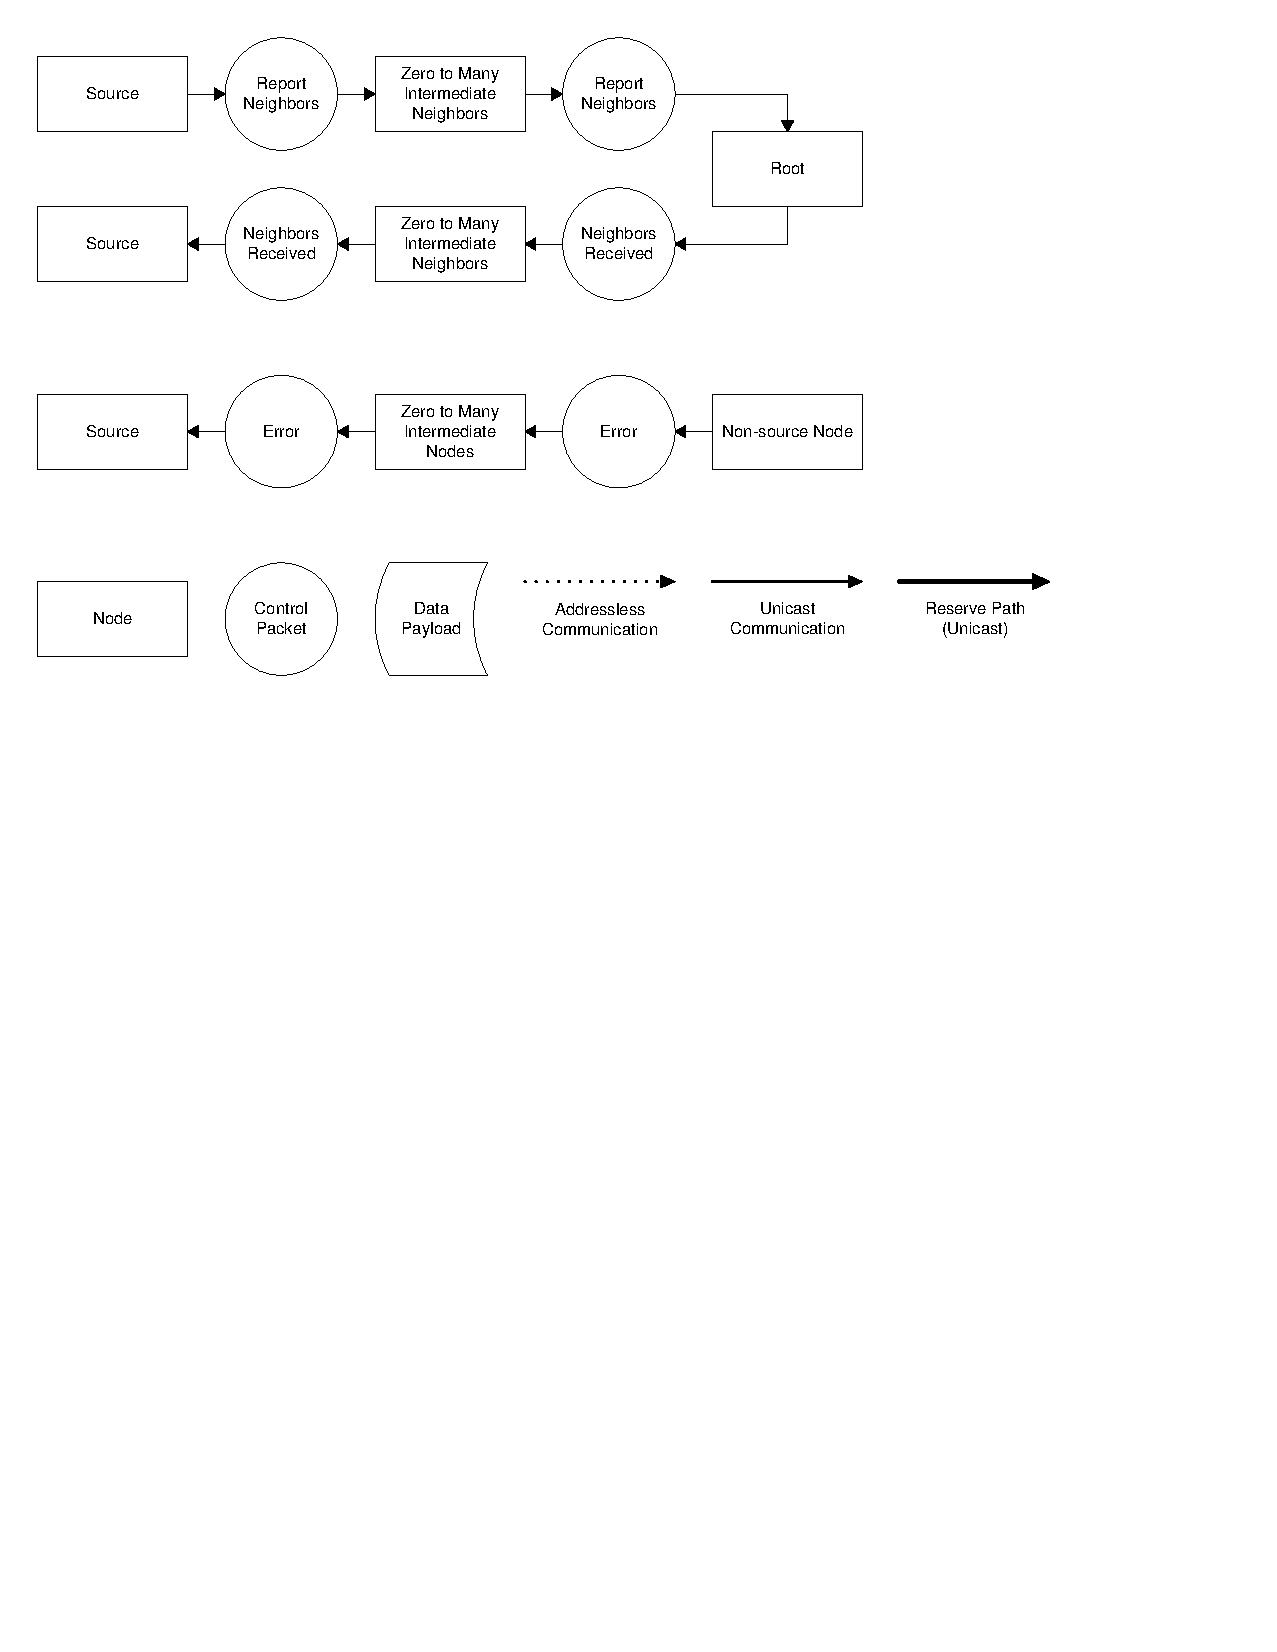
\includegraphics[scale=0.75]{Protocol/Figures/protocol-report_neighbors.pdf}
		\caption{Flow diagram for the Report Neighbors Command}
		\label{fig:protocol:report_neighbors}
	\end{centering}
\end{figure}

\subsubsection{Routing Table Available}\label{ref:protocol:methodology:commands:routing_table_available}

When the root node has received the neighbor information from all nodes that have requested an address, the root node can then generate the routing table. A new routing table is also generated when a communication failure is detected. After the table has been generated, the root node informs all of the other nodes that the routing table is available via the Routing Table Available command. Note that an ACK sequence step is not used for this command because this command is always followed by the Request Routing Table command, which inherently acts as an ACK. The list of sequence steps are shown in Table \ref{tab:protocol:routing_table_available}, and the flow diagram is shown in Figure \ref{fig:protocol:routing_table_available}.

\begin{table}
	\begin{center}
		\setlength{\extrarowheight}{1.5pt}
		\caption{Sequence Steps for the Routing Table Available}
		\vspace{0.1cm}
		\begin{tabular}{|l|l|}
			\hline
			\textbf{Sequence Step} & \textbf{Description} \\
			\hline
			\hline
			Routing Table Available & Informs that a new routing table is available \\
			\hline
			Error & The request could not be completed \\
			\hline
		\end{tabular}
		\label{tab:protocol:routing_table_available}
	\end{center}
\end{table}

\begin{figure}[ptb]
	\begin{centering}
		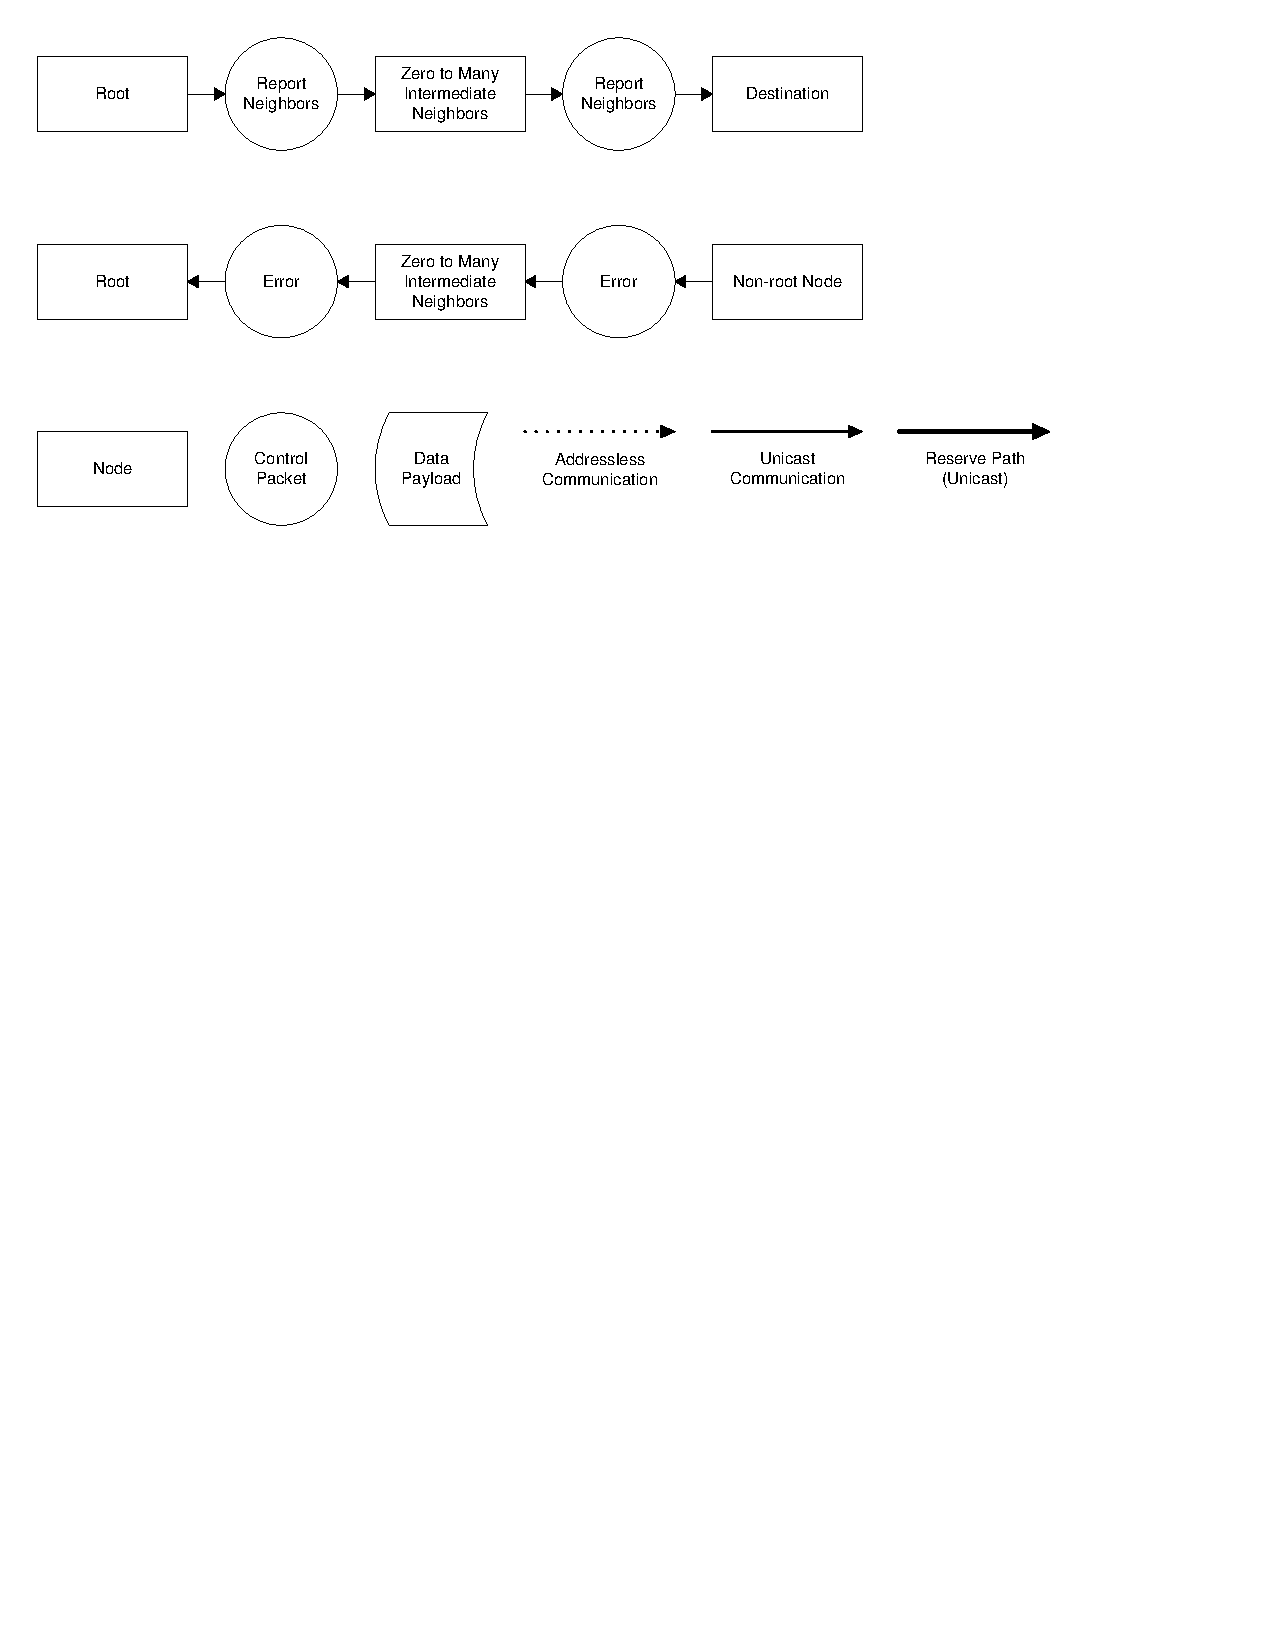
\includegraphics[scale=0.75]{Protocol/Figures/protocol-routing_table_available.pdf}
		\caption{Flow diagram for the Routing Table Available Command}
		\label{fig:protocol:routing_table_available}
	\end{centering}
\end{figure}

\subsubsection{Request Routing Table}\label{ref:protocol:methodology:commands:request_routing_table}

When a new node receives the New Routing Table Available command, it then requests a new copy of the routing table using the Request New Routing Table command. The node starts by requesting the routing table from the root node. In response, the root sends a request to perform a data transfer and sends the 32-bit CRC of the data and the data length in the command specific fields. This request primarily reserves the path from the root to the node. When the node has received the request, it lets the root node know that it got the request, which implies that the path has also been reserved. When the root receives confirmation of path reservation, it sends the data payload. When the node has received all of the data, the node checks the data for errors and then replies that it correctly received the data. Note that the reserved paths are released after the last flit in the data payload is sent through. The list of sequence steps are shown in Table \ref{tab:protocol:request_routing_table}, and the flow diagram is shown in Figure \ref{fig:protocol:request_routing_table}.

\begin{table}
	\begin{center}
		\setlength{\extrarowheight}{1.5pt}
		\caption{Sequence Steps for the Request Routing Table Command}
		\vspace{0.1cm}
		\begin{tabular}{|l|l|}
			\hline
			\textbf{Sequence Step} & \textbf{Description} \\
			\hline
			\hline
			Request Routing Table & Request the routing table from the root node \\
			\hline
			Request Table Transfer & Reserves the path between the root and the node \\
			\hline
			Transfer Request Accepted & Indicates the path reservation is complete \\
			\hline
			Table Transfer & Transfers the data flit by flit to the node \\
			\hline
			Transfer Completed Successfully & The transfer was completed successfully \\
			\hline
			Error & The request could not be completed \\
			\hline
		\end{tabular}
		\label{tab:protocol:request_routing_table}
	\end{center}
\end{table}

\begin{figure}[ptb]
	\begin{centering}
		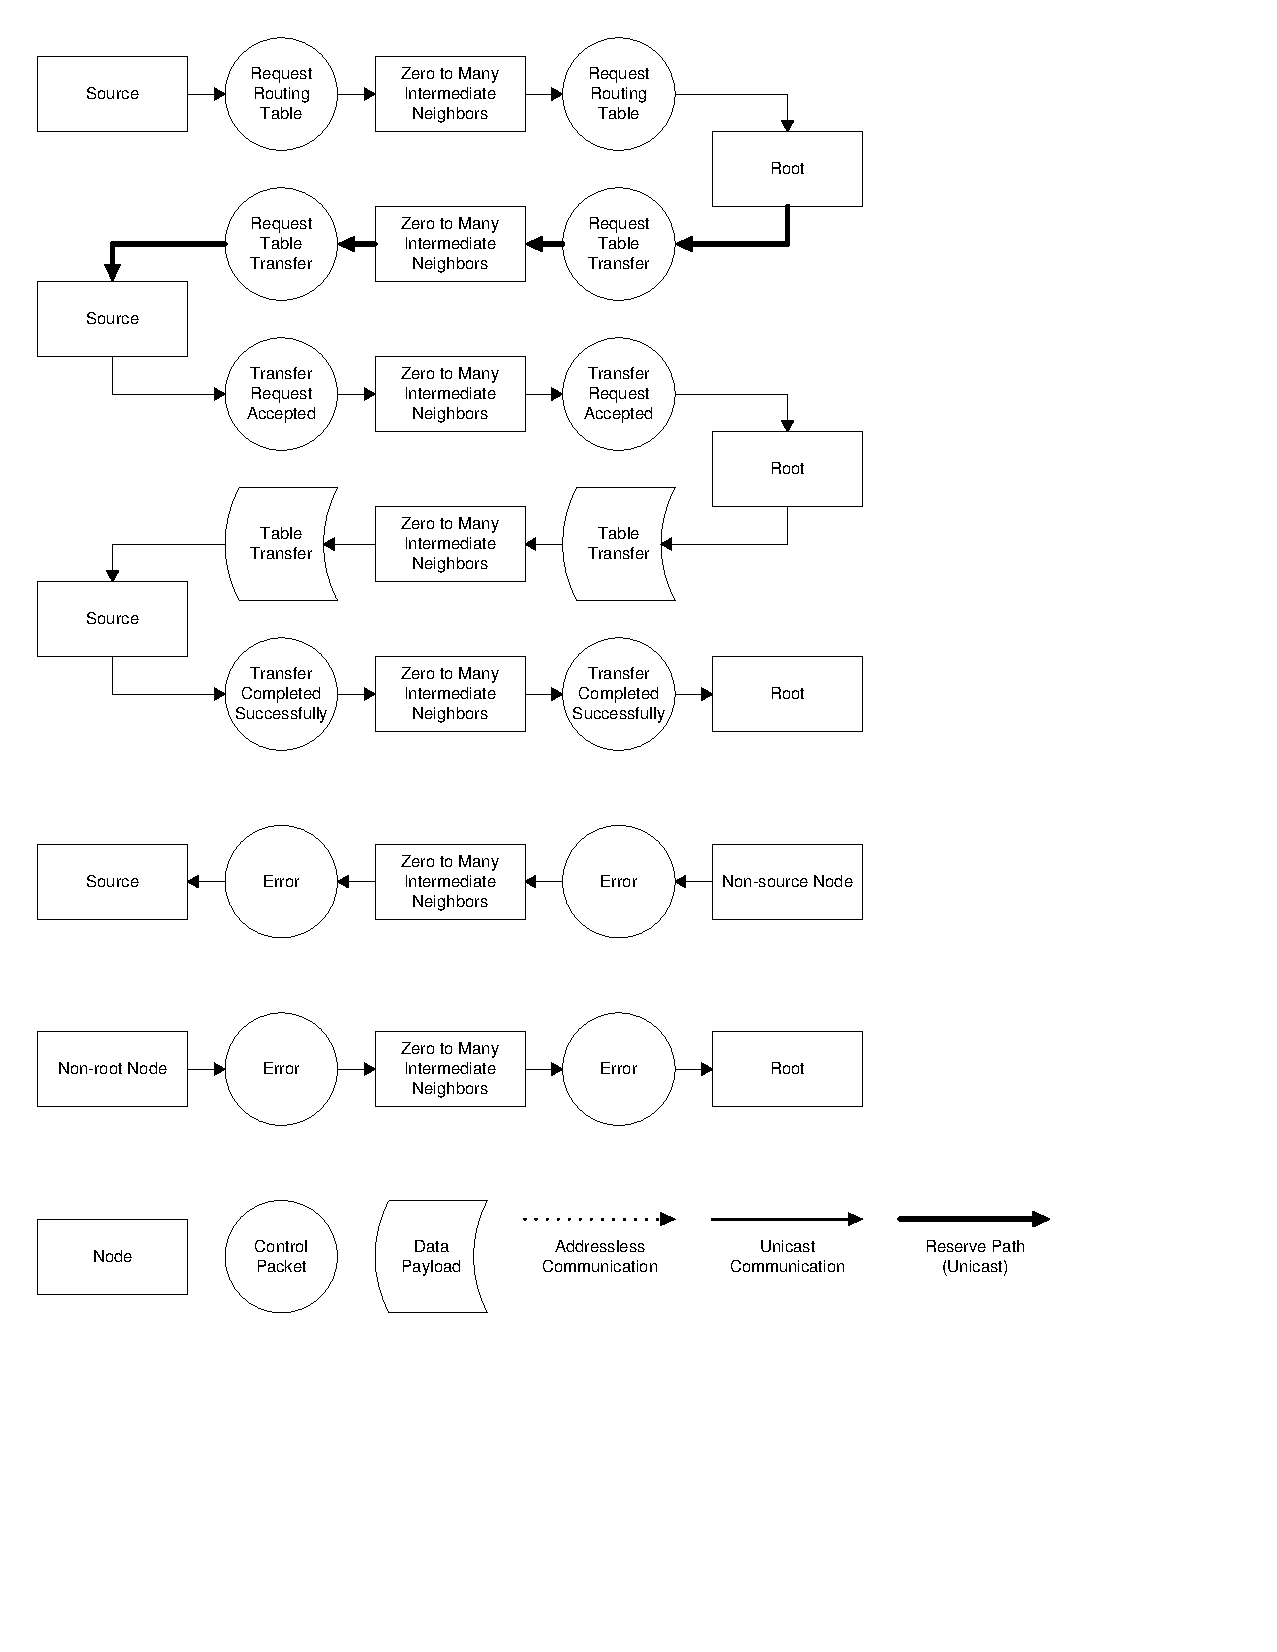
\includegraphics[scale=0.75]{Protocol/Figures/protocol-request_routing_table.pdf}
		\caption{Flow diagram for the Request Routing Table Command}
		\label{fig:protocol:request_routing_table}
	\end{centering}
\end{figure}
 
\subsubsection{Communication Failure}\label{ref:protocol:methodology:commands:comm_failure}

A node determines that a neighbor has disappeared when it doesn't respond to a preset number of Discover Neighbor commands, after having previously responded to said commands at some point in time. In this scenario, the node that discovered the missing neighbor sends a Communication Failure command to the root, which causes the root to regenerate the routing table. The list of sequence steps are shown in Table \ref{tab:protocol:comm_failure} and the flow diagram is shown in Figure \ref{fig:protocol:comm_failure}.

\begin{table}
	\begin{center}
		\setlength{\extrarowheight}{1.5pt}
		\caption{Sequence Steps for the Communication Failure Command}
		\vspace{0.1cm}
		\begin{tabular} {|l|l|}
			\hline
			\textbf{Sequence Step} & \textbf{Description} \\
			\hline
			\hline
			Communication Failure & Reports which node stopped communication to the root \\
			\hline
			Error & The request could not be completed \\
			\hline
		\end{tabular}
		\label{tab:protocol:comm_failure}
	\end{center}
\end{table}

\begin{figure}[ptb]
	\begin{centering}
		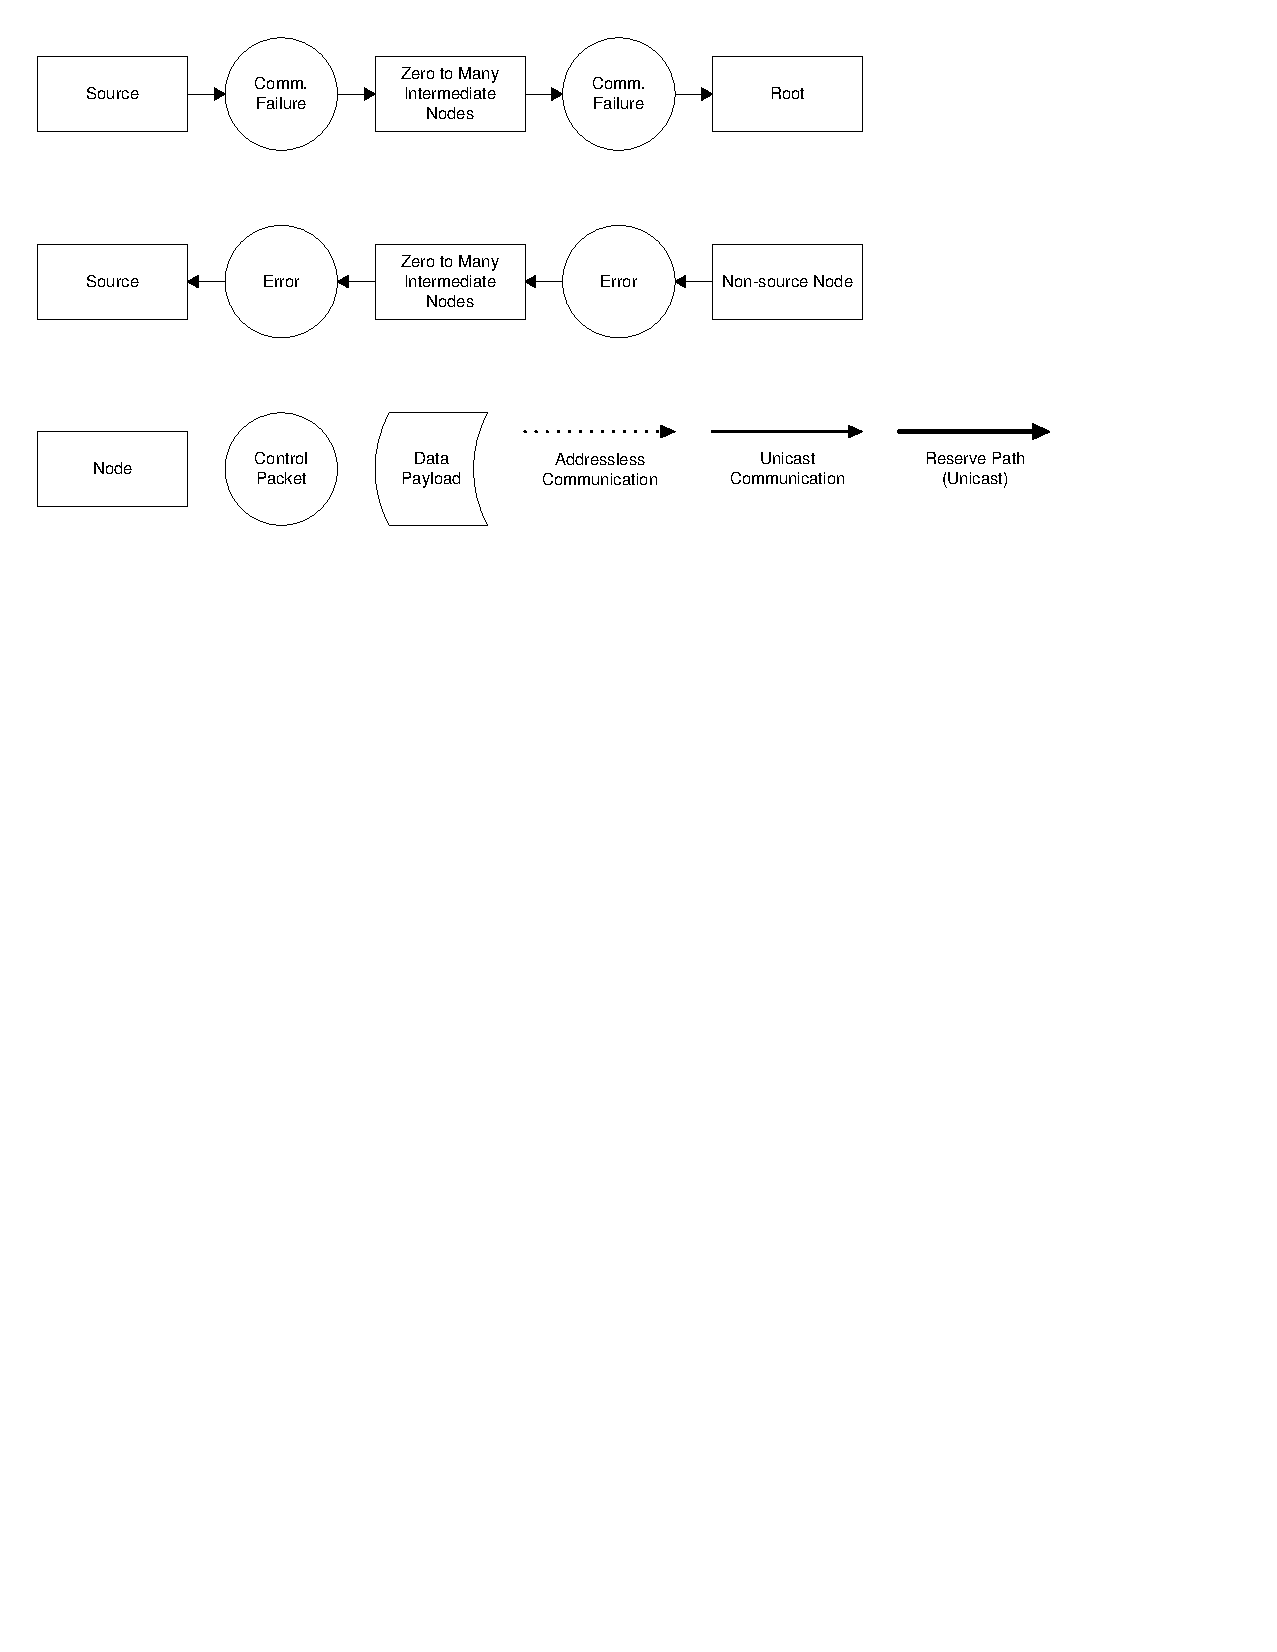
\includegraphics[scale=0.75]{Protocol/Figures/protocol-comm_failure.pdf}
		\caption{Flow diagram for the Communication Failure Command}
		\label{fig:protocol:comm_failure}
	\end{centering}
\end{figure}

\subsubsection{Data Transfer}\label{ref:protocol:methodology:commands:data_transfer}

Data transfers are basically identical to the request routing table command, except that the initial request sequence step is not used and the destination can be any other node. The list of sequence steps are shown in Table \ref{tab:protocol:data_transfer}, and the flow diagram is shown in Figure \ref{fig:protocol:data_transfer}.

\begin{table}
	\begin{center}
		\setlength{\extrarowheight}{1.5pt}
		\caption{Sequence Steps for the Data Transfer Command}
		\vspace{0.1cm}
		\begin{tabular} {|l|l|}
			\hline
			\textbf{Sequence Step} & \textbf{Description} \\
			\hline
			\hline
			Request Data Transfer & Reserves a path from the source to destination \\
			\hline
			Transfer Request Accepted & Indicates the path reservation is complete \\
			\hline
			Data Transfer & Transfers the data flit by flit to the destination \\
			\hline
			Transfer Completed Successfully & The transfer was completed successfully \\
			\hline
			Error & The request could not be completed \\
			\hline
		\end{tabular}
		\label{tab:protocol:data_transfer}
	\end{center}
\end{table}

\begin{figure}[ptb]
	\begin{centering}
		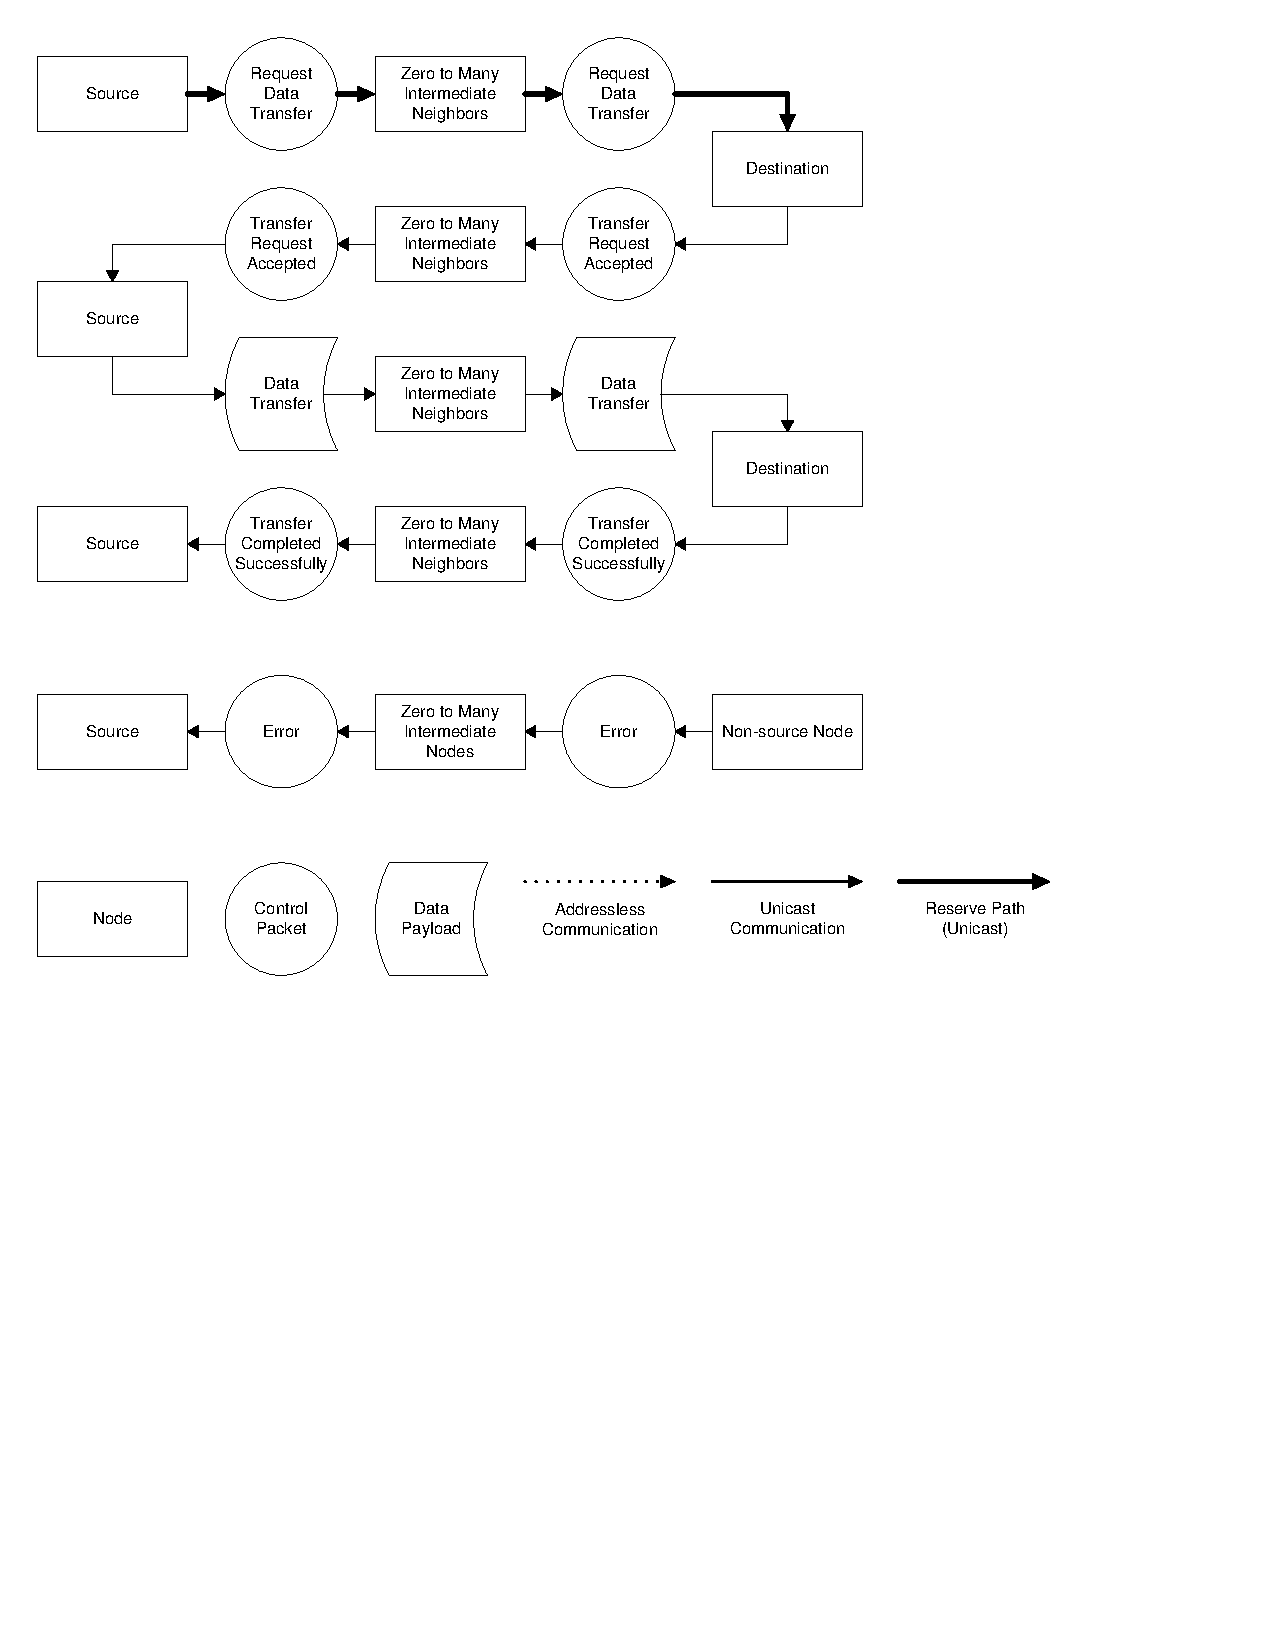
\includegraphics[scale=0.75]{Protocol/Figures/protocol-data_transfer.pdf}
		\caption{Flow diagram for the Data Transfer Command}
		\label{fig:protocol:data_transfer}
	\end{centering}
\end{figure}

\subsubsection{Application Control}\label{ref:protocol:methodology:commands:app_control}

Sometimes an application must send a packet that does not require a full data transfer. Sometimes the mere fact that a certain type of packet is received is enough information for the application. The Application Control command was created to serve this need. The command specific fields are used to identify the type of application control packet and to store extra parameters. The list of sequence steps are shown in Table \ref{tab:protocol:application_control}, and the flow diagram is shown in Figure \ref{fig:protocol:application_control}.

\begin{table}
	\begin{center}
		\setlength{\extrarowheight}{1.5pt}
		\caption{Sequence Steps for the Application Control Command}
		\vspace{0.1cm}
		\begin{tabular} {|l|l|}
			\hline
			\textbf{Sequence Step} & \textbf{Description} \\
			\hline
			\hline
			Application Control & Sends the control packet \\
			\hline
			Application Control Received & The packet was received successfully \\
			\hline
		\end{tabular}
		\label{tab:protocol:application_control}
	\end{center}
\end{table}

\begin{figure}[ptb]
	\begin{centering}
		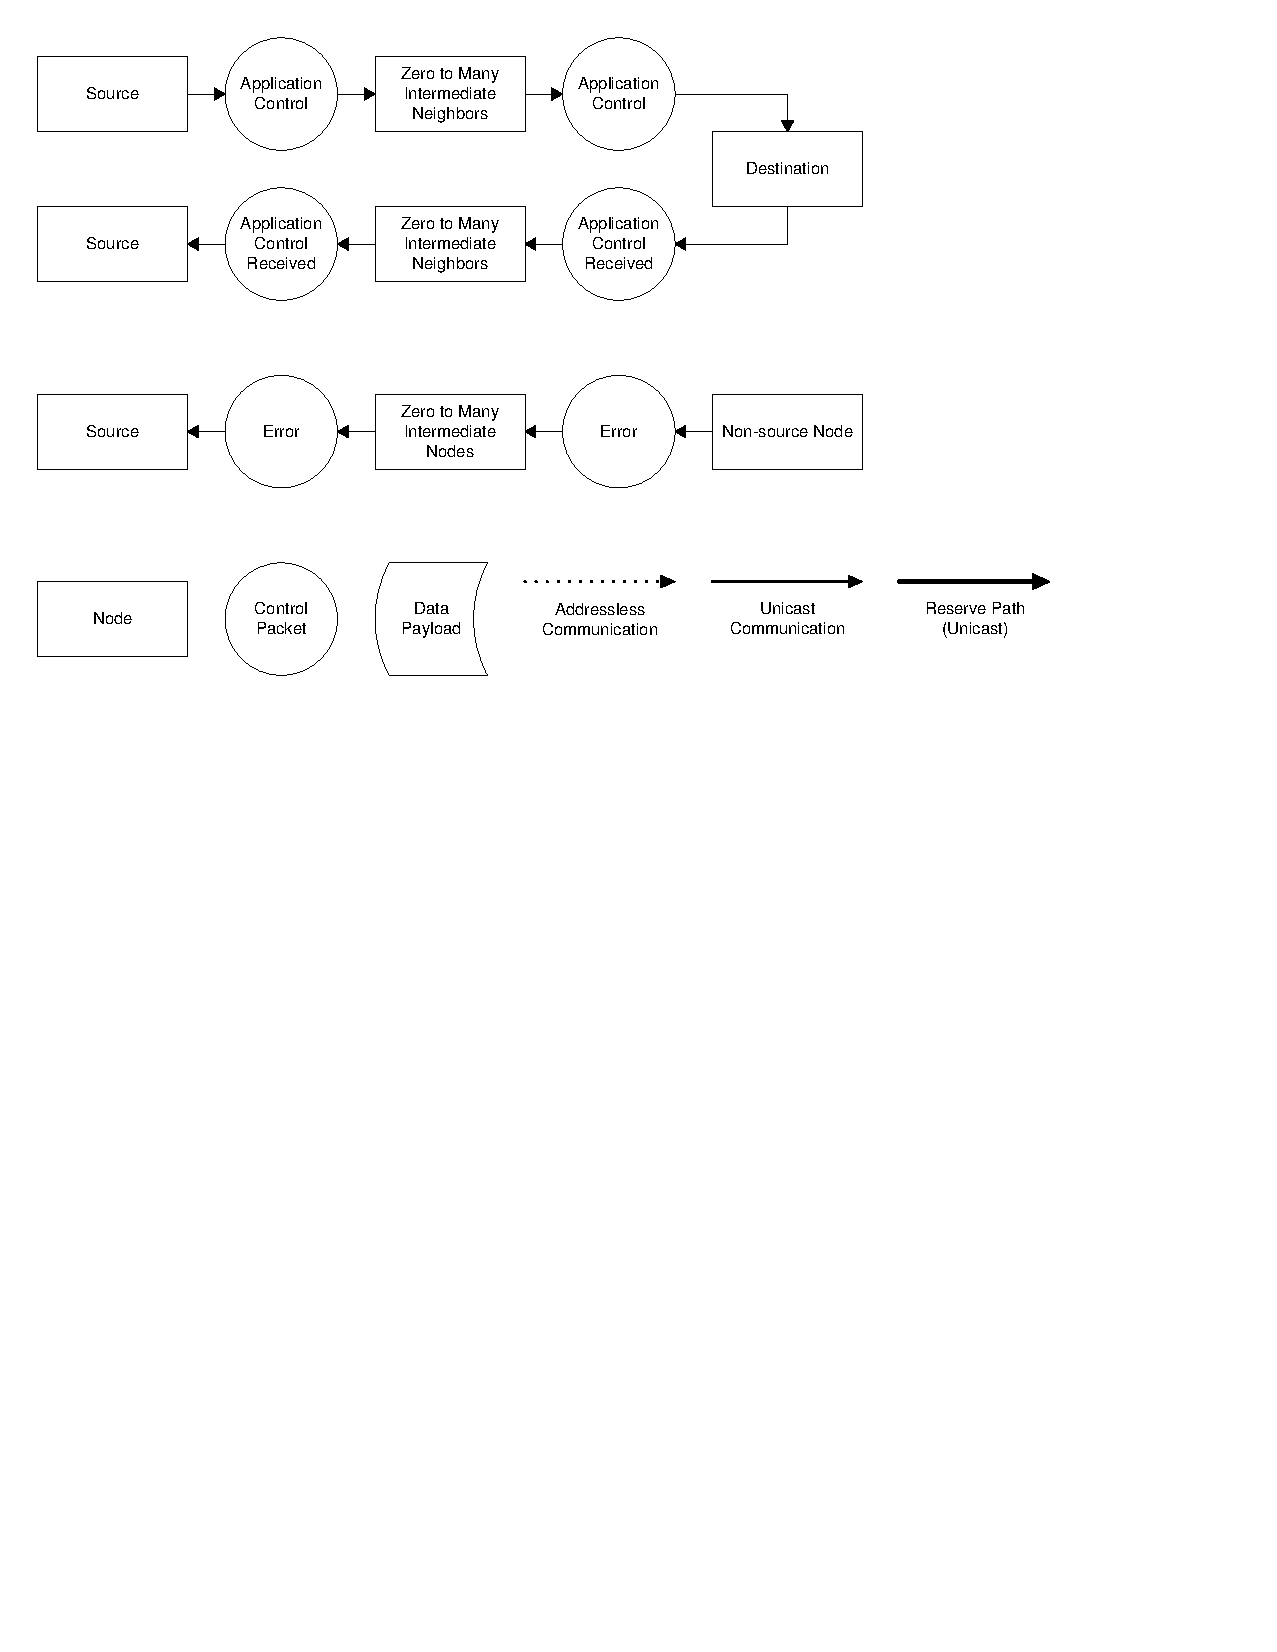
\includegraphics[scale=0.75]{Protocol/Figures/protocol-application_control.pdf}
		\caption{Flow diagram for the Application Control Command}
		\label{fig:protocol:application_control}
	\end{centering}
\end{figure}

\section{Implementation}\label{sec:protocol:implementation}

The code that implements the protocol is divided into three categories: packet handling functions, the protocol stack, and data transfer handling.

\subsection{Packet Handling Functions}\label{sec:protocol:implementation:packet_handling}

The packet handling functions are a set of helper functions for working with packets. These functions include various means of initializing packets, marshaling and unmarshaling packets, copying packets, etc.

Three ways are available to initialize a packet: default initialization, initializing a packet using the packet from the previous command sequence step, and re-initializing a packet that has already been initialized. The default initialization function sets as much of the packet as it can without knowing how the packet will be used (e.g. the source is set, but the destination is not). When a packet is initialized from the previous sequence step, it takes advantage of the fact that whenever a packet is processed, it always corresponds to a specific sequence step. Because the next sequence step uses a packet that is almost identical, most of the information from the previous packet is re-used. On occasion, it is necessary to process a packet and forward it to another router, such as when reserving the path for a data transfer. In this case, the initialize-from-self function does not modify the information contained in the header, but does reset non-packet-header information, such as the virtual channel used to transmit on.

Four functions for marshaling and unmarshaling packet headers and data are available. The header marshaling and unmarshaling functions stuff the \lstinline$struct$ organized fields of the header into a numerical array and back again, with each array element containing 16 bits of the header. Header marshaling/unmarshaling also calculates the CRC8 using the 0x07 polynomial and determines whether a CRC8 has failed. Data marshaling is performed a little differently: only one flit is marshaled at a time. In order to increase memory efficiency, data is marshaled and unmarshaled \emph{on demand}, i.e. the next flit is not marshaled until it is needed for transmission, thus eliminating the need to store marshaled flits at the source node. Data unmarshaling is performed in a similar manner; a flit is unmarshaled as soon as it arrives, which eliminates the need to buffer marshaled data at the destination node. CRC32 checking using the 0x04C11DB7 polynomial is done before marshaling has begun and after unmarshaling is complete.

\subsection{Protocol Stack Functions}\label{sec:protocol:implementation:protocol_stack}

The protocol stack consists of a series of nested \lstinline$switch$ statements that first check the command and then the packet sequence step. This code basically follows the flow diagrams shown in Section \ref{sec:protocol:methodology:commands}. A series of \emph{protocol actions} that initiate commands are available because the protocol stack only responds to \emph{received} packets by definition, and so some action is needed to initiate the process. There are five protocol actions: neighbor follow-up, report neighbors, request routing table, handle communication error, and ensure routing table distribution. The request routing table protocol action simply sends a request routing table protocol command to the root.

The neighbor follow-up protocol action is responsible for initiating the discover neighbors protocol command. This action is also responsible for determining if a neighbor has stopped communicating. This action runs periodically (currently every 5 seconds), and if a neighbor hasn't responded to a discover neighbors command by the time the action runs again, then it is considered to have not responded to the request. A neighbor is considered to have failed if it does not respond 3 times in a row, whereupon the node sends a communication failure protocol command to the root. Thus, the minimum time between a node failure and the root being informed of that error is 15 seconds given the current configuration.

The report neighbors protocol action is run when the node has acquired an address from the root. If all of the neighbors have reported an acquired address via the discover neighbors command, then this action reports the neighbors to the root, otherwise it schedules itself to run at a later point in time to give the neighbors a chance to acquire an address. 

The handle communication error is called whenever a CRC error in a packet header or data payload is detected. This action creates a packet with the Error sequence step, which is (not coincidentally) the same enumerated value across all commands, and sends it back to the node that sent the flit. Sometimes the source node is unknown, as in the case when a packet header fails its CRC check and the header was not sent using addressless communication. When this happens, the action just doesn't do anything.

The ensure routing table distribution protocol action is specifically for the root node. When the new routing table available protocol command is sent out, this action runs periodically until all nodes have successfully received the routing table. When the action runs, it resends the new routing table available command to all nodes that have not successfully received the routing table yet.

\subsection{Data Transfer Handling}\label{sec:protocol:implementation:data_transfers}

Data transfers are composed of three parts: sending data from the source, forwarding data through an intermediate node, and buffering data at the destination. 

Sending data first involves sending a probe message, so the data payload is stored temporarily until the acknowledgement is received. A timeout is implemented in case the probe gets lost. The probe is sent out on the virtual channel that is to be used for the data transfer, so that the next node in the path can link an incoming port/virtual channel pair to a destination. When the acknowledgement has been received, the source begins to marshal the data one flit at a time and sends the marshaled flit on the reserved virtual channel.

Data forwarding occurs when a node in the path is not the destination or the source. The probe packet is processed by the protocol stack so that a virtual channel can be reserved on the appropriate output path, and a link between the input port/virtual channel pair and the output port/virtual channel pair is established. When a data payload end flit type is received on the appropriate input port/virtual channel pair, the reservation is removed.

When a probe packet is received at the destination, a buffer is allocated for the unmarshaled data, and the header is saved for later reference. Buffering is essentially the same as data forwarding, except that a link is established between the input port/virtual channel pair and a buffer, and each flit is immediately unmarshaled when it is received. The CRC32 is calculated when a data payload end flit type is received, and a callback function associated with the appropriate command type is called that finalizes the transfer. This callback sends an acknowledgement packet to the source if the CRC32 check is passed; otherwise an error packet is sent. The error packet is for purely informative purposes; guaranteed delivery is left to higher network layers.

\section{Results}\label{sec:protocol:results}

Two factors of the protocol are considered: reliability and performance. If a system is not reliable, then there is no point in discussing any other topics. If the system does not perform well enough, then no one will want to use the system.

\subsection{Reliability}\label{sec:protocol:results:reliability}

To determine if the protocol is reliable, two tests have been devised that heavily stress the system. The first test has multiple nodes streaming through a bottleneck to a single destination. The other test has a single node streaming to the other nodes through a staggered bottleneck. 

The first test is designed to stress singular bottlenecks by streaming data from the non-root nodes to the root with a bottleneck in between. The nodes are configured in a ``T'' shape with the root at the bottom of the ``T,'' which creates a bottleneck at node 2. The test was first run with node 2 just acting as a router, shown in Figure \ref{fig:protocol:2_t_flood_test}, and then with node 2 also streaming data to the root, as shown in Figure \ref{fig:protocol:3_t_flood_test}. The results for the 2 transmitting nodes test are in Table \ref{tab:protocol:2_t_flood_test}, and show that the system worked flawlessly. The results for the 3 transmitting nodes test are shown in Table \ref{tab:protocol:3_t_flood_test}, and show that the system was almost perfect, but had a few mistakes. The packets that did not complete successfully had timed out. This occurred because node 2 was overworked. Most of the packets that failed originated at node 2, which is expected because the code that initiates transfers runs at a lower priority than the protocol stack, which runs at a lower priority than the SPI code, thus causing starvation of the transfer code. As a result, the code initiating transfers rarely gets a chance to run, and the associated transfers have already timed out when it does finally run. The other packet failures occur because combining three streams into one results in roughly $1/3$ the available bandwidth per stream, and the transmission time begins to approach the timeout limit. When these transfers occur at the exact same time as another (possibly internal) delay, the timeout limit is exceeded. This timing issue could be solved by increasing the timeout, but has the disadvantage of leaving both communication and memory resources tied up, which can lead to the system not being able to fulfill other requests. This scenario is infrequent enough that it is of little concern. This test also shows that the error detection and recovery code works properly, because the system would have run out of resources that should have been released without it.

\begin{figure}[ptb]
	\begin{centering}
		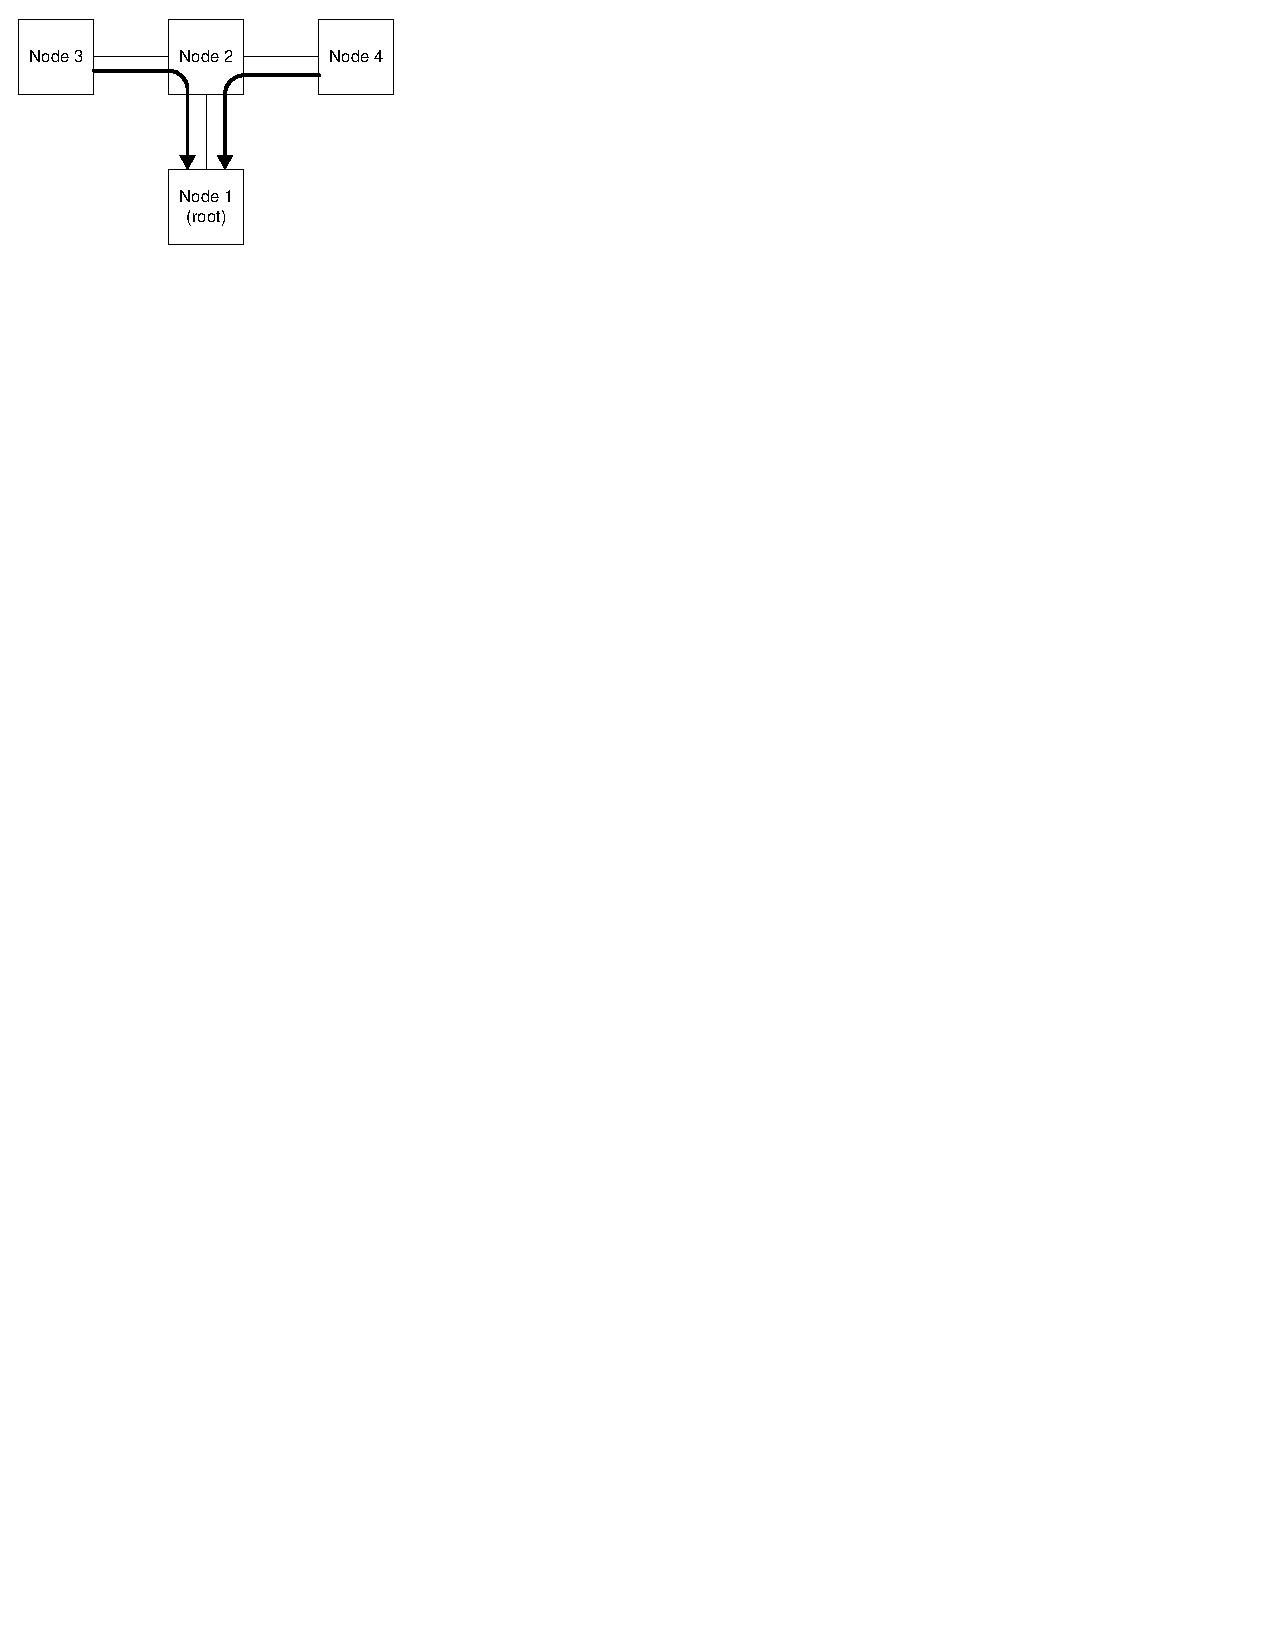
\includegraphics{Protocol/Figures/protocol-2_t_flood_test.pdf}
		\caption{Test setup for single destination test (2 nodes transmitting)}
		\label{fig:protocol:2_t_flood_test}
	\end{centering}
\end{figure}

\begin{table}
	\begin{center}
		\setlength{\extrarowheight}{1.5pt}
		\caption{Results for single destination test (2 nodes transmitting, out of 5000)}
		\vspace{0.1cm}
		\begin{tabular} {|c|c|c|}
			\hline
			\textbf{Trial} & \textbf{Node} 3 & \textbf{Node 4} \\
			\hline
			\hline
			1 & 5000 & 5000 \\
			\hline
			2 & 5000 & 5000 \\
			\hline
			3 & 5000 & 5000 \\
			\hline
			\hline
			Average & 5000 & 5000 \\
			\hline
			Success Rate & 100.00\% & 100.00\% \\
			\hline
		\end{tabular}
		\label{tab:protocol:2_t_flood_test}
	\end{center}
\end{table}

\begin{figure}[ptb]
	\begin{centering}
		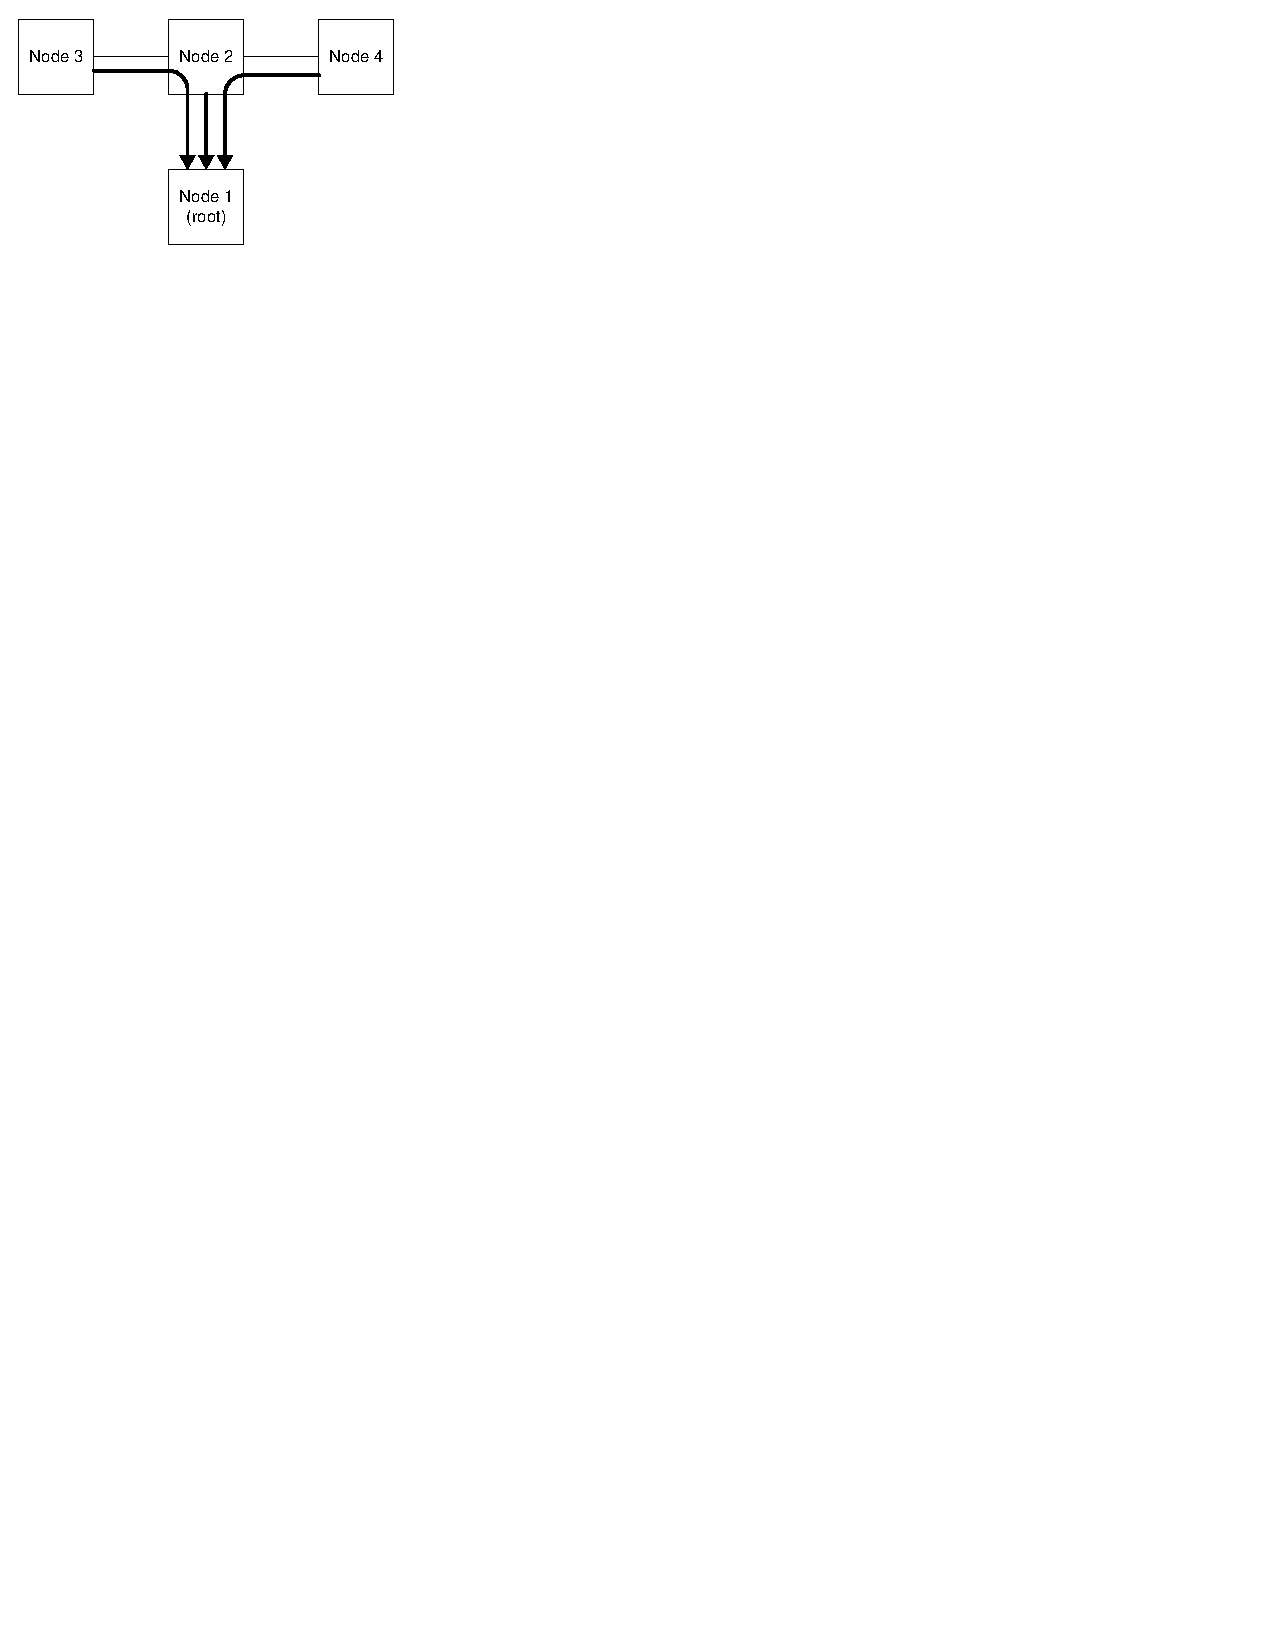
\includegraphics{Protocol/Figures/protocol-3_t_flood_test.pdf}
		\caption{Test setup for single destination test (3 nodes transmitting)}
		\label{fig:protocol:3_t_flood_test}
	\end{centering}
\end{figure}

\begin{table}
	\begin{center}
		\setlength{\extrarowheight}{1.5pt}
		\caption{Results for single destination test (3 nodes transmitting, out of 5000)}
		\vspace{0.1cm}
		\begin{tabular} {|c|c|c|c|}
			\hline
			\textbf{Trial} & \textbf{Node 3} & \textbf{Node 2} & \textbf{Node 4} \\
			\hline
			\hline
			1 & 5000 & 4987 & 4997 \\
			\hline
			2 & 4998 & 4987 & 5000 \\
			\hline
			3 & 4999 & 4986 & 4998 \\
			\hline
			\hline
			Average & 4999.00 & 4986.67 & 4998.33 \\
			\hline
			Success Rate & 99.98\% &99.73\% &99.97\% \\
			\hline
		\end{tabular}
		\label{tab:protocol:3_t_flood_test}
	\end{center}
\end{table}

The next test is designed to stress distributed bottlenecks. The nodes are configured in a straight line, and one node simultaneously and continuously transmits to the other nodes along the line. This has the effect of placing all of the nodes under stress, with the closest node under the most stress. The test was run twice, with the first instance having the root transmitting to the two furthest nodes, as shown in Figure \ref{fig:protocol:2_line_flood_test}, and the second instance with the root transmitting to all three nodes, as shown in Figure \ref{fig:protocol:3_line_flood_test}. The results were reminiscent of the first test, with the 2 destination test working flawlessly, as shown in Table \ref{tab:protocol:2_line_flood_test}, and the 3 destination test having a few problems, as shown in Table \ref{tab:protocol:3_line_flood_test}. In this case, the problems were the same as nodes 3 and 4 had in the first test, where node 2 became overworked and caused timeouts to start occurring. One key difference between this test and the previous is that node 2 did not have nearly as many errors. This difference has to do with the difference in code priority between transmitting and receiving. Receiving is intentionally designed to have a higher priority than transmitting as a flow control mechanism, and the results here are evident.

\begin{figure}[ptb]
	\begin{centering}
		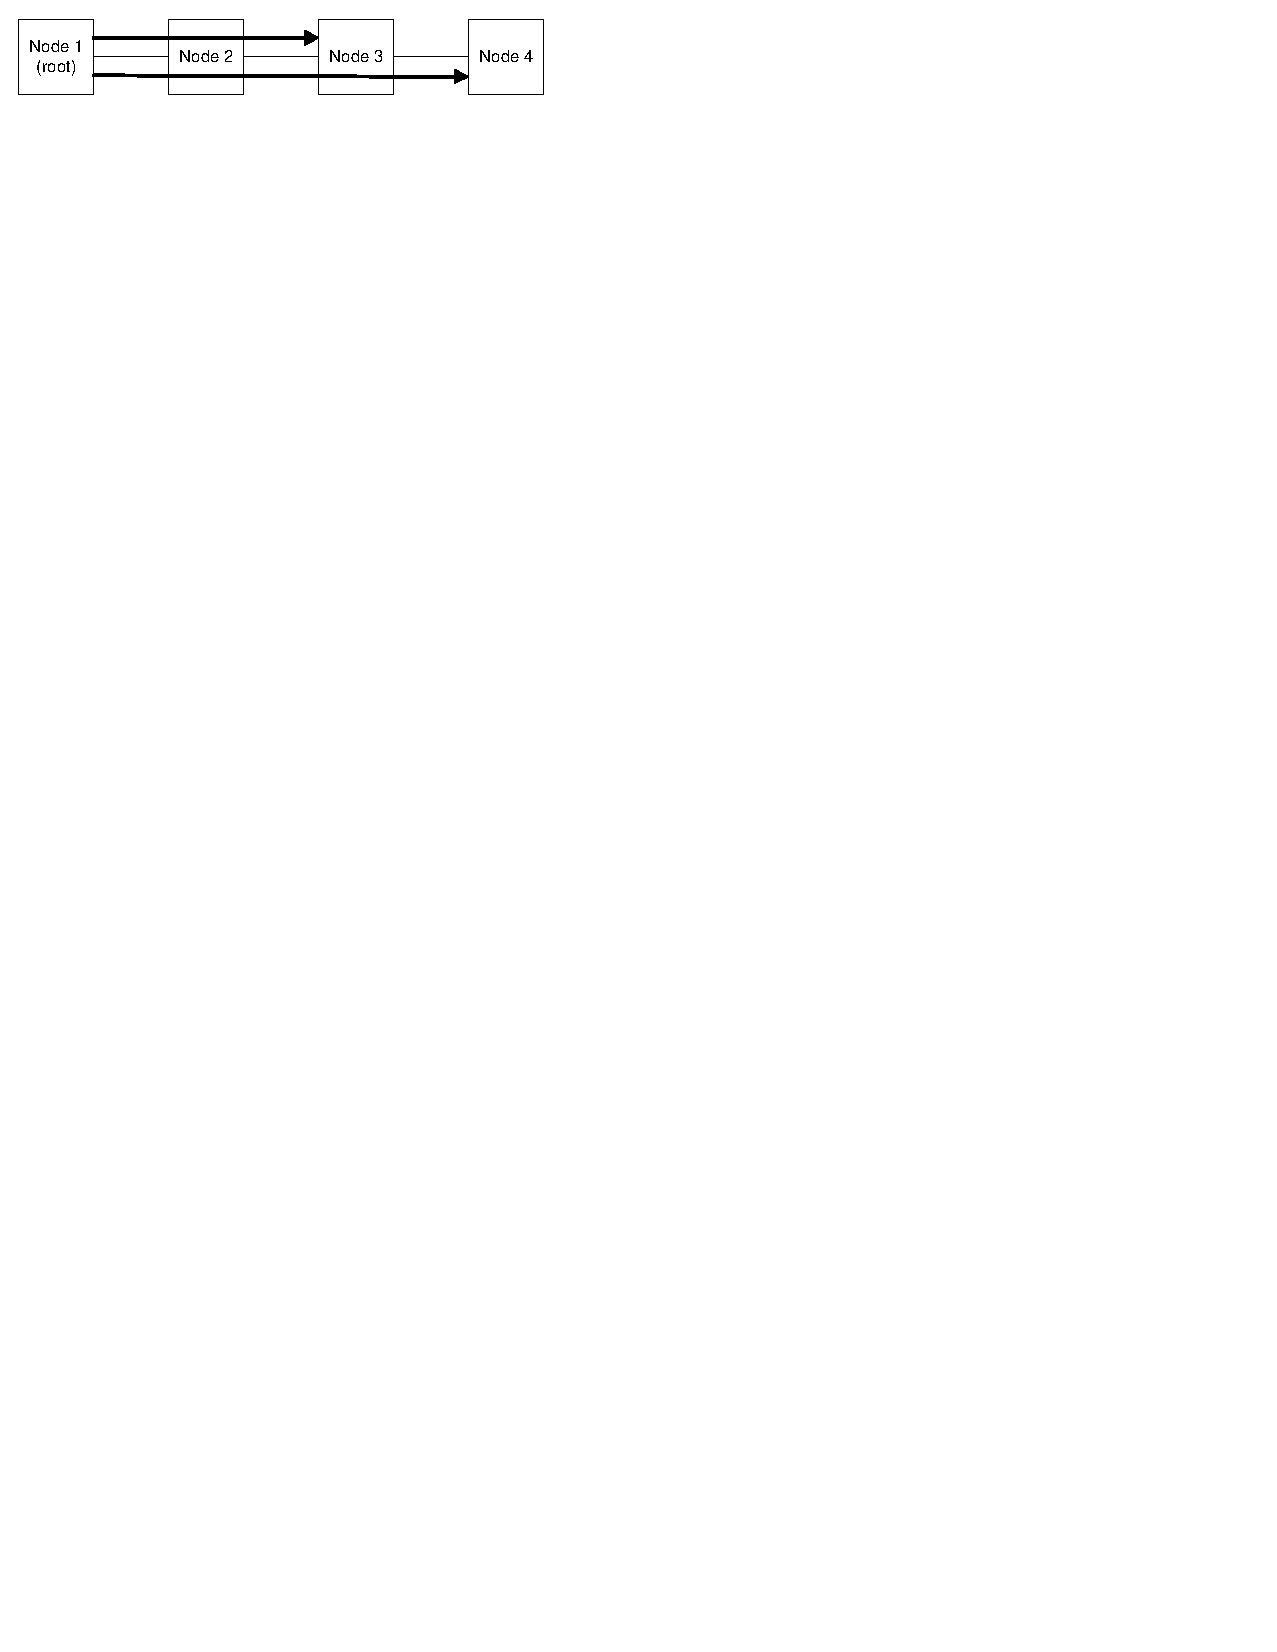
\includegraphics{Protocol/Figures/protocol-2_line_flood_test.pdf}
		\caption{Test setup for single source test (2 nodes receiving)}
		\label{fig:protocol:2_line_flood_test}
	\end{centering}
\end{figure}

\begin{table}
	\begin{center}
		\setlength{\extrarowheight}{1.5pt}
		\caption{Results for single source test (2 nodes receiving, out of 4000)}
		\vspace{0.1cm}
		\begin{tabular} {|c|c|}
			\hline
			\textbf{Trial} & \textbf{Successes} \\
			\hline
			\hline
			1 & 4000 \\
			\hline
			2 & 4000 \\
			\hline
			3 & 4000 \\
			\hline
			\hline
			Average & 4000 \\
			\hline
			Success Rate & 100.00\% \\
			\hline
		\end{tabular}
		\label{tab:protocol:2_line_flood_test}
	\end{center}
\end{table}

 \begin{figure}[ptb]
	\begin{centering}
		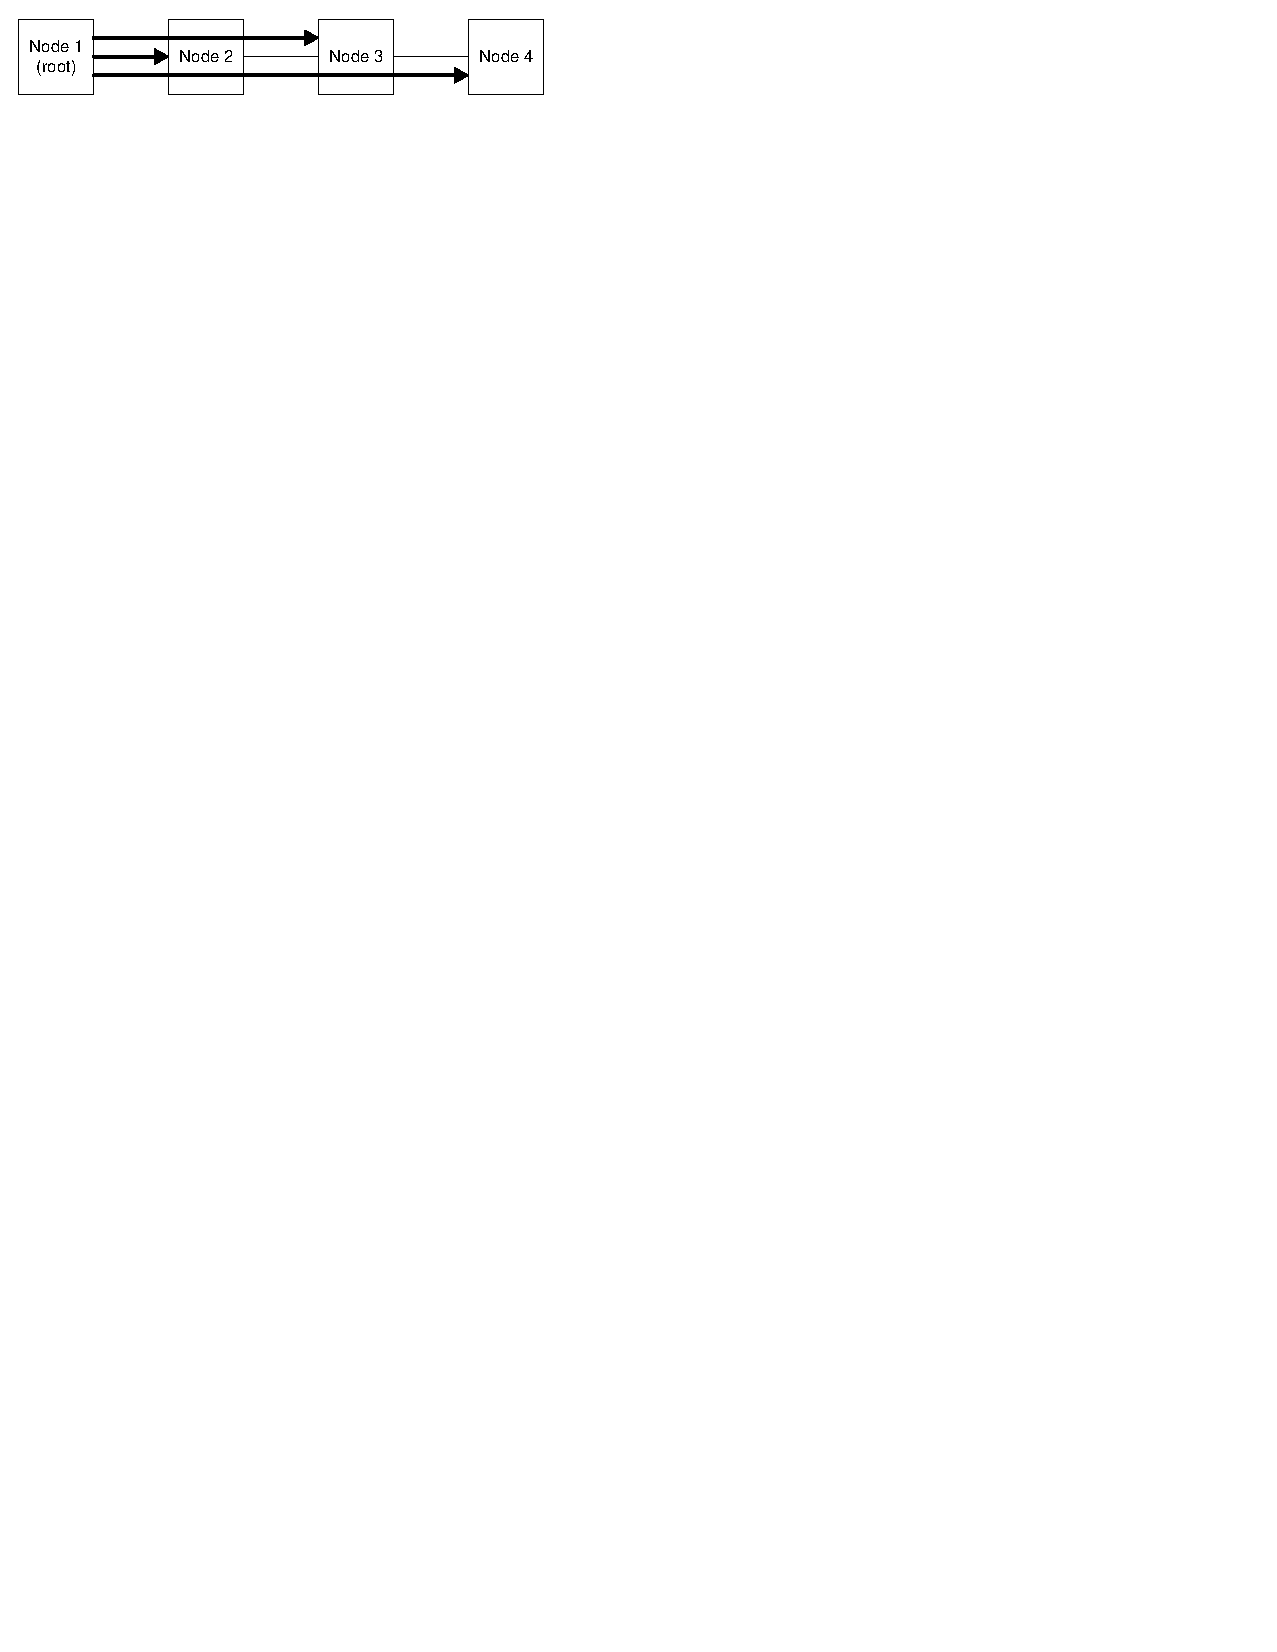
\includegraphics{Protocol/Figures/protocol-3_line_flood_test.pdf}
		\caption{Test setup for single source test (3 nodes receiving)}
		\label{fig:protocol:3_line_flood_test}
	\end{centering}
\end{figure}

\begin{table}
	\begin{center}
		\setlength{\extrarowheight}{1.5pt}
		\caption{Results for single source test (3 nodes receiving, out of 4000)}
		\vspace{0.1cm}
		\begin{tabular} {|c|c|}
			\hline
			\textbf{Trial} & \textbf{Successes} \\
			\hline
			\hline
			1 & 5999 \\
			\hline
			2 & 5999 \\
			\hline
			3 & 6000 \\
			\hline
			\hline
			Average & 5999.33 \\
			\hline
			Success Rate & 99.99\% \\
			\hline
		\end{tabular}
		\label{tab:protocol:3_line_flood_test}
	\end{center}
\end{table}

While not perfect, the system is certainly capable of handling real-world scenarios without issue. These tests also showed, once again, that the timeout detection and recovery mechanisms worked as intended.

\subsection{Performance}\label{sec:protocol:results:performance}

To determine performance, several tests were designed to test latency and throughput. The arrangement of nodes, shown in Figure \ref{fig:protocol:performance_test}, is configured to provide the longest possible path and is used for all of the performance tests.

\begin{figure}[ptb]
	\begin{centering}
		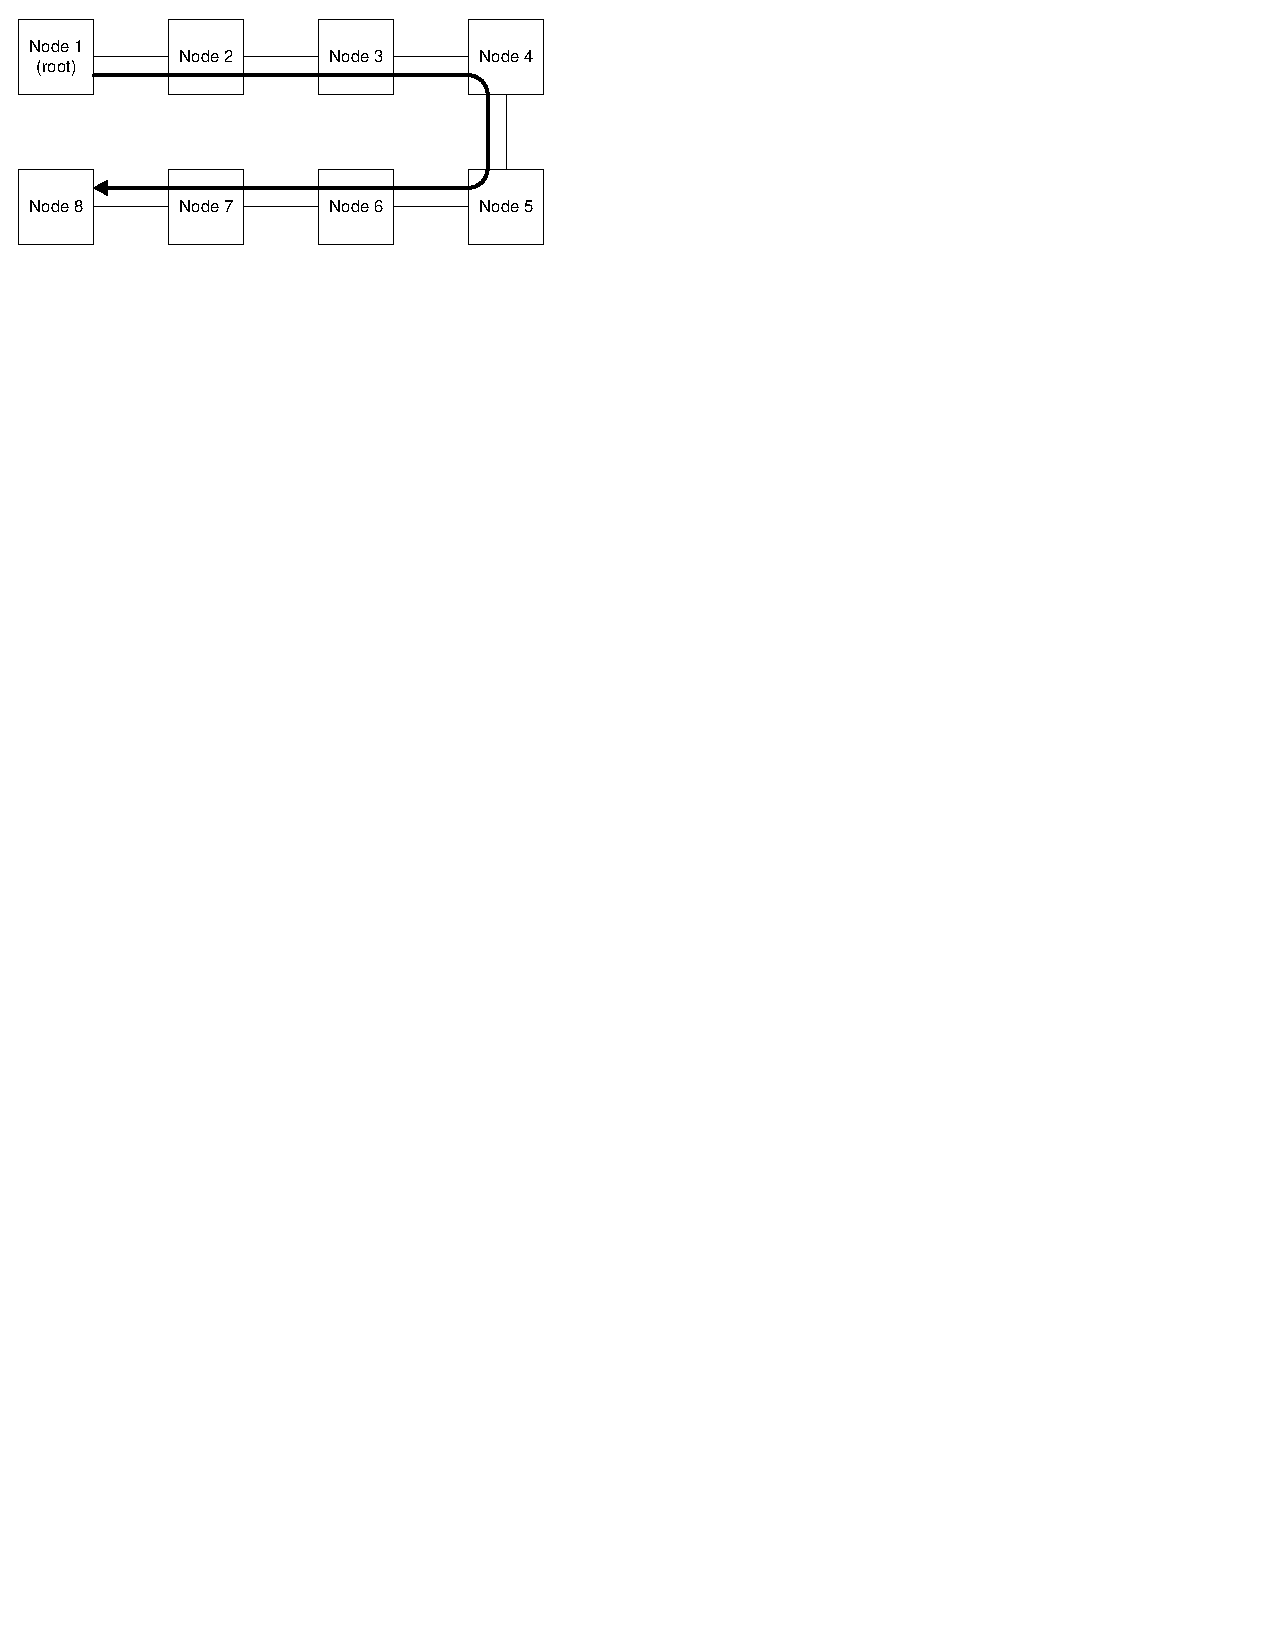
\includegraphics{Protocol/Figures/protocol-performance_test.pdf}
		\caption{Performance test setup}
		\label{fig:protocol:performance_test}
	\end{centering}
\end{figure}

The first performance test is to see the impact of payload size on transmission time, which is then used to calculate the ``effective'' bandwidth. The effective bandwidth is a measure of throughput when processing time, latency, and other similar factors are taken into account. The test was performed by transmitting from the root node to node 2 and varying the payload size from 1 byte (the minimum) to 250 bytes (essentially the maximum) and measuring the time elapsed between calling the transmit data function until the time the payload transmitted successfully sequence step was received. Each test was run 2000 times. The results are shown in Figure \ref{fig:protocol:time_vs_size} and Table \ref{fig:protocol:time_vs_size}. The effective bandwidth is calculated using $\frac{1}{t / s} $, where $t$ is the time elapsed and $s$ is the size of the data payload. The effective bandwidth is shown in Figure \ref{fig:protocol:time_vs_size}. As expected, the effective rate goes up as the data payload size goes up. This occurs because the time devoted to overhead is fixed, regardless of size, and as the data payload size grows, it begins to marginalize the overhead.

\begin{figure}[ptb]
	\begin{centering}
		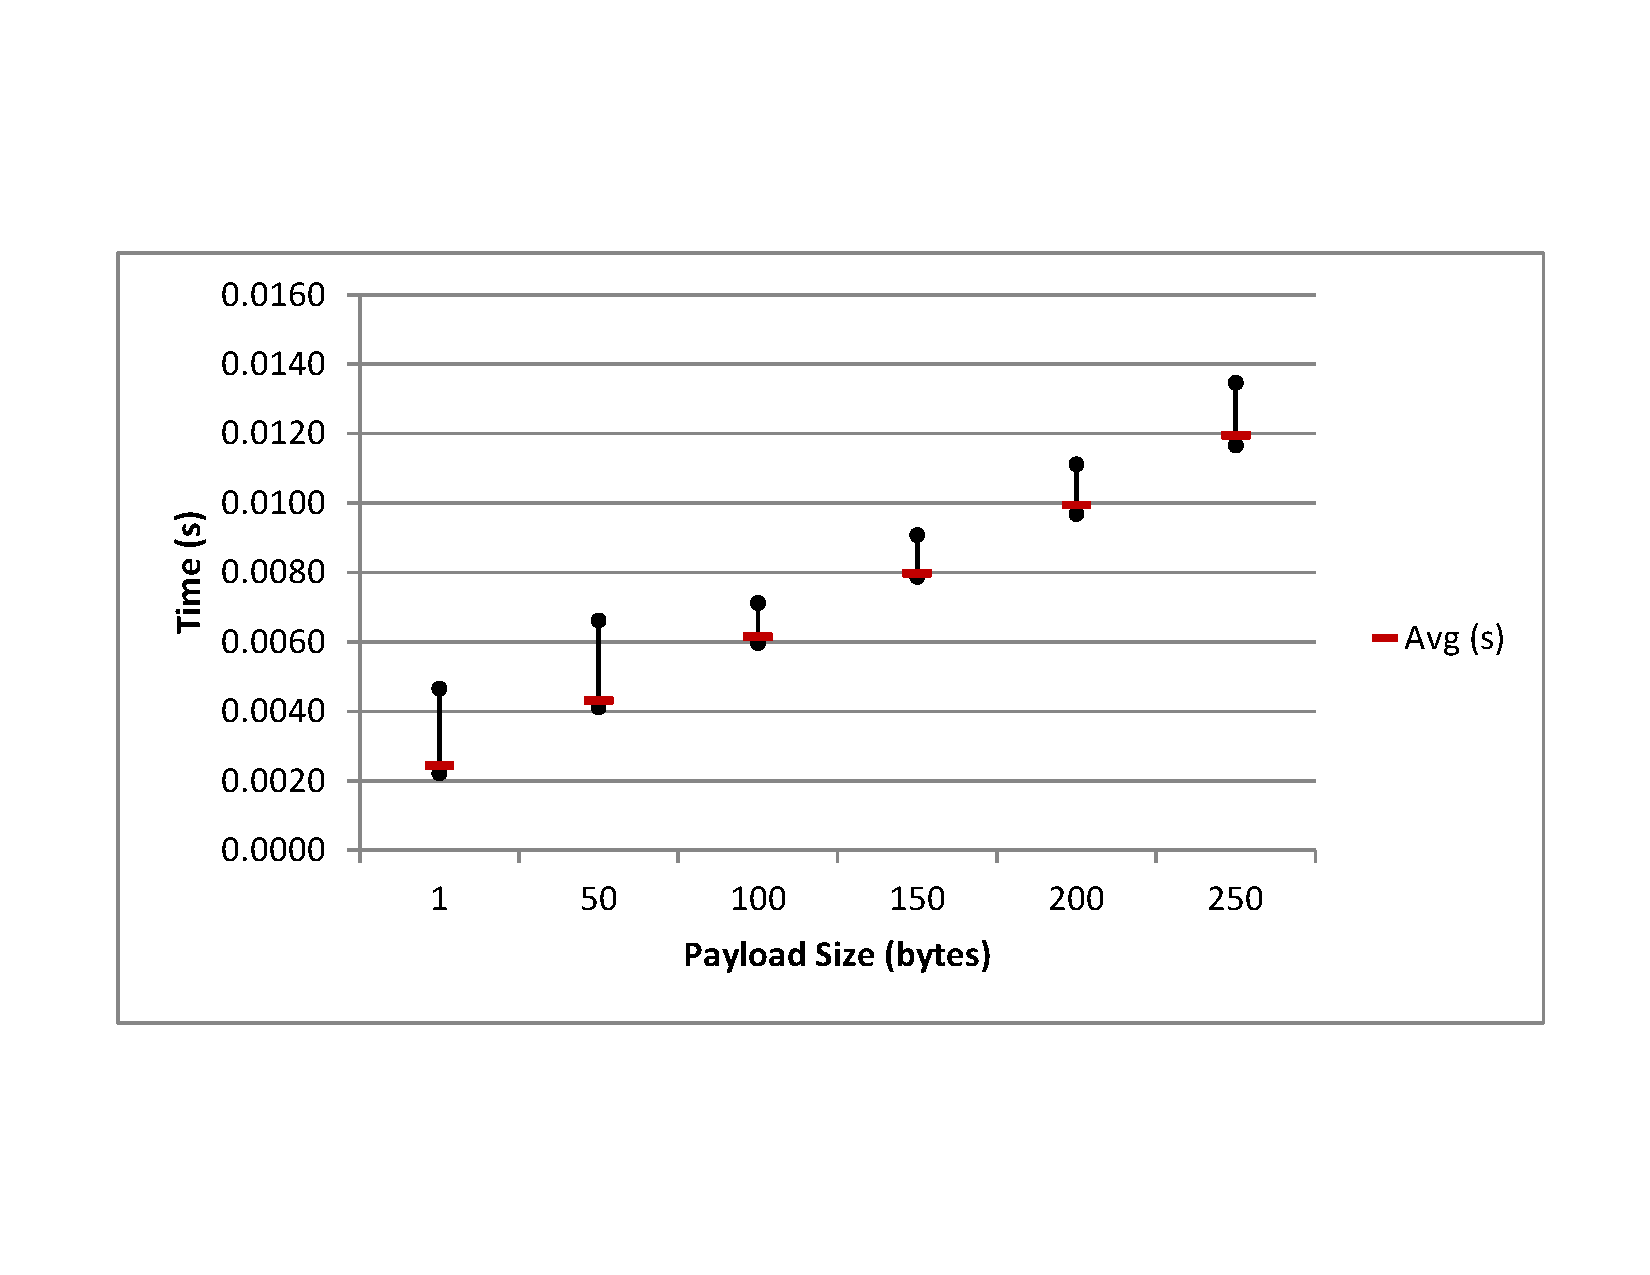
\includegraphics[width=6in]{Protocol/Figures/protocol-time_vs_size.pdf}
		\caption{Transfer time versus payload size}
		\label{fig:protocol:time_vs_size}
	\end{centering}
\end{figure}

\begin{figure}[ptb]
	\begin{centering}
		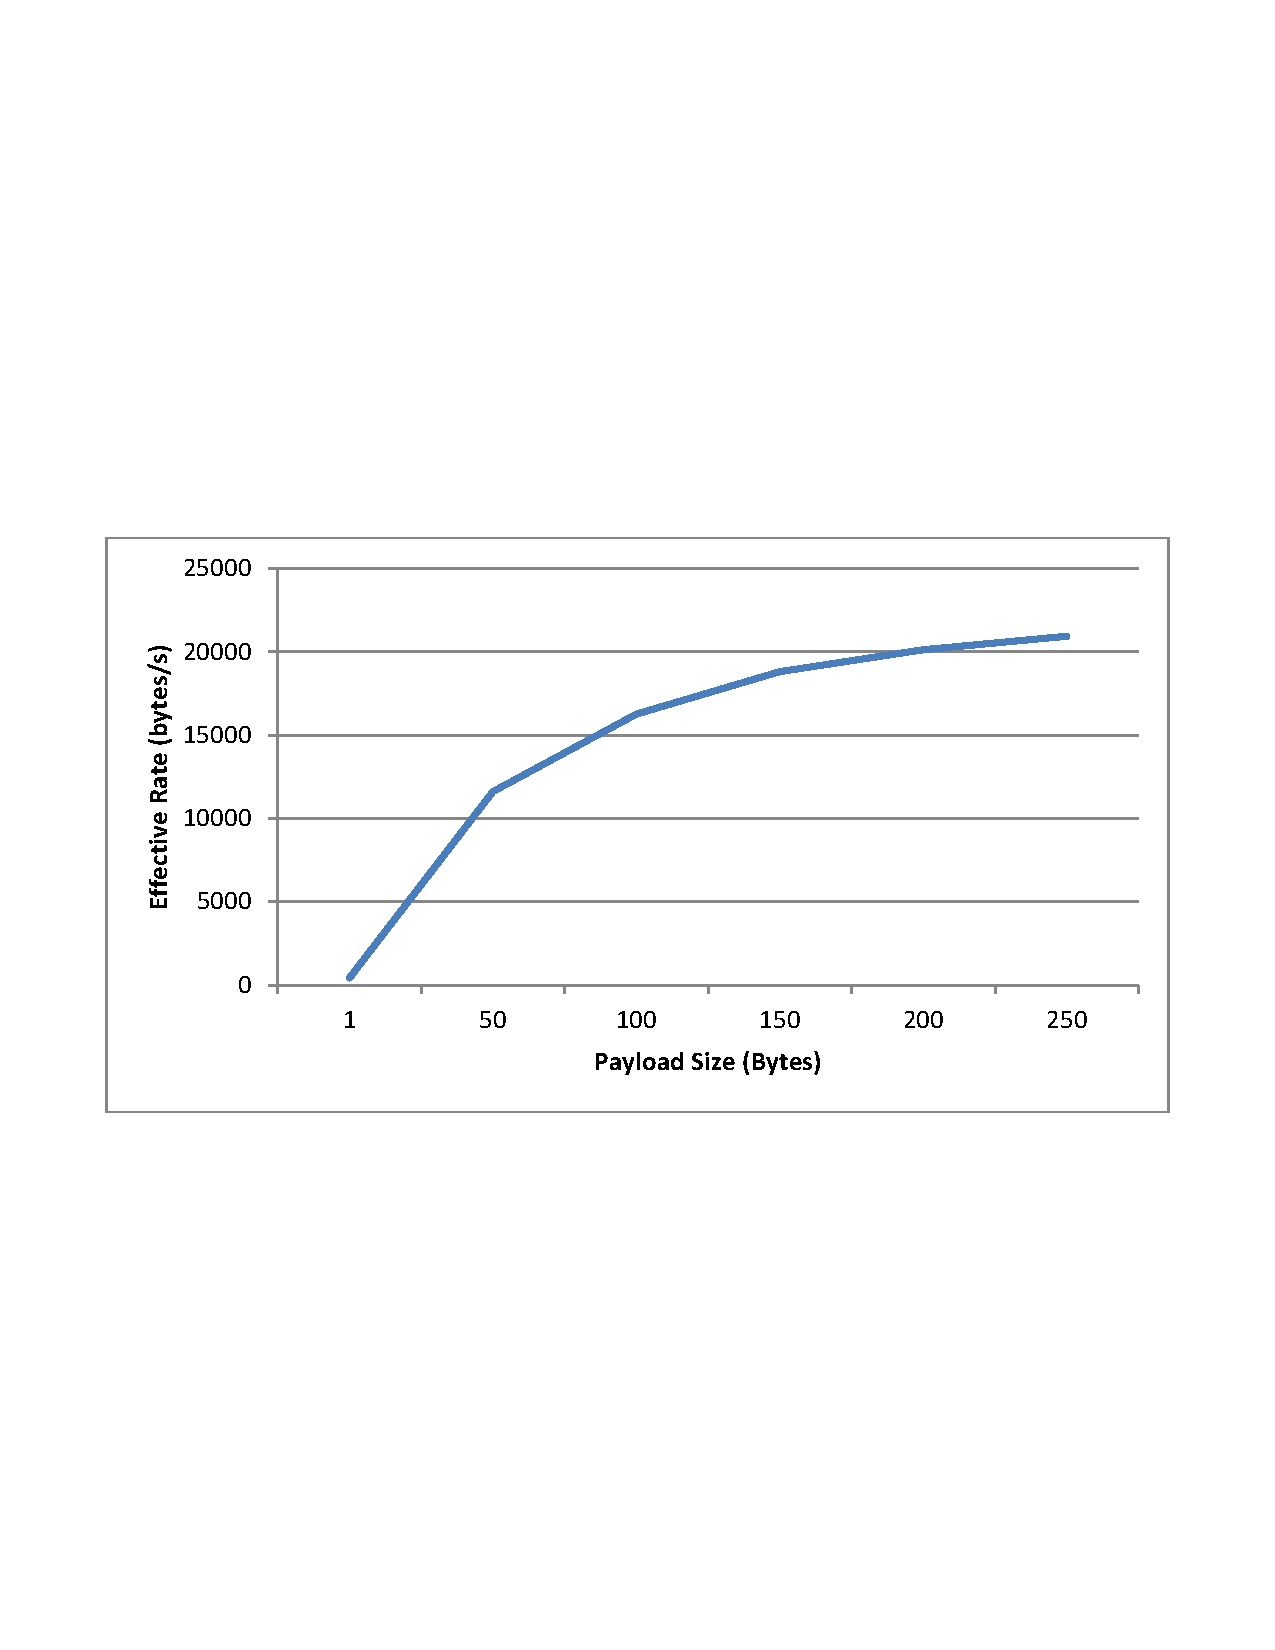
\includegraphics[width=6in]{Protocol/Figures/protocol-rate_vs_size.pdf}
		\caption{Effective transfer rate versus payload size}
		\label{fig:protocol:rate_vs_size}
	\end{centering}
\end{figure}

\begin{table}
	\begin{center}
		\setlength{\extrarowheight}{1.5pt}
		\caption{Transfer time versus payload size}
		\vspace{0.1cm}
		\begin{tabular} {|c|c|c|c|c|}
			\hline
			\textbf{Num Interm. Nodes} & \textbf{Min (s)} & \textbf{Max (s)} & \textbf{Avg (s)} & \textbf{Rate (bytes/sec)} \\
			\hline
			\hline
			0 & 0.0059 & 0.0078 & 0.0062 & 16208 \\
			\hline
			1 & 0.0082 & 0.0107 & 0.0084 & 11877 \\
			\hline
			2 & 0.0098 & 0.0110 & 0.0101 & 9940 \\
			\hline
			3 & 0.0115 & 0.0135 & 0.0119 & 8394 \\
			\hline
			4 & 0.0129 & 0.0144 & 0.0133 & 7492 \\
			\hline
			5 & 0.0146 & 0.0171 & 0.0151 & 6624 \\
			\hline
			6 & 0.0162 & 0.0189 & 0.0169 & 5910 \\
			\hline
		\end{tabular}
		\label{tab:protocol:time_vs_size}
	\end{center}
\end{table}

The second performance test is to measure the effect of distance on transfer times and effective bandwidth. This test had the root transmit a 100 byte data payload to each of the nodes, and the transfer time was recorded using the previously mentioned method. Each distance was measured 2000 times. The results are shown in Figure \ref{fig:protocol:time_vs_distance} and Table \ref{tab:protocol:time_vs_distance}. As expected, the time increases linearly as the distance is increased. The effective bandwidth versus distance is shown in Figure \ref{fig:protocol:rate_vs_distance}, and decreases as expected.

\begin{figure}[ptb]
	\begin{centering}
		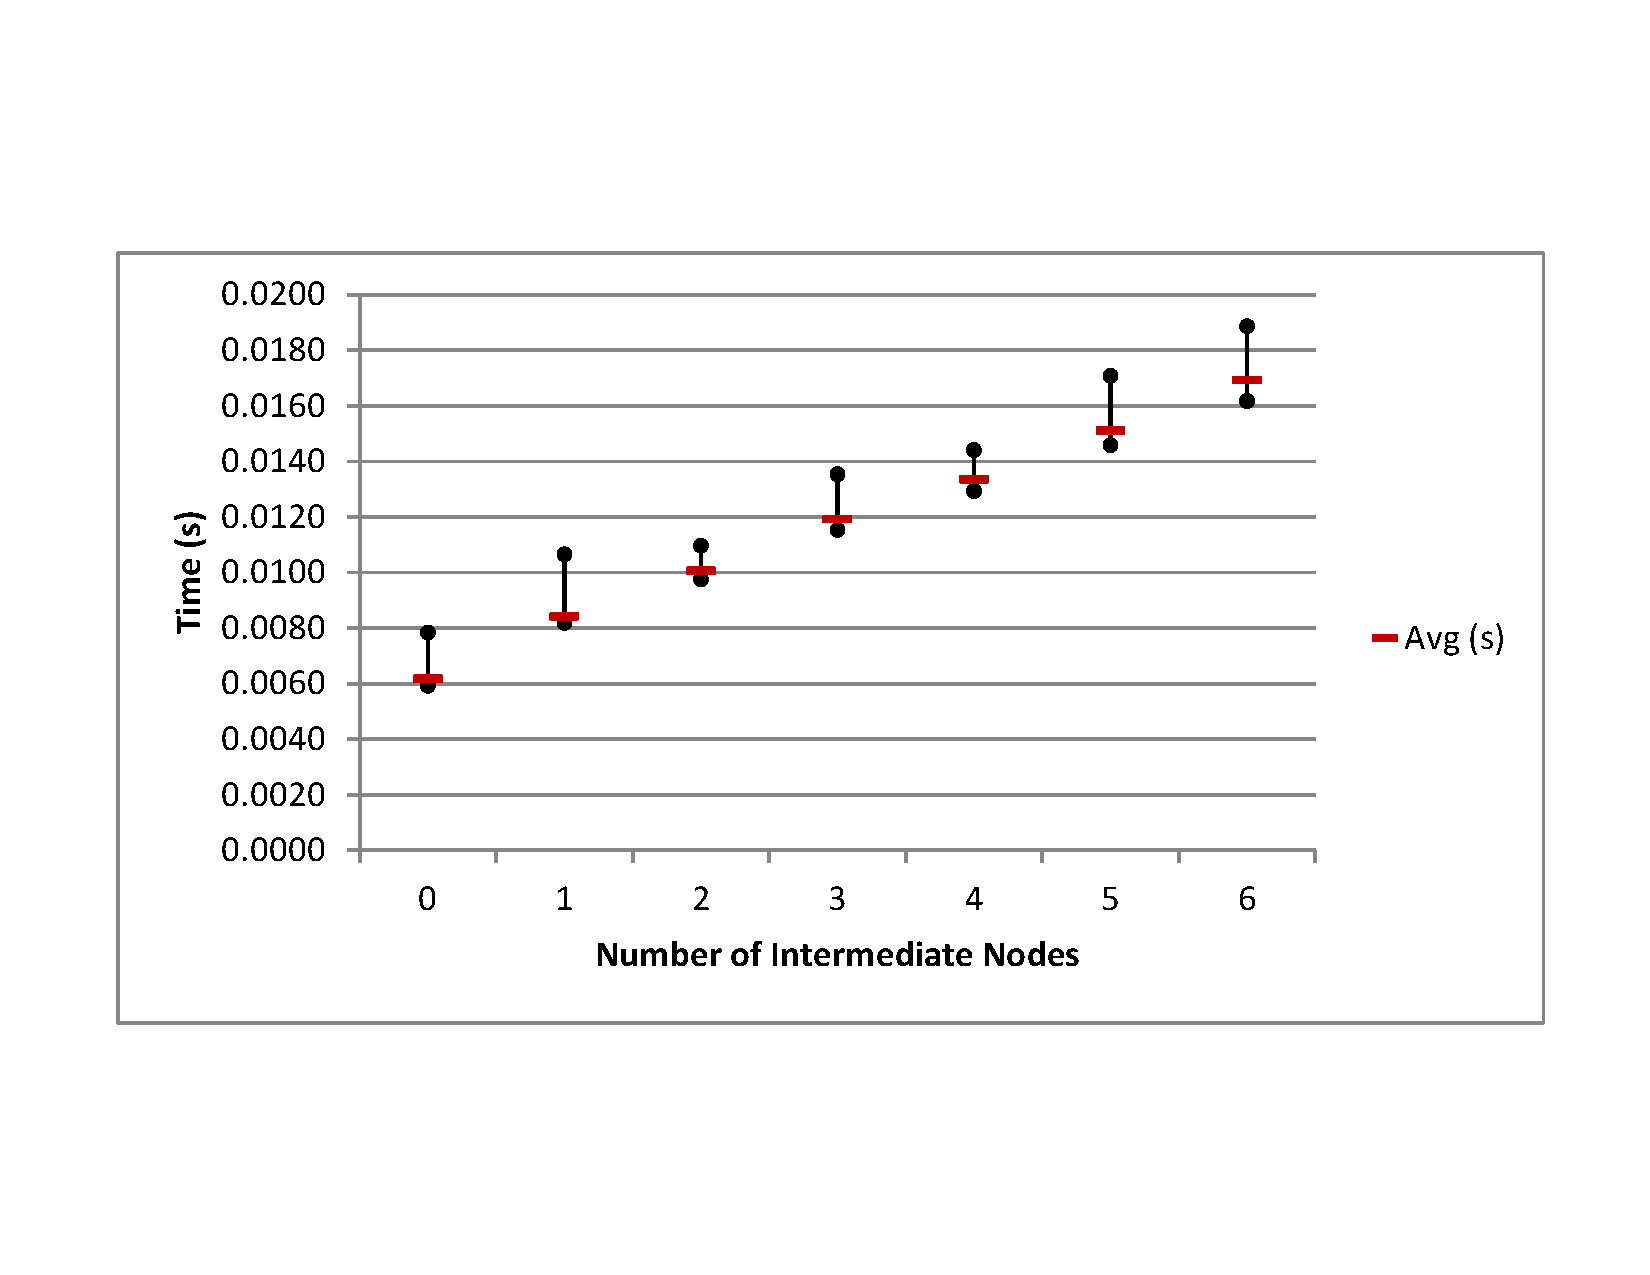
\includegraphics[width=6in]{Protocol/Figures/protocol-time_vs_distance.pdf}
		\caption{Transfer time versus transmission distance}
		\label{fig:protocol:time_vs_distance}
	\end{centering}
\end{figure}

\begin{figure}[ptb]
	\begin{centering}
		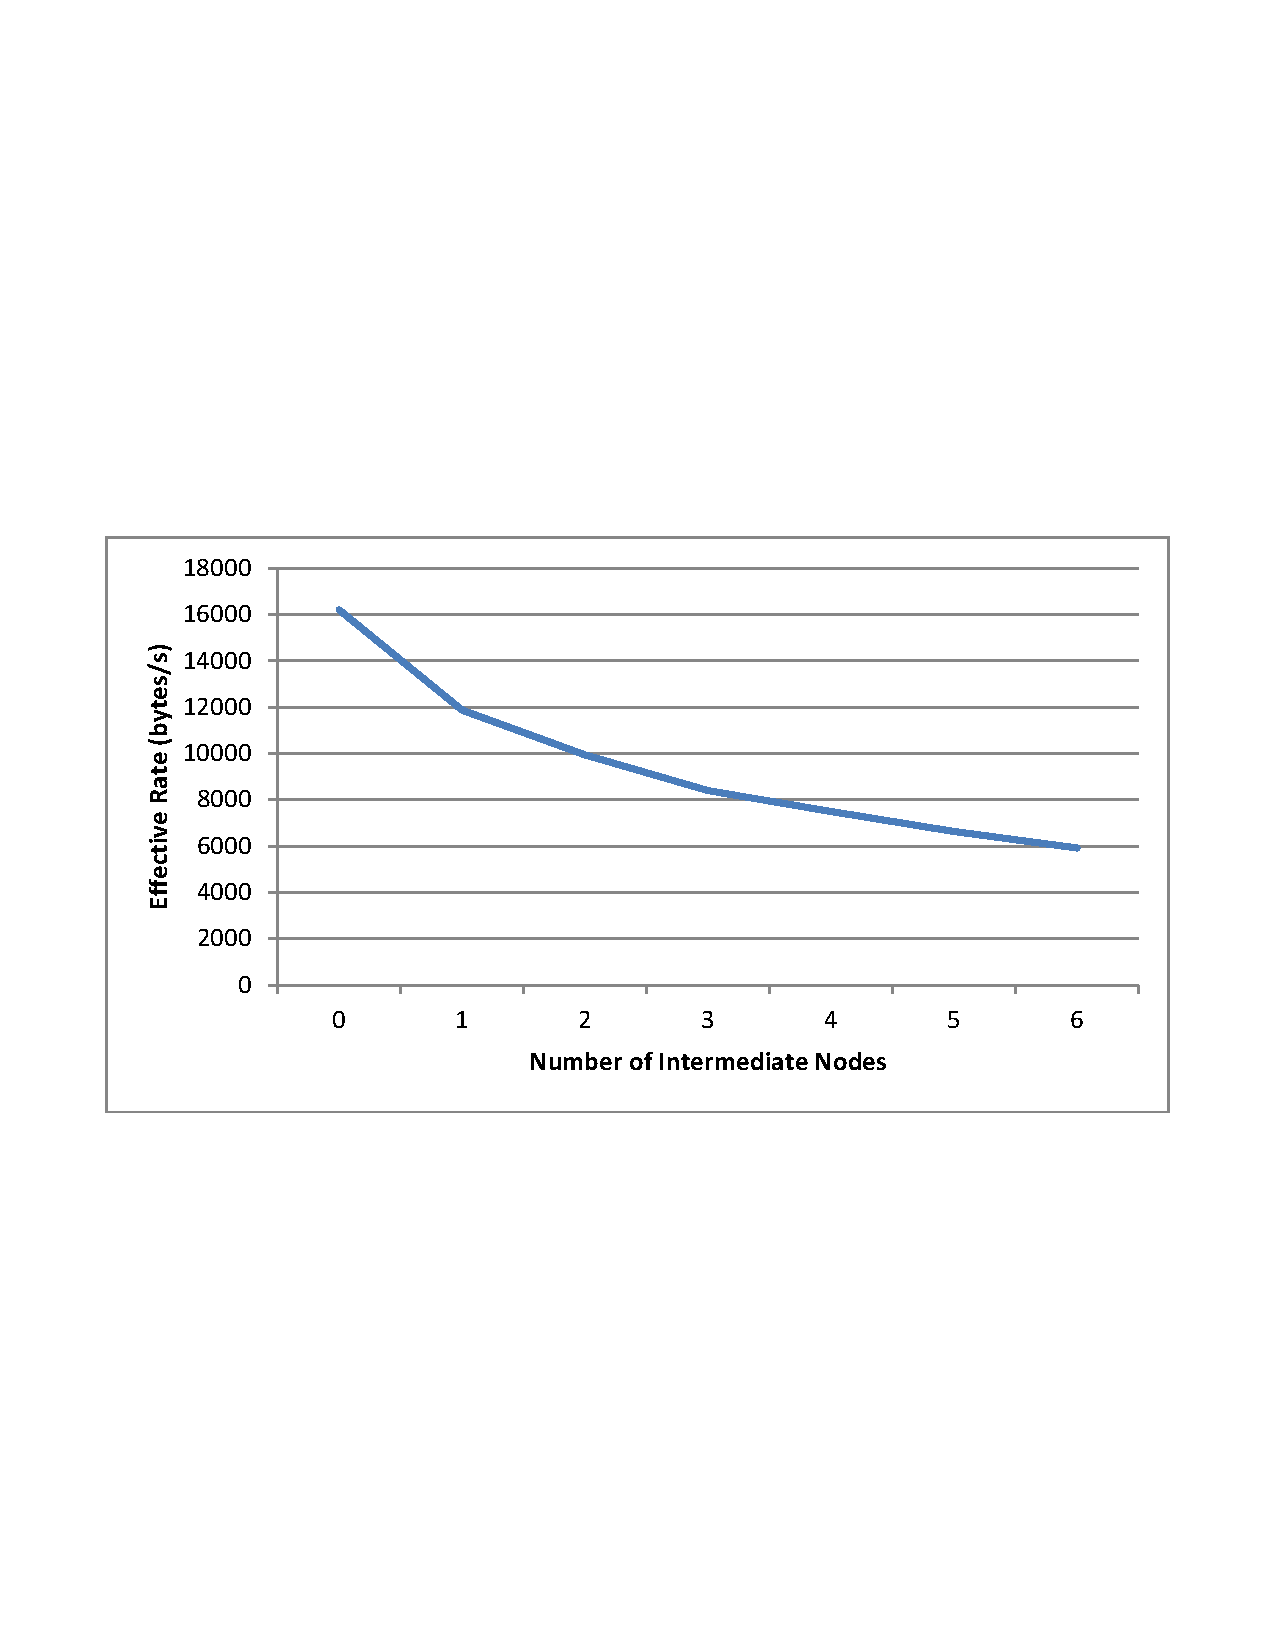
\includegraphics[width=6in]{Protocol/Figures/protocol-rate_vs_distance.pdf}
		\caption{Effective transmission rate versus transmission distance}
		\label{fig:protocol:rate_vs_distance}
	\end{centering}
\end{figure}

\begin{table}
	\begin{center}
		\setlength{\extrarowheight}{1.5pt}
		\caption{Transfer time versus transmission distance}
		\vspace{0.1cm}
		\begin{tabular}{|c|c|c|c|c|}
			\hline
			\textbf{Intm. Nodes} & \textbf{Min (s)} & \textbf{Max (s)} & \textbf{Avg (s)} & \textbf{Rate (bytes/sec)} \\
			\hline
			\hline
			0 & 0.0059 & 0.0078 & 0.0062 & 16208 \\
			\hline
			1 & 0.0082 & 0.0107 & 0.0084 & 11877 \\
			\hline
			2 & 0.0098 & 0.0110 & 0.0101 & 9940 \\
			\hline
			3 & 0.0115 & 0.0135 & 0.0119 & 8394 \\
			\hline
			4 & 0.0129 & 0.0144 & 0.0133 & 7492 \\
			\hline
			5 & 0.0146 & 0.0171 & 0.0151 & 6624 \\
			\hline
			6 & 0.0162 & 0.0189 & 0.0169 & 5910 \\
			\hline
		\end{tabular}
		\label{tab:protocol:time_vs_distance}
	\end{center}
\end{table}

The final performance test is to measure latency versus distance. Latency can be defined a number of ways; here it is defined as the length of time that passes between calling a transmit function and the instant that the first control ACK is finished processing in the protocol stack. For these tests, a data transfer was used to perform the test because the basic test was already set up from the previous tests. The timer was started when the transmit data packet function was called and was stopped when the transfer request received sequence step had finished processing. The results are shown in Figure \ref{fig:protocol:latency_vs_distance} and Table \ref{tab:protocol:latency_vs_distance}. As expected, latency increases linearly with distance.

\begin{figure}[ptb]
	\begin{centering}
		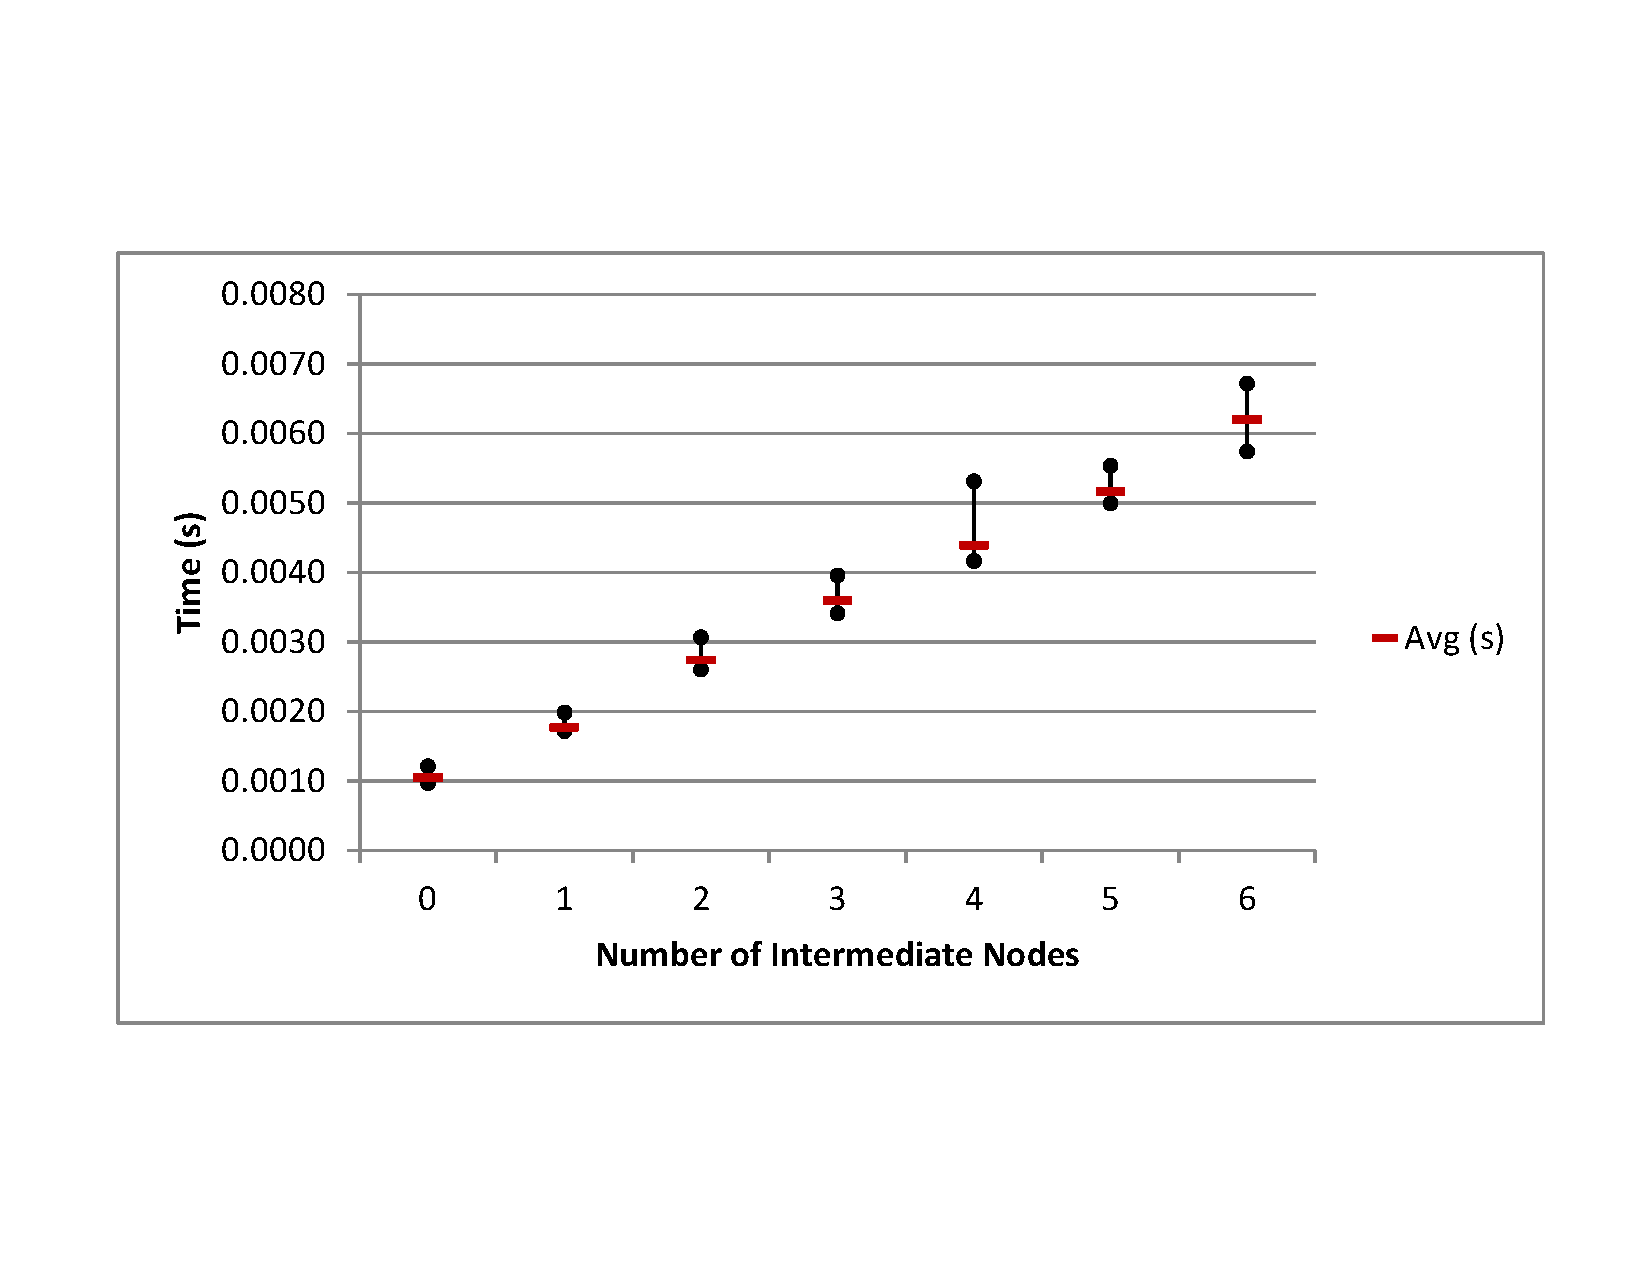
\includegraphics[width=6in]{Protocol/Figures/protocol-latency_vs_distance.pdf}
		\caption{Latency versus transmission distance}
		\label{fig:protocol:latency_vs_distance}
	\end{centering}
\end{figure}

\begin{table}
	\begin{center}
		\setlength{\extrarowheight}{1.5pt}
		\caption{Latency versus transmission distance}
		\vspace{0.1cm}
		\begin{tabular} {|c|c|c|c|}
			\hline
			\textbf{Intm. Nodes} & \textbf{Min (s)} & \textbf{Max (s)} & \textbf{Avg (s)} \\
			\hline
			\hline
			0 & 0.0010 & 0.0012 & 0.0010 \\
			\hline
			1 & 0.0017 & 0.0020 & 0.0018 \\
			\hline
			2 & 0.0026 & 0.0031 & 0.0027 \\
			\hline
			3 & 0.0034 & 0.0040 & 0.0036 \\
			\hline
			4 & 0.0042 & 0.0053 & 0.0044 \\
			\hline
			5 & 0.0050 & 0.0055 & 0.0052 \\
			\hline
			6 & 0.0057 & 0.0067 & 0.0062 \\
			\hline
		\end{tabular}
		\label{tab:protocol:latency_vs_distance}
	\end{center}
\end{table}

\section{Future Work}\label{sec:protocol:future_work}

One aspect that is highlighted by the results is that general processing on the F2808 is very slow, which is expected. Branching and other non-data intensive instructions on DSPs tend to be slow because DSPs are special-purpose devices geared towards streaming mathematical computation. This explains the relatively poor performance of the protocol stack on the F2808, because the protocol stack consists almost entirely of branching code. There are a variety of potential applications where using multiple F2808s in parallel would be advantageous. The F2808 was primarily designed for high-performance motor control. A potential system would be one that contains multiple motors with multiple inputs being run through multiple PID loops that must also come to a consensus, where a network of F2808s would shine. There are also potential applications where using a more general purpose processor, such as an ARM or PowerPC processor, would be more appropriate. These general purpose processors would improve performance of the protocol, but other mechanisms can also improve protocol performance in scenarios where a DSP is a better fit, such as attempting to minimize overhead. One method of minimizing overhead is to combine smaller data payloads into a single larger payload that is then divided up at the source after reception. Switching to wormhole routing would also reduce overhead but could also cause resource allocation problems, because many resources are taken up when a transfer gets blocked. In addition communication faults become possible, so mechanisms would have to be implemented to prevent them. As of the time of this writing, multicast and broadcast transmissions have not been implemented, and would increase efficiency of for certain types of communications.

Another area in need of improvement is path storage in the packet header. Systems are currently limited to 16 nodes with a maximum path length of 8. This limitation can be overcome by getting the path to use full 8-bit addresses. A larger bit size increases the space needed to store the path, so another mechanism that can be used is to store partial paths, i.e. a packet is transmitted along the path stored in the packet until it reaches the end of the path, where the next path segment is generated. This mechanism would allow unlimited path lengths. The packet header could also be lengthened to allow longer path lengths, but this would also require changes to the data link and physical layers to accommodate larger flit sizes.

\section{Conclusions}\label{sec:protocol:conclusions}

In this chapter, a custom protocol has been described that serves as the network layer in the prototype toolkit. A fixed packet header has been defined that uses commands and sequence steps to identify the purpose of the packet. Error detection has been implemented in the form of CRC checks for both headers and data payloads. Guaranteed delivery is left for higher level layers. An addressing scheme has been devised that provides completely dynamic addressing and is coordinated by a ``root'' node. The root node also coordinates routing table generation and distribution. Data transfers use pipelined circuit switching to maximize robustness and minimize in-flight resource usage. Nodes continuously check to ensure that their neighbors are still communicating, and if not, they notify the root node so that the faulty node can be removed from the routing table. This mechanism has shown to be reliable and has performance that is adequate, if not exactly stellar, for coarse grained parallel computing.